\documentclass[12pt]{memoireuqam1.3}

\usepackage{graphicx}% Pour les figures
\usepackage[latin1]{inputenc} % Pour utiliser les caractères accentués
\usepackage[francais]{babel}
\usepackage{textcomp}
\usepackage[toc,page]{appendix} 
\usepackage{caption}
\usepackage{url}
\usepackage[round]{natbib}
\usepackage{multirow}
\usepackage{longtable}
\usepackage{amssymb}
\usepackage[algochapter,linesnumbered]{algorithm2e}
\usepackage[T1]{fontenc}
\usepackage{url}
\usepackage{pdfpages}
%\input macro  % Pour les définitions personnelles

\newcommand{\red}[1]{#1} %MAJOR CHANGES
\newcommand{\blue}[1]{#1} %MINOR CHANGES
\newcommand{\green}[1]{#1} % TO DO
\newcommand{\comment}[1]{}  

\newtheorem{hypothesis}{Hypoth\`ese}[chapter]
\newtheorem{change}{Changement}[chapter]

\SetAlgorithmName{Algorithme}{algorithme}{Liste d'Algorithmes}

\let\oldemptyset\emptyset
\let\emptyset\varnothing

\begin{document}

%%%%%%%%%%%%%%%%%%%%
% Pour la page titre
%%%%%%%%%%%%%%%%%%%%
\title{Am\'elioration de la D\'etection d'Anti-Patrons dans les Syst\`emes \`a Base de Services par la Fouille de Traces d'Ex\'ecution}
\author{Mathieu Nayrolles}
% Année et mois courant sauf si spécifié autrement pas \degreemonth et \degreeyear
\degreemonth{Mars}
\degreeyear{2014}
\uqammemoire %% ou \uqamthese ou \uqamrapport
\matiere{informatique}


\thispagestyle{empty}        % La page titre n'est pas numérotée
\maketitle

%%%%%%%%%%%%%%%%%%%%
% Page préliminaires
%%%%%%%%%%%%%%%%%%%%
\renewcommand \bibname{R\'EF\'ERENCES}% FACULTATIF
%si vous voulez qu'apparaisse le titre RÉFÉRENCES plutôt que BIBLIOGRAPHIE

\renewcommand \listfigurename{LISTE DES FIGURES}
\renewcommand \appendixname{APPENDICE}
\renewcommand \figurename{Figure}
\renewcommand \tablename{Tableau}

\pagenumbering{roman} % numérotation des pages en chiffres romains
\addtocounter{page}{1} % Pour que les remerciements commencent à la page ii
\chapter*{Remerciements}

Au cours de ces mois au Canada, de nombreuses personnes m'ont aid� et soutenu afin que je puisse m'int�grer au mieux dans ce nouveau pays ainsi que dans cette nouvelle universit�.
Ce sont ces personnes que je souhaite remercier tout particuli�rement.

Pr.Naouel Moha, ma directrice de recherche pour m'avoir initi� � la qualit� logicielle et aux applications � base de services.
Je la remercie �galement pour sa disponibilit� constante et pour m'avoir fait d�couvrir le monde de la recherche.
Pr.Petko Valtchev, mon codirecteur de recherche pour avoir accept� de me co-encadrer dans mes recherches et m'avoir initi� au monde de la fouille de donn�es.

Pr. Privat, Pr. Beaudry et Pr. Tremblay pour les connaissances acquises dans leurs cours respectifs de principes avanc�s de langages � objets, planification eb intelligence artificielle et parall�lisme hautes performances.
Je remercie aussi Messieurs Berger et Levesque d'avoir fait appel � moi pour les assister dans leurs cours respectifs de Programmation Agile et Mod�lisation avanc�e.

Alexandre Sbriglio, pilote du cycle sup�rieur eXia.Cesi d'Aix-En-Provence, pour m'avoir suivi de pr�s malgr� la distance et pour m'avoir d�charg� de nombreux soucis li�s � ma vie au Canada ou aux interactions entre l'UQAM et l'eXia.Cesi.

Pr. Yann-Ga�l Gu�h�neuc de l'\'Ecole Polytechnique de Montr�al pour m'avoir donn� acc�s aux diff�rentes recherches men�es dans son laboratoire, m'avoir invit� � certains s�minaires, et pour nos discussions sur la g�n�ricit� en Java.
Pr. Abdelwahab Hamou-Lhadj de l'Universit� de Concordia, pour avoir particip� � la maturation de nos id�es et approches bas�es sur les traces d'ex�cutions.

Je souhaite aussi remercier Phillipe Merle et Lionel Seinturier pour leurs validations de notre approche sur le syst�me \textit{FraSCAti} et Francis Palma pour la sa validation du syst�me \textit{Home-Automation}.

Les stagiaires du LATECE, �tudiants � la ma�trise et au doctorat, qui ont contribu� � cr�er une atmosph�re de travail agr�able et qui ont toujours �t� disponibles en cas de besoin.
Guillaume, Benjamin, Nicolas, Choukri, Gino, Anis, Anthony, Francis et tous ceux que je ne peux pas citer.
Les personnes qui ont contribu�s � rendre ma vie � Montr�al plus qu'agr�able : Samuel, Clarisse, David, Tiphaine, S�bastien, Benjamin et tant d'autres.

Caroline Lafarie-Gremillet et Marie De Abreu pour les relectures profondes et compl�tes de ce m�moire.

Finalement, Lakm� Gremillet pour m'avoir soutenu au travers de cette ma�trise et ce, quel que soit les doutes et les difficult�s.
\tableofcontents % Pour générer la table des matières
\listoftables % Pour générer la liste des tableaux
\listoffigures % Pour générer la liste des figures
\begin{abstract}
Les syst�mes � base de services (SBSs), � l'instar des autres syst�mes complexes, �voluent pour s'adapter � des nouvelles demandes utilisateurs et � de nouveaux contextes d'ex�cution.
Cette �volution continue peut facilement d�t�riorer la qualit� de service (QoS) et de conception des SBSs et introduire des d�fauts de conception, connus sous le nom d'anti-patrons SOA (\textit{Service Oriented Architecture}).
Les anti-patrons de conception sont des solutions r�currentes et reconnues sous-optimums � des probl�mes connus.
Les anti-patrons sont donc l'inverse des patrons de conception qui sont de bonnes solutions � des probl�mes connus.
Les anti-patrons SOA conduisent � une maintenabilit� et une r�utilisabilit� r�duites des SBSs.
Il est donc important de les d�tecter puis de les supprimer.
Cependant, les techniques pour leur d�tection en sont � leurs balbutiements, et il n'y a actuellement qu'un seul outil, nomm� SODA (\textit{Service Oriented Detection for Antipatterns}), permettant leur d�tecion automatique.
SODA est bas� sur un ensemble de m�triques majoritairement statiques et sur quelques m�triques dynamiques qui sont calcul�es lors de l'ex�cution du syst�me cible gr�ce � des techniques de programmation orient�e aspect.
Dans ce m�moire, nous proposons une nouvelle approche nomm�e SOMAD (\textit{Service Oriented Mining for Antipatterns Detection}) qui est une �volution de SODA.
Le but de notre nouvelle approche est d'am�liorer la d�tection automatique des anti-patrons SOA en fouillant les traces d'ex�cution que produisent les SBSs.
En effet, les traces d'ex�cution repr�sentent plusieurs avantages qui permettront d'am�liorer la d�tection car elles permettent de capturer pleinement la nature hautement dynamique des SBSs tout en n�cessitant un niveau de contr�le relativement faible sur les syst�mes cibles.
SOMAD mine des r�gles d'association pertinentes dans les traces d'ex�cution des SBSs, puis les filtre via une suite de m�triques d�di�es.
Nous discutons d'abord les mod�les de r�gles d'association sous-jacents et les intuitions soutenant les m�triques d�di�es aux SBSs.
Les r�gles d'association permettent de d�couvrir des relations entre diff�rents objets dans un grand ensemble de donn�es.
Nous pr�sentons aussi deux exp�rimentations visant la validation formelle de notre approche.
Une comparaison entre SOMAD et SODA est effectu�e et r�v�le l'efficacit� de SOMAD face � SODA: sa pr�cision est meilleure d'une marge allant de 8.3\% � 20\% tout en gardant le rappel � 100\%.
Finalement, SOMAD est, au minimum, 2.5 fois plus rapide que SODA sur les m�mes sujets d'exp�rimentation.
\end{abstract}

% Utilisez l'environnement  abstract pour rédiger votre résumé


%%%%%%%%%%%%%%%%%%%%
% Document principal
%%%%%%%%%%%%%%%%%%%%

\begin{introduction}

\section*{Contexte de l'\'etude: Les applications \`a base de services et les anti-patrons}

Les syst\`emes \`a base de service (SBSs) sont compos\'es de services d\'ej\`a pr\^ets et accessibles par Internet \citep{Erl2008}.
Les services sont des unit\'es logicielles autonomes, interop\'erables, et r\'eutilisables qui peuvent \^etre impl\'ement\'ees en utilisant un large choix de technologies tels que les services web, REST (\textit{REpresentational State Transfert}), ou SCA (\textit{Service Component Architecture}, une surcouche au SOA).
La plupart des plateformes web connues du grand public sont de parfaits exemples de SBSs comme Amazon, PayPal et eBay.
De tels syt\`emes sont complexes --- ils g\'en\`erent des fl\^ots massifs de communication entre les services --- et hautement dynamiques: des services apparaissent, disparaissent ou sont modifi\'es.
L'\'evolution constante des SOAs (\textit{Service Oriented Architecture Systems}) peut facilement d\'et\'eriorer la qualit\'e de leurs architectures par l'introduction de d\'efauts architecturaux connus sous le nom d'anti-patrons SOA \citep{Moha}.
Un anti-patron de conception est une solution connue et non-optimale \`a un probl\`eme connu.
Les anti-patrons sont oppos\'es aux patrons de conception qui sont eux des bonnes pratiques en r\'eponse \`a des probl\`emes connus.
Les anti-patrons peuvent donc \^etre qualifi\'es de mauvaises pratiques de conception.

Par exemple, le \textit{Tiny Service} est un anti-patron  largement r\'epandu dans les syst\`emes \`a base de services.
Ce service a une tr\`es petite taille avec tr\`es peu de m\'ethodes qui impl\'ementent seulement une partie d'une abstraction \citep{Dudney2003}.
Les \textit{Tiny Services} sont g\'en\'eralement accompagn\'es de plusieurs autres services fortement coupl\'es, ce qui induit une complexit\'e dans le d\'eveloppement et r\'eduit la r\'eutilisabilit\'e.
De plus, il a \'et\'e prouv\'e que les \textit{Tiny Services} sont une des principales raisons d'\'echecs (\textit{failure}) des syst\`emes \`a base de services \citep{Kral2009}.


\section*{Probl\`eme \'etudi\'e : La d\'etection des anti-patrons}

\'Etant donn\'e l'impact n\'efaste des anti-patrons sur la r\'eutilisabilit\'e et la maintenabilit\'e des SBS, il existe un besoin clair et urgent de techniques et d'outils visant leur d\'etection.
Cependant, la nature hautement dynamique et distribu\'ee des SBSs rend la d\'etection automatique des anti-patrons SOA compliqu\'ee.
C'est un v\'eritable d\'efi, surtout en comparaison avec d'autres outils visant la d\'etection d'anti-patrons dans les syst\`emes objets \citep{Marinescu2004, Fokaefs2007, Moha2010}.
En 2012, notre \'equipe, compos\'ee de Naouel Moha, Francis Palma, Benjamin Joyen-Conseil, Yann-Ga\"el Gu\'eh\'eneuc, Benoit Beaudry, Jean-Marc J\'ez\'equel et moi m\^eme, a d\'evelopp\'e une approche nomm\'ee SODA (\textit{Service Oriented Detection for Anti-patterns}) \citep{Nayrolles, Moha} qui vise la d\'etection des anti-patrons SOA.
Cette approche repose sur un langage sp\'ecifique au domaine (\textit{Domain Specific Language}, DSL) pour sp\'ecifier les anti-patrons SOA et est bas\'ee sur des m\'etriques (majoritairement statiques) d'un c\^ot\'e, et sur une m\'ethode de g\'en\'eration automatique d'algorithmes de d\'etection, de l'autre.


Bien qu'\'etant efficace et pr\'ecise, SODA souffre de s\'erieuses limitations.
En effet, SODA ex\'ecute deux phases d'analyse, une premi\`ere statique, suivie d'une seconde, dynamique.
La premi\`ere analyse statique requiert un acc\`es aux interfaces des services.
En cons\'equence, SODA ne peut pas analyser dont les sources ne sont pas disponible.
La seconde phase, \red{\`a moindre port\'ee}, d'analyse dynamique requiert l'\'ex\'ecution concr\`ete du syst\`eme et de ce fait, la cr\'eation de sc\'enarios ex\'ecutables.
De plus, SODA a \'et\'e cr\'e\'e sp\'ecifiquement pour les syst\`emes de type SCA et sa pr\'ecision tend \`a faiblir lorsque la taille des syst\`emes augmente.
\'Etant donn\'e les limitations de SODA, il y a un \red{espace pour l'am\'elioration de} nos approches et outils pour la d\'etection d'anti-patrons SOA.
Ces am\'eliorations doivent apporter une d\'etection pr\'ecise, efficace et applicable \`a toutes les technologies SOA (REST, SCA, service web, ...) et ce quelque soit la taille du syst\`eme.
Dans ce m\'emoire, nous proposons une approche nomm\'ee SOMAD (\textit{Service Oriented Mining for AntiPatterns Detection}).
Cette approche ne requiert pas de sc\'enarios, \`a l'inverse de SODA, et repose uniquement sur les traces d'ex\'ecution qui peuvent \^etre disponibles dans toutes les technologies SOA.
SOMAD est capable d'\'eliminer les donn\'ees non pertinentes en utilisant une technique de fouille de donn\'ees: la fouille de r\`egles d'association s\'equentielle.
La fouille de r\`egles d'association \citep{Agrawal1994} et a fortiori la fouille de r\`egles d'association s\'equentielles -- en particulier l'algorithme \textit{RuleGrowth} \citep{Fournier-viger2011} -- sont des m\'ethodes servant \`a d\'ecouvrir des relations int\'eressantes dans de larges bases de donn\'ees.
SOMAD \red{applique} ses m\'ethodes sur les traces d'ex\'ecution pour d\'ecouvrir des anti-patrons SOA \red{sous forme de configurations particuli\`eres dans la composition des r\`egles d'association.} Pour ce faire, nous utilisons une variante de la fouille de r\`egles d'association bas\'ee sur les s\'equences ou \'episodes.
Dans notre cas, les s\'equences repr\'esentent \red{des suites d'appels} de services et de m\'ethodes.
Ensuite, nous filtrons ces r\`egles d'association en utilisant une suite de m\'etriques \red{d\'edi\'ees afin d'}extraire la connaissance pertinente des r\`egles d'association.

\section*{Contributions}

Les principales contributions li\'ees \`a ce m\'emoire sont les suivantes:

\begin{enumerate}
\item Une nouvelle approche nomm\'ee SOMAD pour la d\'etection des anti-patrons SOA.
Cette approche est bas\'ee sur des r\`egles d'association fouill\'ees sur des traces d'ex\'ecution qui peuvent provenir de toutes les technologies SOA.
\item une validation empirique de notre approche qui d\'emontre l'am\'elioration apport\'ee par SOMAD en terme de pr\'ecision (8.3\% \`a 20\%) et de vitesse (2.5 fois plus rapide).
\item Une \'evolution de l'algorithme \textit{RuleGrowth} visant la fouille de r\`egles d'association s\'equentielles dans des s\'equences d'appels des SBSs.
De ce fait, nous am\'eliorons la d\'etection d'anti-patrons SOA.
\end{enumerate}

Les contributions 1 et 2 ont \'et\'e pr\'esent\'ees \`a la $20^{ieme}$ \'edition de la conf\'erence internationale de travail sur la r\'etro-ing\'enierie (WCRE 2013, \textit{Working Conference on Reverse Engineering}) \citep{Nayrolles2013a}.

\section*{Structure du document}

Ce m\'emoire est organis\'e de la mani\`ere suivante. Les deux premiers chapitres pr\'esentent respectivement l'\'etat de l'art sur la d\'etection de patrons de conceptions et l'extraction de connaissances depuis les traces d'ex\'ecution.
Le troisi\'eme chapitre, quant \`a lui, pr\'esente l'approche SOMAD.
Le quatri\'eme pr\'esente l'impl\'ementation de \textsc{Somad} tandis que le cinqui\`eme et dernier chapitre pr\'esente nos exp\'erimentations. Enfin, nous proposons quelques remarques de fin dans la conclusion.

\end{introduction}
% Utilisez l'environnement  introduction pour rédiger votre introduction
\chapter{\'Etat de l'art sur la d\'etection de patrons de conception}



%L'approche SOMAD repose sur deux champs de recherches distincts: la d\'etection d'anti-patrons et l'extraction de connaissances depuis les traces d'association. La section \ref{rel1} pr\'esente les travaux de l'\'etat de l'art concernant la d\'etection de patrons et d'anti-patrons qu'ils soient orient\'es objets ou services. La section \ref{rel2}, quant \`a elle, pr\'esente les travaux de l'\'etat de l'art en acquisition de connaissances depuis les traces d'ex\'ecution. Finalement, la section \ref{soda} pr\'esente SODA, la seule approche existante pour la d\'etection d'anti-patrons SOA que nous avons propos\'ee dans \citep{Moha, Nayrolles, palma} et sur laquelle SOMAD est bas\'e.

%

%\section{D\'etection de Patrons et Anti-Patrons\label{rel1}}

%

%\comment{Voir journal paper + francis proposal + "Mining Rare Association Rules in the Datasets with Widely Varying Items? Frequencies" +  Cornelissen et al to get an overview of knowledge extraction from execution traces.}


Conserver une bonne qualit\'e architecturale est essentiel pour construire des syst\`emes maintenables et \'evolutifs. Les patrons et anti-patrons ont \'et\'e reconnus comme une des meilleures fa�ons d'exprimer ces pr\'eoccupations architecturales. Cependant, au contraire des anti-patrons orient\'es objet, la d\'etection de leurs \'equivalents orient\'es services en est encore \`a ses d\'ebuts.


Dans ce chapitre d\'edi\'e \`a l'\'etat de l'art sur la d\'etection de patrons de conception, nous verrons tout d'abord la d\'etection des anti-patrons objet suivi par la d\'etection de patrons SOA. Ensuite, une troisi\`eme sous section couvrira l'\'etat de l'art de la d\'etection d'anti-patrons SOA. Finalement, nous expliquerons le fonctionnement du seul outil, nomm\'e SODA, permettant la d\'etection automatique d'anti-patrons SOA.



\section{D\'etection d'anti-patrons orient\'es objets}


%\red{En total contraste avec la d\'etection d'anti-patrons SOA, la d\'etection d'anti-patrons objet est sujette \`a des recherches intensives depuis de nombreuses ann\'ees.

Ce champs de recherche est toujours largement ouvert, m\^eme si les contributions r\'ecentes se r\'ev\`elent plus incr\'ementales que r\'eelement nouvelles.

Un nombre important d'approches et d'outils existent pour la d\'etection d'anti-patrons objet \citep{Lanza2006, Moha2010, Kessentini2010,Kessentini2011} et de nombreux livres ont aussi port\'e sur le sujet.
En effet, \citet{Brown1998} ont produit un catalogue de 40 anti-patrons tandis que Beck, dans le livre \`a succ\`es \textit{Refactoring} de \citet{Fowler1999}, a identifi\'e 22 mauvaises odeurs de code (ou \textit{code smells} en anglais) qui doivent \^etre traqu\'ees et \'elimin\'ees afin d'avoir un code de meilleure qualit\'e.
\red{Un exemple simple d'anti-patron orient\'e objet est le \textit{``blob''}, aussi connu sous le nom de \textit{``god object''} (figure \ref{blob}), correspond \`a un contr�leur de grande taille (grand nombre d'attributs et de m\'ethodes) qui d\'epend de donn\'ees stock\'ees dans des classes adjacantes.

Le blob est une tr\`es grande classe qui d\'eclare de nombreux champs et m\'ethodes avec une faible coh\'esion.
Une classe de type contr�leur monopolise la majorit\'e du traitement effectu\'e par le syst\`eme, prend la majorit\'e des d\'ecisions et dirige le traitement eff\'ectu\'e par les autres classes.
De plus, il est fortement coupl\'e aux classes de donn\'ees adjacentes.}


\begin{figure}

\begin{center}

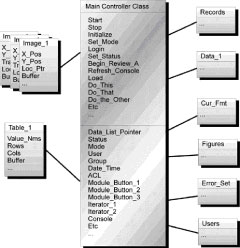
\includegraphics{media/blob.jpg}

\caption{Le blob objet\label{blob}}

\end{center}

\end{figure}


\red{Afin de d\'etecter un blob dans un programme \`a base d'objets, il faut identifier le nombre de classes de donn\'ees qui entourent un controleur, calculer sa coh\'esion, le nombre de champs et de m\'ethodes d\'eclar\'es.

}


Au sein des travaux sur les anti-patrons objet, certains sont particuli\`erement int\'eressants pour nos objectifs.
Notamment DECOR \citep{Moha2010} qui est une approche bas\'ee sur des r\`egles visant la sp\'ecification et la d\'etection de motifs dans le code ou la conception des syst\`emes objets.
Les motifs sont des morceaux de code ou de conception qui sont reconnaissables, car ils ont \'et\'e identifi\'es et nomm\'es dans le but de faciliter la communication entre les membres d'une m\^eme \'equipe et d'am\'eliorer la qualit\'e logiciel en g\'en\'eral.
Les auteurs de cette \'etude utilisent un langage sp\'ecifique au domaine (ou DSL) pour sp\'ecifier les motifs et, ensuite, ils g\'en\`erent automatiquement des algorithmes de d\'etection qui sont directement ex\'ecutables.
DECOR peut d\'etecter les anti-patrons objets avec une pr\'ecision de 60.5\% et un rappel de 100\%.
Une autre approche propos\'ee par \citet{Kessentini2011} a obtenues de meilleurs r\'esultats que DECOR et a apport\'e une construction automatique des r\`egles de d\'etection.
De plus, les auteurs ont utilis\'e des algorithmes g\'en\'etiques pour maximiser la d\'et\'ection via l'optimisation des ensembles de r\`egles.
Les algorithmes g\'en\'etiques imitent le processus de la s\'election naturelle pour produire des solutions approchant le r\'esultat optimal en un temps raisonnable.
Finalement, \citet{Khomh2011} ont \`a nouveau obtenu de meilleurs r\'esultats en utilisant des r\'eseaux bay\'esiens.
Les r\'eseaux bay\'esiens sont un mod\`ele probabiliste qui repr\'esentent des variables al\'eatoires et leurs d\'ependances conditionnelles gr�ce \`a un graphe dirig\'e acyclique (DAG).
Une alternative \`a la sp\'ecification par un langage d\'edi\'e, nomm\'ee SPARSE, a \'et\'e pr\'esent\'ee par \citet{Settas2011}.
SPARSE permet de d\'ecrire les anti-patrons en utilisant des ontologies OWL agr\'ement\'ees avec des r\`egles SWRL (\textit{Semantic Web Rule Language}) tandis que leurs occurrences sont test\'ees en utilisant le raisonneur s\'emantique Pellet \citep{Sirin2007}.
Un raisonneur s\'emantique est capable de d\'eduire des cons\'equences logiques depuis un ensemble de faits av\'er\'es.



D'autres travaux pertinents se sont focalis\'es sur la d\'etection d'anti-patrons sp\'ecifiquement li\'es aux performances et aux ressources syst\`emes.
Par exemple, \citep{Wong2010}, utilisent un algorithme g\'en\'etique pour la d\'etection de d\'efauts dans les logiciels.
Dans un autre travail pertinent, \citet{Parsons2007} s'occupe de la d\'etection d'anti-patrons de performance.
Il utilise une approche bas\'ee sur des r\`egles statiques et dynamiques visant les applications \`a base de composants (plus particuli\`erement les applications Java EE\footnote{Java Enterprise Edition, ou Java EE (anciennement J2EE), est une sp\'ecification pour la technologie Java de Sun Microsystems (Oracle) plus particuli\`erement destin\'ee aux applications d'entreprise.
}).



De plus, il existe une grande vari\'et\'e d'outils d\'evelopp\'es par l'industrie et la communaut\'e acad\'emique qui visent la d\'etection automatique d'anti-patrons dans les syst\`emes objet; les plus connus \'etant:  FindBugs, iPlasma, JDeodorant, PMD  et SonarQube \citep{Rutar}.




\section{D\'etection de patrons SOA}


Le catalogue actuel de patrons SOA est relativement riche. En effet, il existe de nombreux livres \citep{Erl2009, Daigneau2011} portant sur ce sujet et plus encore \citep{Rotem-Gal-Oz2012}.
Ces ouvrages fournissent de bonnes pratiques \`a adopter pour concevoir des applications \`a base de services.
Par exemple, \citet{Rotem-Gal-Oz2012} introduisent 23 patrons SOA et quatre anti-patrons suivi de discussions sur les raisons de leurs apparitions et les solutions \& probl\`emes qu'ils peuvent apporter.
Erl, quant \`a lui, introduit plus de 80 patrons SOA s\'epar\'es en quatre cat\'egories: architecturaux, impl\'ementation, s\'ecurit\'e et gouvernance \citep{Erl2009}.
Malgr\'e ce catalogue de patrons relativement dense, peu de techniques ont \'et\'e propos\'ees pour la d\'etection de patrons dans un environnement SOA.

Deux contributions sont particuli\`erement pertinentes dans le domaine de la d\'etection de patrons SOA.
Tout d'abord \citet{Upadhyaya2012a} ont identifi\'e des patrons de composition de services, c'est \`a dire, des services qui sont utilis\'es ensemble de fa�on r\'ep\'et\'ee tout en \'etant structurellement et fonctionnellement similaires.

Ces travaux pourraient \'egalement \^etre adapt\'es pour la correction d'anti-patrons.
La seconde approche est nomm\'ee SODOP (\textit{Service Oriented Dection Of Patterns}) et a \'et\'e propos\'ee par \citet{Demange2013}.
Cette approche, bas\'ee sur l'approche SODA \citep{Moha, Nayrolles, Palma2013}, propose de d\'etecter cinq patrons nouvellement d\'efinis en utilisant des cartes de r\`egles.
Les cartes de r\`egles sont des ensembles de m\'etriques qui peuvent \^etre statiques ou dynamiques, comme le couplage ou la coh\'esion.
Par la suite, ils g\'en\`erent des algorithmes de d\'etection et les appliquent sur un syst\`eme \`a base de services instrumentalis\'e pour ex\'ecuter des sc\'enarios.
Une explication approfondie de SODA, l'approche sur laquelle SODOP est bas\'ee, sera fournie dans la section \ref{soda}.
 Outre ces deux contributions majeures, il existe quelques travaux sur la d\'etection de patrons SOA en utilisant la similarit\'e entre les services \citep{Liang2006}, ou les \textit{workflows} \citep{Weijters2003,Dijkman2009}.
Cependant, ces travaux sont diff\'erents, car ils ne cherchent pas \`a \'evaluer la qualit\'e globale d'un syst\`eme, au contraire de SODOP.
En effet, SODOP est la seule approche qui vise clairement \`a d\'eterminer la qualit\'e de conception de syst\`emes \`a base de services dans le but de faciliter la maintenance et l'\'evolution de tels syst\`emes.



\red{A titre d'exemple, le fa�ade (figure \ref{facade}) est un patron SOA permettant d'obtenir une abstraction sup\'erieure.
Ce patron est inspir\'e par des patrons similaires nomm\'es Remote Facade \citep{Fowler1999} et Decoupled Contract \citep{Erl2009}.
Une facade peut \^etre responsable de l'orchestration du syst\`eme ou \^etre utilis\'ee pour masquer des syst\`emes l\'egataires.
}


\begin{figure}

\begin{center}

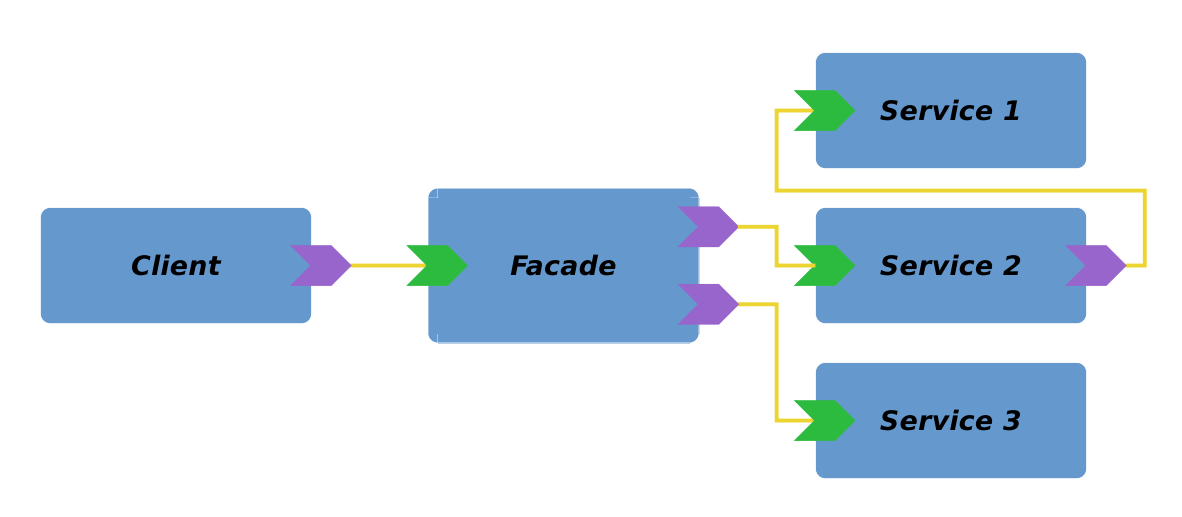
\includegraphics[scale=0.2]{media/facade.png}

\caption{Le patron facade \citep{Demange2013}\label{facade}.}

\end{center}

\end{figure}


\red{Pour d\'etecter un patron fa�ade, une des m\'ethodes consiste \`a calculer son temps de r\'eponse et son ratio de couplage entrant sur le couplage sortant.
Une fa�ade devrait avoir un fort temps de r\'eponse puisqu'elle offre un point d'entr\'ee au syst\`eme \`a de nombreux clients et un faible ratio couplage entrant / sortant puisqu'elle cache l'impl\'ementation de nombreux autres services \citep{Demange2013}.
}




\section{D\'etection d'anti-patrons SOA}


Contrairement aux patrons SOA, les anti-patrons ont beaucoup moins \'et\'e \'etudi\'es par la communaut\'e.
En effet, \red{la litt\'erature sur le sujet est plut\^ot r\'eduite}.
De ce fait, la plupart des r\'ef\'erences sont des pages Internet o� des d\'eveloppeurs SOA partagent leurs exp\'eriences sur les bonnes pratiques SOA  \citep{LubaCherbakovMamdouhIbrahim2005}.
Il existe tout de m\^eme quelques ouvrages cons\'equents, notamment \citep{Dudney2003} qui constitue le premier livre sur les anti-patrons SOA.
Cet ouvrage r\'epertorie 53 anti-patrons li\'es \`a l'architecture et l'impl\'ementation de syst\`emes JEE (\textit{Java 2 Platform Enterprise Edition}), tels que les EJB (\textit{Enterprise Java Beans}, JSP (\textit{JavaServer Pages}) ou encore les \textit{Servlets}.
Malgr\'e la pertinence de ce livre pour nos recherches, il ne propose aucune approche pour la d\'etection automatique de ces patrons.
\red{De plus, ces anti-patrons sont uniquement applicables aux syst\`emes JEE alors que la plupart d'entre eux ne sont que des variantes des \textit{Tiny Servic}e et \textit{Multi Service} \'evoqu\'es dans l'introduction.
} Kral et Zemkicka ont eux aussi apport\'e une contribution significative aux anti-patrons SOA.
En effet, ils ont sp\'ecifi\'e sept anti-patrons SOA directement li\'es \`a l'utilisation de pratiques objets.
Une fois encore, la question de la d\'etection automatique de ces anti-patrons n'est pas \'evoqu\'ee \citep{Kral2009}.


Bien que le catalogue global d'anti-patrons SOA commence \`a gagner un certain int\'er\^et et grossit de jour en jour, seulement de quelques contributions existent pour la d\'etection automatique d'anti-patrons dans des environnements SOA.
En effet, seulement deux contributions sont \`a signaler \citep{Eck2009} en plus de la n�tre --- SODA --- d\'ecrite dans trois publications diff\'erentes \citep{Moha, Nayrolles, Palma}.
D'autres auteurs proposent une technique pour d\'ecouvrir des anti-patrons d\'ependant des flux de donn\'ees, comme par exemple, des donn\'ees manquantes, inconsistantes ou encore supprim\'ees trop t�t.
Ils d\'etectent ces anti-patrons sp\'ecifiques en analysant les d\'ependances entre les donn\'ees dans les flux d'ex\'ecution et les probl\`emes qui pourraient appara�tre en cas de manipulation non optimale \citep{Eck2009}.
Cette \'etude, bien que pertinente pour nos recherches, se concentre sur les anti-patrons SOA li\'es aux flux de donn\'ees alors que nous cherchons \`a d\'etecter les anti-patrons SOA distribu\'es dans tout le syst\`eme et non reli\'e \`a une activit\'e particuli\`ere.




\section{SODA, l'approche de l'\'etat de l'art pour la d\'etection automatique d'anti-patrons SOA\label{soda}.}


Comme mentionn\'e plus haut, l'unique approche automatique disponible pour la d\'etection d'anti-patrons SOA est SODA \citep{Moha, Nayrolles, Palma}.
SODA repose sur un langage de r\`egles qui permet la sp\'ecification d'anti-patrons en utilisant un ensemble de m\'etriques.
Un processus g\'en\'erique transforme les sp\'ecifications en algorithmes de d\'etection \`a ex\'ecuter sur les syst\`emes \`a analyser.
SODA est compos\'e des trois \'etapes d\'ecrite ci-apr\'es et illustr\'ees  par la figure \ref{fig:The-SODA-approach}:


\begin{figure*}


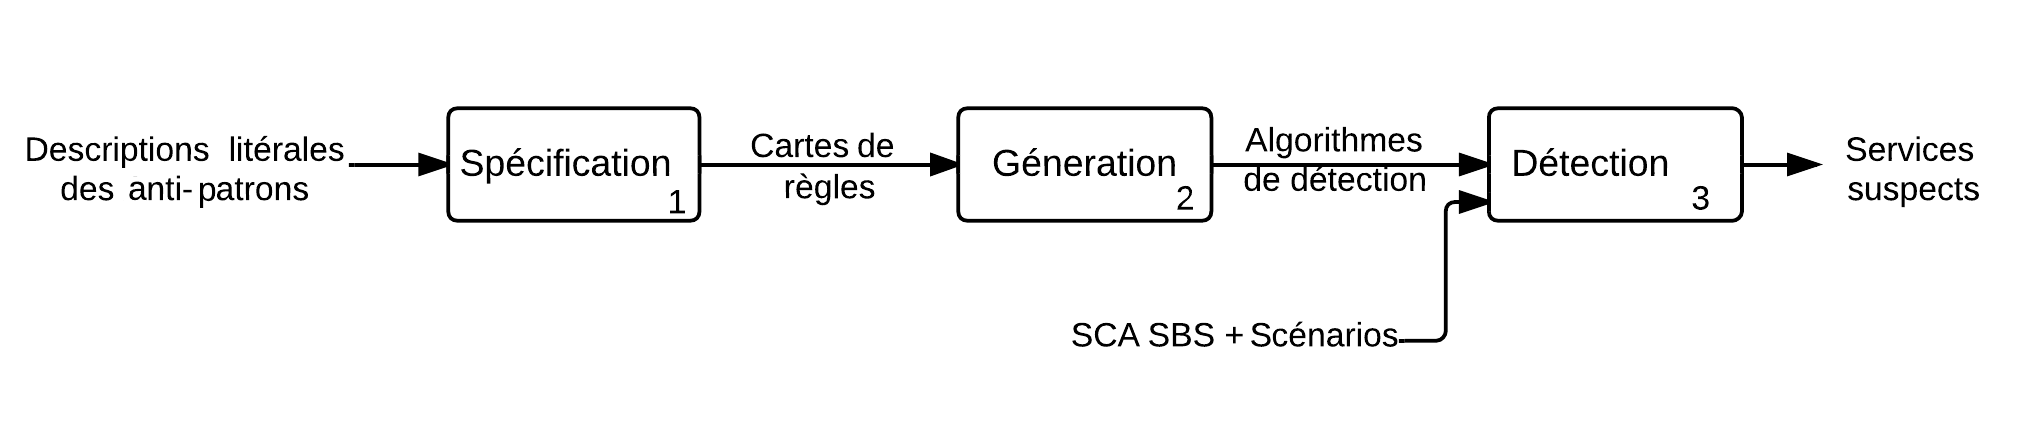
\includegraphics[scale=0.21]{media/SODA.png}%


\caption{\label{fig:The-SODA-approach}L'approche SODA}

\end{figure*}



\textit{Sp\'ecification d'anti-patrons SOA:} Cette \'etape identifie les propri\'et\'es relevant de la sp\'ecification des anti-patrons SOA.
Ces descriptions textuelles sont pr\'esent\'ees dans le tableau \ref{tab:List-of-SOA}.
Les propri\'et\'es correspondent de mani\`ere g\'en\'erale \`a des m\'etriques, par exemple, la coh\'esion, le couplage, le nombre de m\'ethodes, le temps de r\'eponse et la disponibilit\'e.
De plus, ces propri\'et\'es sont utilis\'ees comme base d'un DSL, qui prend la forme d'un langage \`a base de r\`egles pour la sp\'ecification d'anti-patrons SOA.
La sp\'ecification finale est une \textit{carte de r\`egles}, qui est une composition de r\`egles combinant des m\'etriques.



\begin{longtable}{p{.95\textwidth}}

\tabularnewline

\hline 

\textbf{Multi-Service}, aussi connu sous le nom  ``God object'' dans le paradigme objets,
correspond \`a un service qui impl\'emente une \textbf{multitude de m\'ethodes} faisant r\'ef\'erence \`a diff\'erentes abstractions m\'etiers et techniques.
Il agr\`ege beaucoup d'abstractions diff\'erentes \`a l'int\'erieur d'un un m\^eme service.
Un tel service est difficilement r\'eutilisable \`a cause de la \textbf{faible coh\'esion} entre ses m\'ethodes et il est souvent non disponible aux utilisateurs finaux \`a cause de sa charge, laquelle peut introduire de fort temps de r\'eponse \citep{Dudney2003}.


\begin{center}

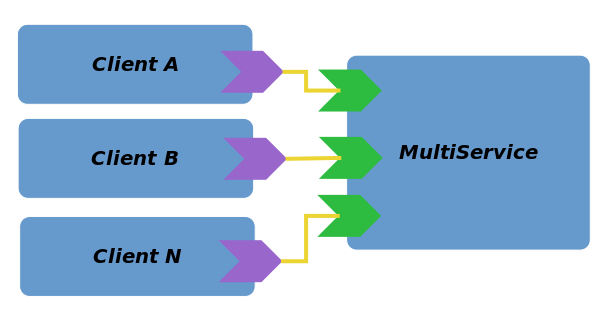
\includegraphics[scale=0.3]{media/multisca.png}

\end{center}

\vspace{-0.5cm}

\tabularnewline

Le \textbf{Tiny Service} est un petit service avec \textbf{peu de m\'ethodes} qui impl\'ementent uniquement une partie d'une abstraction.
Un tel service requiert plusieurs services coupl\'es pour \^etre utilis\'e correctement.
De ce fait, le Tiny Service introduit une complexit\'e importante dans le d\'eveloppement.
Dans certains cas extr\^eme, le Tiny Service est limit\'e \`a \textbf{une m\'ethode unique}, avec pour cons\'equence de nombreux services impl\'ementant l'ensemble des fonctionnalit\'es sous-jacentes \citep{Dudney2003}.


\begin{center}

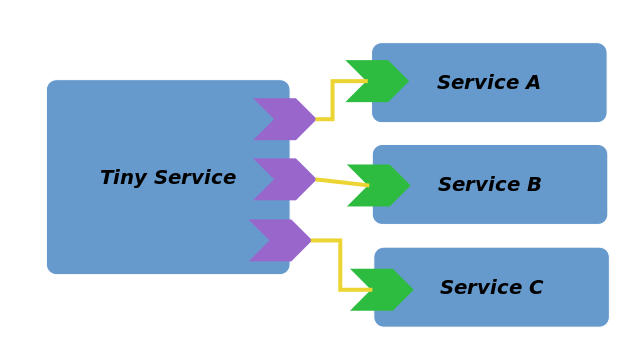
\includegraphics[scale=0.3]{media/Tinysca.png}

\end{center}

\vspace{-0.5cm}

\tabularnewline

Le \textbf{Chatty Service} correspond \`a un service qui \textbf{\'echange beaucoup de donn\'ees} de type primitif.
Le Chatty Service est aussi caract\'eris\'e par un \textbf{grand nombre d'invocations}; il \textit{discute} \'enorm\'ement avec le reste du syst\`eme \citep{Dudney2003}.


\begin{center}

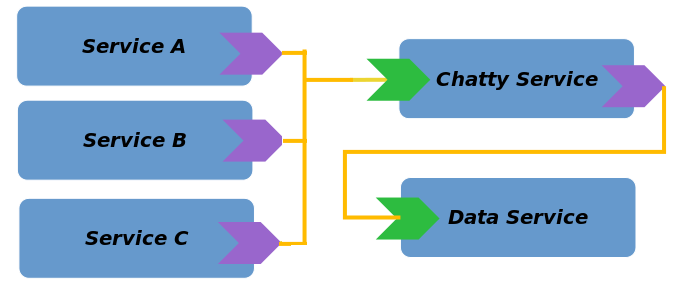
\includegraphics[scale=0.3]{media/chattysca.png}

\end{center}

\vspace{-0.5cm}

\tabularnewline

Le \textbf{Knot} est un ensemble de services \textbf{tr\`es peu coh\'esifs} et \textbf{fortement coupl\'es entre eux}.
Ces services sont de ce fait, tr\`es difficilement r\'eutilisables.
\`A cause de la complexit\'e induite de l'architecture, la disponibilit\'e de ces services peut \^etre faible et leur temps de r\'eponse \'elev\'e \citep{Rotem-Gal-Oz2012}.


\begin{center}

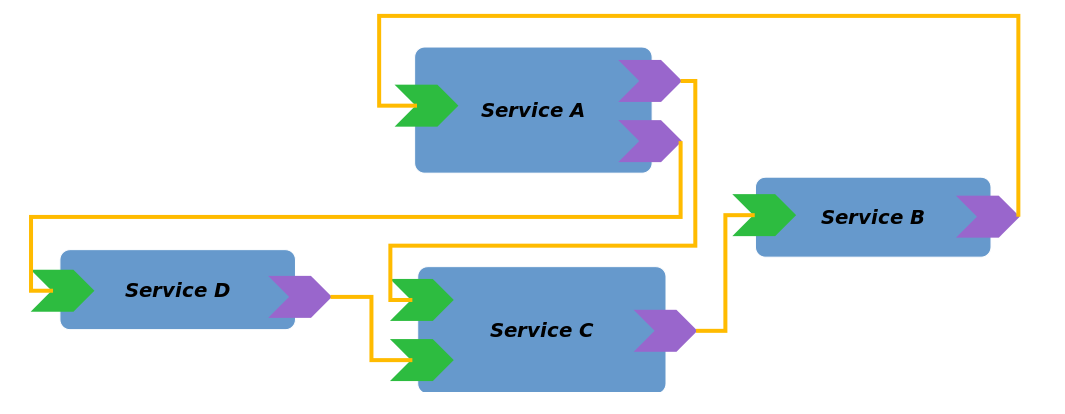
\includegraphics[scale=0.3]{media/knotsca.png}

\end{center}

\vspace{-0.5cm}

\tabularnewline

Le \textbf{Bottleneck Service} est un service \textbf{tr\`es utilis\'e} par le reste du syst\`eme (les autres services ou clients).
Il a un \textbf{fort couplage entrant et sortant}.
Son temps de r\'eponse peut \^etre \'elev\'e car il est utilis\'e par de nombreux clients, et les clients doivent attendre la r\'eponse des couches inf\'erieures.
De plus, sa disponibilit\'e peut \^etre faible \`a cause du trafic engendr\'e.


\begin{center}

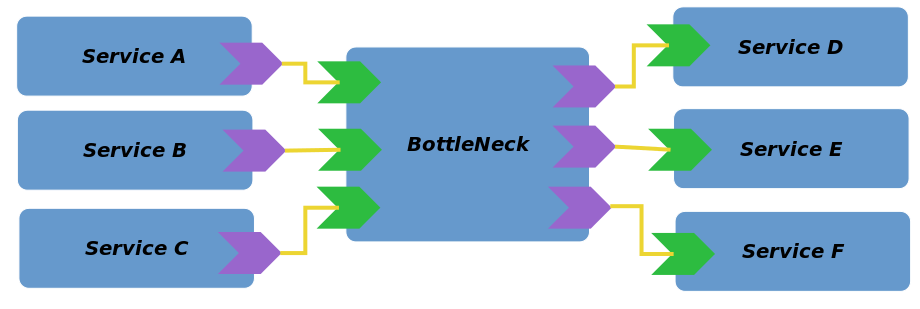
\includegraphics[scale=0.3]{media/bottlesca.png}

\end{center}

\vspace{-0.5cm}

Le \textbf{Service Chain}, aussi connu sous le nom de ``Message Chain'' dans les syst\`emes objets, correspond \`a \textbf{une cha�ne de services}.
Le Service Chain appara�t quand la requ\^ete d'un client est compl\'et\'ee par une invocation cons\'ecutive et successive de services.
Ce genre de \textbf{cha�nes de d\'ependances} engendrent des \textbf{invocations transitives}.


\begin{center}

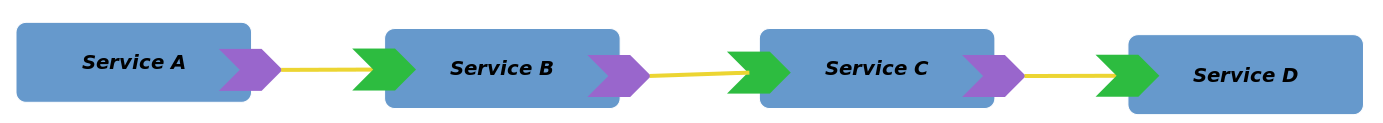
\includegraphics[scale=0.28]{media/chainsca.png}

\end{center}

\vspace{-0.5cm}

\tabularnewline

\hline 

\caption{Anti-patrons SOA \citep{Moha} \label{tab:List-of-SOA}.}

\end{longtable}


\textit{G\'en\'eration des algorithmes de d\'etection:} Le but de cette \'etape est de g\'en\'erer automatiquement des algorithmes de d\'etection en visitant les cartes de r\`egles sp\'ecifi\'ees \`a l'\'etape pr\'ec\'edente.
Ce processus est automatique et g\'en\`ere des algorithmes de d\'etection directement ex\'ecutables.



\textit{D\'etection des anti-patrons SOA:} Cette troisi\`eme et derni\`ere \'etape consiste \`a appliquer les algorithmes g\'en\'er\'es sur un syst\`eme \`a base de services.
Cette \'etape permet la d\'etection automatique des anti-patrons SOA en utilisant un ensemble de sc\'enarios pr\'ed\'efinis qui invoquent les interfaces des services.
\`A la fin de cette \'etape, les services du syst\`eme suspect\'es d'\^etre impliqu\'es dans un anti-patron SOA sont identifi\'es.



Bien qu'efficace et pr\'ecis, SODA est une approche intrusive, car elle requiert un ensemble de sc\'enarios qui invoquent concr\`etement les interfaces des services du syst\`eme.
De plus, son analyse dynamique implique des propri\'et\'es propres aux syst\`emes SCA (\textit{Service Component Architecture}, une sourcouche au SOA).
En effet, l'analyse dynamique de SODA repose sur le tissage d'aspects qui est une fonctionnalit\'e de la programmation orient\'ee aspects qui consiste \`a ins\'erer du code, qui s'ex\'ecutera avant ou apr\`es une m\'ethode donn\'ee,  dans le code m\'etier de l'application vis\'ee.
SCA est la seule technologie SOA \`a supporter cette fonctionnalit\'e.



\section{Conclusion}


De nombreux travaux ont \'et\'e men\'es pour la d\'etection d'anti-patrons dans les syst\`emes orient\'es objets, notamment les approches d\'erivant ou am\'eliorant celle de \citep{Moha2010}.
Pour le monde des applications \`a base de services, la communaut\'e a cr\'e\'e un catalogue tr\`es dense de patrons SOA, mais une seule approche vise leur d\'etection dans le but de d\'eterminer la qualit\'e globale du syst\`eme pour faciliter la maintenance et l'\'evolution de tels syst\`emes.
Cette approche pr\'esent\'ee par \textit{Demange et al.} a \'et\'e inspir\'ee par une autre approche nomm\'ee SODA -- que nous avons propos\'ee en 2012 \citep{Moha, Nayrolles, Palma}.
SODA se concentre, elle aussi, sur la facilitation de la maintenance et de l'\'evolution des applications \`a base de services, mais en d\'etectant les anti-patrons SOA.
Malgr\'e que ces deux approches soient pertinentes et efficaces, elle sont limit\'ees par plusieurs points:


\begin{itemize}

\item Elles n\'ecessitent d'avoir un bon niveau de contr�le sur le syst\`eme analys\'e;
en particulier elles doivent avoir acc\`es aux interfaces des services du syst\`eme;

\item Elles n\'ecessitent de poss\'eder des sc\'enarios pertinents;

\item SODA est majoritairement bas\'e sur des m\'etriques statiques alors que
SODOP utilise une part plus importante de m\'etriques dynamiques;

\item Techno-centrique (SCA) puisque bas\'e sur le tissage d'aspects.


\end{itemize}


Notre objectif est de reprendre les forces de ces approches comme la sp\'ecification d\'eclarative des anti-patrons via un language d\'edi\'e et la g\'en\'eration automatique d'algorithmes de d\'etection.
N\'eanmoins, nous voulons nous abstraire de la technologie du syst\`eme analys\'e, en nous appuyant sur des donn\'ees qui refl\`etent la nature hautement dynamique des SBSs.
Nous souhaitons aussi \'eviter toute intrusion dans le fil d'ex\'ecution normal du syst\`eme vis\'e.


\chapter{\'Etat de l'art sur l'extraction de connaissances � partir de traces d'ex�cution}

Les traces d'ex�cution sont � la base de la majorit� des analyses dynamiques de syst�mes complexes.
Les traces d'ex�cution peuvent �tre collect�es gr�ce � l'ex�cution normale -- en opposition � l'ex�cution contr�l�e ou dirig�e -- du syst�me analys�.
Cependant, les traces d'ex�cution sont r�put�es �tre difficiles � appr�hender � cause de la quantit� consid�rable de donn�es qu'elles contiennent.
En effet, l'ex�cution d'un syst�me de taille moyenne peut potentiellement produire des millions de traces, chacune �tant une composition d'information telle que l'horodatage (\textit{timestamp} en anglais), l'identification du client ou du sous-syst�me courant.
Au fil des ann�es, des techniques du domaine de la fouille de donn�es ont �t�  appliqu�es aux traces d'ex�cution afin d'en extraire des informations int�r�ssantes.

Dans ce chapitre couvrant l'�tat de l'art de l'extraction de connaissances � partir de traces d'ex�cution, nous allons, dans un premier temps, faire une revue des travaux portant sur l'extraction de connaissances dans des environnements orient�s services.
Dans un second temps, nous introduirons les notions de fouille de r�gles d'association classiques et s�quentielles.

\section{Extraction de connaissances depuis des traces d'ex�cution}

Un nombre important d'�tudes se sont concentr�es sur l'extraction des connaissances contenues dans les traces d'ex�cution.
Ces �tudes ont �t�s motiv�es par l'identification d'aspects \citep{Tonella}, de processus d'affaires \citep{Khan2010}, de patrons d'utilisation de services \citep{Asbagh2007}, et l'identification de fonctionnalit�s � la fois dans les syst�mes orient�s objets \citep{Dustar2006} et services \citep{Safyallah2006}.
 Tonella et Cecetato (2004) ont identifi� les aspects en g�n�rant des traces  li�es � l'ex�cution des principales fonctionnalit�s d'un syst�me.
 Ensuite, ces traces d'ex�cution sont compar�es aux unit�s du syst�me qui ont �t� utilis�es --- ce qui induit un contr�le sur le code source --- via l'analyse formelle de concepts.
Le treillis r�sultant permet de d�tecter les diff�rents aspects de l'application  \citep{Tonella}.
Khan \textit{et al.} (2010) fouillent les processus d'affaires dans un environnement SOA en identifiant les traces relatives � un processus.
Ces traces appel�es "traces de processus" sont ensuite soumises � de nombreuses conversions et analyses s�mantiques afin d'en retirer les diff�rents processus d'affaires \citep{Khan2010}.
\citet{Asbagh2007} fouillent des patrons d'ex�cution s�quentiels dans les s�quences d'utilisation de services dans le but d'en extraire des patrons d'utilisation g�n�raux et proposent un algorithme performant pour cette t�che sp�cifique.

Une �tude particuli�rement importante, car proche de notre approche, porte sur l'identification de composition de services \citep{Upadhyaya2012a}, c'est-\`a-dire, des services qui sont utilis�s ensemble de fa�on r�p�t�e tout en �tant structurellement et fonctionnellement similaires.
 Les auteurs d�tectent neuf compositions de services en utilisant l'analyse de traces d'ex�cution et l'algorithme Apriori (voir section \ref{apriori}) pour les d�tecter.
 Ils identifient aussi les patrons de composition qui sont structurellement ou fonctionnellement proches afin de les repr�senter � un niveau d'abstraction sup�rieur.

Un petit nombre de projets ont explor� la d�tection de patrons de conception bas�e sur la fouille de traces.
\citet{Ng2010} ont propos� MoDeC, une approche pour identifier des patrons de conception comportementaux et de cr�ation en utilisant une analyse dynamique et de la programmation par contraintes.
Ils ont r�alis� une r�tro-ing�nierie des sc�narios d'utilisation en instrumentant le \textit{bytecode}\footnote{Le \textit{bytecode} est un code interm�diaire, plus concret (plus proche des instructions machines) que le code source, qui n'est pas directement ex�cutable.
Il est contenu dans un fichier binaire qui repr�sente un programme, tout comme un fichier objet produit par un compilateur.} et ont appliqu� des techniques de programmation par contraintes pour d�tecter des patrons de collaboration � l'ex�cution.
\citet{Hu2008} se sont attaqu�s � la d�tection de patrons de conception dans les traces d'ex�cution en utilisant des sc�narios, de la fouille de patrons et de l'analyse formelle de concepts.
Leur approche est guid�e par un ensemble de sc�narios uniques par fonctionnalit� de l'application afin d'identifier des patrons par fonctionnalit�.


Bien que diff�rentes dans leurs buts et �tendues, les �tudes pr�sent�es ci-dessus portant sur des anti-patrons et patrons orient�s objets forment une base d'expertise  et de savoir technique pour cr�er de nouvelles m�thodes visant la d�tection d'anti-patrons SOA.
Malgr� le nombre important de ressemblances, les techniques de d�tection pour les anti-patrons objets ne peuvent pas �tre directement appliqu�es pour les services.
En effet, les syst�mes orient�s services utilisent les services comme bloc de construction et, de ce fait, se placent � une abstraction sup�rieure � l'objet.
De plus, la nature hautement dynamique et distribu�e des syst�mes � base de services soul�ve des d�fis qui ne sont pas pr�pond�rants dans les syst�mes objets.
De mani�re g�n�rale, ces d\'efis sont li�s � des difficult�s � �tablir l'ordre des �v�nements, tout comme le comportement stochastique dont de tels syst�mes sont capables.
De ce fait, les techniques �tablies pour le paradigme objet ne peuvent pas �tre appliqu�es.


\section{Introduction � la fouille de r�gles d'association\label{ARM}}

Dans le domaine de la fouille de donn�es, la fouille de r�gles d'association (\textit{Association rule Mining}, ARM) est une m�thode reconnue pour d�couvrir des co-occurrences entre les attributs d'objets dans des bases de donn�es colossales \citep{Gregory1991}.
Les r�gles d'association classiques sont repr�sent�es par $A \rightarrow B$, o� A et B sont des ensembles d'attributs.
En d'autre mots, la fouille de r�gles d'association cherche � extraire --- depuis un ensemble de transactions compos�es d'items --- les items qui apparaissent souvent ensemble (itemsets fr�quents) et des r�gles ant�c�dent $\rightarrow$ cons�quent pr�disant l'occurrence d'un item d'apr�s les occurrences d'autre items dans la transaction (r�gles d'association).

La force d'une r�gle est mesur�e par une m�trique de \textit{confiance}.
La confiance mesure la fr�quence de B dans les transactions ayant d�j� A (Equation \ref{confidentce}).
Dans cette �quation  $\sigma (A \cup B)$ repr�sente le nombre d'apparitions de A et B dans la m�me transaction et $\sigma (A)$ le nombre de transaction dans lesquelles A appara�t.

\begin{equation}\label{confidentce}
\textit{Confiance (A entraine B)} =  \frac{\sigma (A \cup B)}{\sigma (A)}
\end{equation}

L'importance de la r�gle, quant � elle, c'est-\`a-dire, combien de fois le motif correspondant apparara�t dans les traces, est mesur�e par le \textit{support} (Equation \ref{Support}).
Dans cette seconde �quation, la signification de $\sigma (A \cup B)$ est identique et $|T|$ est le nombre de transactions.

\begin{equation}\label{Support}
\textit{Support (A entraine B)} = \frac{\sigma (A \cup B)}{|T|}
\end{equation}

Pour s'assurer qu'uniquement les r�gles avec un fort potentiel d'information soient retenues, la fouille est encadr�e par des seuils  minimaux � atteindre pour les deux m�triques.

\subsection{L'algorithme Apriori\label{apriori}}

L'algorithme Apriori -- publi� en 1994 -- est, probablement, l'algorithme le plus populaire pour extraire de telles r�gles d'association \citep{Agrawal1994}.
Voici un aper�u de son mode op�ratoire.
Pour chaque transaction ($t \in T$) du tableau~\ref{transaction}, nous prenons en compte chaque article achet� sans pr�occupation de quantit�.


\begin{table}[h!]
\centering
\scriptsize
\begin{tabular}{|c|c|}
\hline
Transaction & Items\\
\hline
\hline
1 & Pain, Lait\\
2 & Pain, Couche, Bi�re, Oeufs\\
3 & Lait, Couche, Bi�re, Coke \\
4 & Pain, Couche, Lait, Bi�re \\
5 & Coke, Lait, Pain, Couche \\
\hline
\end{tabular}
\caption{Table de transactions.\label{transaction}}
\end{table}

Ensuite, l'algorithme g�n�re les ensembles d'items par taille et ce en
fonction d'un support minimum. Ici le support $supp(x)  = \frac{\sigma (x)}{|T|}$ repr�sente la fr�quence d'apparition de l'itemset $(it)$ dans l'ensemble des transactions $(T)$.
Le r�sultat de cette op�ration est pr�sent� par le tableau \ref{itmf}.
Par exemple, l'article \{Pain\} est pr�sent dans quatre des cinq transactions.
Il a donc un support de 80\%.
Les itemssets fr�quents peuvent aussi �tre compos�s de plusieurs articles; par exemple ``Bi�re'' et ``Couche'' apparaissent dans trois des cinq transactions donc \{Bi�re, Couche\} a un support de 60\%.

\begin{table}[h!]
\centering
\scriptsize
\begin{tabular}{|c|c|c|}
\hline
Itemsets fr�quents & Support\\
\hline
\hline
\{Pain\} & 80\% \\
\{Lait\} & 80\% \\
\{Couche\} & 80\% \\
\{Bi�re\} & 60\% \\
\{Pain, Lait\} & 60\% \\
\{Pain, Couche\} & 60\% \\
\{Bi�re, Couche\} & 60\% \\
\{Lait, Couche\} & 60\% \\
\hline
\end{tabular}
\caption{Itemsets fr�quents avec un support minimum de 50\%\label{itmf}.}
\end{table}

A partir de ces itemsets fr�quents, l'algorithme g�n�re les r�gles d'association, en suivant et
en restreignant les r�sultats en fonction de certaines valeurs comme la confiance.
Des exemples de r�gles d'association sont pr�sent�s par le tableau \ref{ar}.
Si nous prenons l'itemset fr�quent \{Bi�re, Couche\} qui dispose de 60\% de support (trois des cinq transactions), nous remarquons qu'il est aussi associ� � l'article ``Lait'' dans deux des trois transactions.
Nous pouvons donc �crire que \{Bi�re, Couche\} $\rightarrow$ \{Lait\} avec un support de 40\% car cette r�gle appara�t dans deux des cinq transactions et avec une confiance � 67\% car \{Bi�re, Couche\} appara�ssent trois fois mais ne sont accompagn�s par \{Lait\} que deux fois.

\begin{table}[h!]
\centering
\scriptsize
\begin{tabular}{|c|c|c|}
\hline
R�gles & Support & Confiance\\
\hline
\hline
\{Lait,Couche\} $\rightarrow$ \{Bi�re\} & 40\% & 67\% \\
\{Lait,Bi�re\} $\rightarrow$ \{Couche\} & 40\% & 100\% \\
\{Bi�re, Couche\} $\rightarrow$ \{Lait\} & 40\% & 67\% \\
\{Bi�re\} $\rightarrow$ \{Lait,Couche\} & 40\% & 67\%  \\
\{Couche\} $\rightarrow$ \{Lait,Bi�re\} & 40\% & 50\% \\
\{Lait\} $\rightarrow$ \{Couche,Bi�re\} & 40\% & 50\%\\
\hline
\end{tabular}
\caption{Exemples de r�gles fouill�es depuis le tableau \ref{itmf}\label{ar}.}
\end{table}

\section{R�gles d'association s�quentielles}

 Bien que les r�gles d'association classiques aient pu nous apporter des informations pertinentes, nous sommes int�ress�s par la pr�servation des s�quences d'invocation de services.
 De ce fait, nous avons adopt� une variante, ``\textit{les r�gles d'association s�quentielles}'' dans laquelle, $ A $ et $B$ deviennent des s�quences d'�v�nements (achet� par un m�me client, alarmes r�seaux, ou tout autre sorte d'�v�nements g�n�raux).
 De plus, dans notre cas les s�quences suivent un ordre temporel dans le sens o� la partie gauche (ant�c�dent) se produit avant la partie droite (cons�quent).
 Les r�gles qui peuvent �tre d�couvertes depuis les traces d'ex�cution mettent au premier plan des informations cruciales � propos de la chance de voir appara�tre des services ensemble dans les traces d'ex�cution et dans un ordre sp�cifique.
 Ainsi, une r�gle d'association s�quentielle peut ressembler � :
\begin{center}
$ServiceA,~ServiceB~implique~ServiceC$ 
\end{center}
qui signifie qu'apr�s l'ex�cution du service A suivi de celle du service B, il y a de bonnes chances de voir le service C appara�tre.
Dans un souci de clart�, nous avons limit� la taille de l'ant�c�dent et du cons�quent, n�anmoins, les deux c�t�s de la r�gle peuvent �tre des s�quences de taille arbitraire.


\subsection{L'algorithme RuleGrowth}

\textit{RuleGrowth} est un algorithme r�cent --- publi� en 2011 --- qui vise la d�couverte de r�gles d'association s�quentielles dans de larges bases de donn�es \citep{Fournier-viger2011}.
Plus sp�cifiquement, RuleGrowth se focalise sur des s�quences compos�es d'�v�nements ordonn�s dans le temps.
Cependant, les �v�nements peuvent aussi �tre regroup�s en ensemble d'�v�nements.
Dans ce cas ci, les �v�nements sont consid�r�s comme simultan�s.

\begin{table}[h!]
\centering
\scriptsize
\begin{tabular}{|c|c|}
\hline
ID & Items \\
\hline
\hline
1 & \{Clean Code\},\{Refactoring\};\{Clean Coder\};\{Design Patterns, Refactoring to Patterns\}\\ \hline
\multirow{3}{*}{2} & \{Clean Code, Clean Coder\};\{Refactoring, Design Patterns\};\{Head First DP\}\\
& \{Head First DP, Refactoring to Patterns\};\{Clean Code, Refactoring\} \\ 
& \{Clean Coder, Refactoring to Patterns\};\{Design Patterns\} \\ \hline
\multirow{2}{*}{3} & \{Head First DP\};\{Patterns of Enterprise Apps\};\{Clean Code, Refactoring to Patterns\} \\ 
& \{Refactoring\};\{Design Patterns\}\\ \hline
\end{tabular}
\caption{Base de donn�es de s�quences d'achat de livres\label{seq}.}
\end{table}

Dans le tableau \ref{seq}, nous pouvons observer trois s�quences diff�rentes compos�es d'ensembles d'�v�nements identifi�s par des accolades et s�par�s par des virgules.
Lorsque l'on souhaite pr�dire ce qui va se passer � la suite d'�v�nements, nous pouvons utiliser les r�gles d'association s�quentielles qui, comme vu dans la section \ref{ARM}, sont de la forme $ A \rightarrow B$, signifiant que B a des chances de se produire apr�s A.
De telles r�gles ont �t� utilis�es dans de nombreux domaines: l'analyse de cours boursier \citep{Yang2006} ou l'�tablissement de pr�visions m�t�orologiques \citep{Ho2005}.

En utilisant les s�quences du tableau \ref{seq}, RuleGrowth est capable d'extraire les r�gles pr�sent�es par le tableau \ref{rulesSample}.

\begin{table}[h!]
\centering
\scriptsize
\begin{tabular}{|c|}
\hline
R�gles  \\
\hline
\hline
Clean Code $\Rightarrow$ Refactoring \\
Clean Code $\Rightarrow$ Refactoring, Design Patterns \\
Clean Code $\Rightarrow$ Design Patterns \\
Clean Code, Refactoring $\Rightarrow$ Design Patterns \\
Clean Code, Refactoring,Clean Coder $\Rightarrow$ Design Patterns \\
Clean Code, Refactoring,Head First DP $\Rightarrow$ Design Patterns \\
Clean Code, Refactoring, Head First DP, Refactoring to Patterns \\
Clean Code, Refactoring, Refactoring to Patterns $\Rightarrow$ Design Patterns \\
Clean Code, Clean Coder $\Rightarrow$ Design Patterns \\
Clean Code, Head First DP $\Rightarrow$ Design Patterns \\
Clean Code, Head First DP, Refactoring to Patterns $\Rightarrow$ Design Patterns \\
\hline
\end{tabular}
\caption{Exemples de r�gles d'association s�quentielles.\label{rulesSample}}
\end{table}

RuleGrowth surclasse les autres algorithmes existants -- CMRules et CMDeo \citep{Fournier-Viger2012} -- car il utilise des techniques �labor�es afin de g�n�rer beaucoup moins de candidats et, par cons�quent, �tre plus performant.

\section{Conclusion}

De nombreuses �tudes ont vis� l'extraction de donn�es interpr�t�es depuis les traces d'ex�cution et certaines d'entre elles ont, avec succ�s, extrait toutes sortes de patrons pour repr�senter le syst�me sous analyse.
Nous avons propos� une introduction � un sous-domaine de la fouille de donn�es --- dont l'�tude des traces d'ex�cution d�pend --- nomm� la fouille de r�gles d'association et plus particuli�rement la fouille de r�gles d'association s�quentielles via deux algorithmes.
La fouille de r�gles d'association classique ou non s�quentielle dans les traces d'ex�cution g�n�r�es par des syst�mes � base de services a d�j� �t� explor�e par \citep{Upadhyaya2012a}.
 Dans cette �tude, les auteurs proposent une approche pour la d�couverte de patrons de composition.
 N�anmoins, ils ne tiennent pas compte de l'ordonnancement des appels ce qui autorise la g�n�ration de plus de r�gles et en r�duit donc leur pertinence.
La technique de la fouille de r�gles d'association s�quentielles sera utilis�e dans notre approche d�crite dans le chapitre suivant.
\chapter{L'approche SOMAD}

Dans ce chapitre, nous pr�sentons l'approche SOMAD (\textit{Service Oriented Mining for Antipatterns Detection}), compos�e de cinq �tapes, pour la d�tection d'anti-patrons bas�e sur les traces d'ex�cution produites par les syst�mes � base de services.
Cette nouvelle approche est une variante de SODA \citep{Nayrolles,Moha} bas�e sur les traces d'ex�cution.
Les traces peuvent provenir de n'importe quelles impl�mentations SOA.
SODA est applicable uniquement sur des syst�mes SCA en utilisant un ensemble de sc�narios pr�d�finis.
Plus particuli�rement, dans SOMAD, nous sp�cifions un nouvel ensemble de m�triques qui s'appliquent sur des r�gles d'association s�quentielles extraites depuis les traces d'ex�cution.
La figure~\ref{fig:The-SOMAD-approach} montre une vue d'ensemble de SOMAD.
Les nouvelles �tapes correspondantes � SOMAD sont en gris tandis que celles de SODA sont en blanc.
La premi�re �tape \textit{(\'Etape 1.Inf�rence de m�triques)} est support�e par la cr�ation d'hypoth�ses provenant de la description textuelle des anti-patrons SOA.
Ces hypoth�ses sont utilis�es dans cette �tape pour inf�rer de nouvelles m�triques d�di�es � l'interpr�tation de r�gles d'association s�quentielles.
La seconde �tape \textit{(\'Etape 4.Fouille de r�gles d'association)} a pour but d'extraire les r�gles d'association des traces d'ex�cution du syst�me � base de services vis�.
Les r�gles d'association s�quentielles sugg�rent des relations int�ressantes entre les services dans de larges amas de traces d'ex�cution.


\begin{figure*}

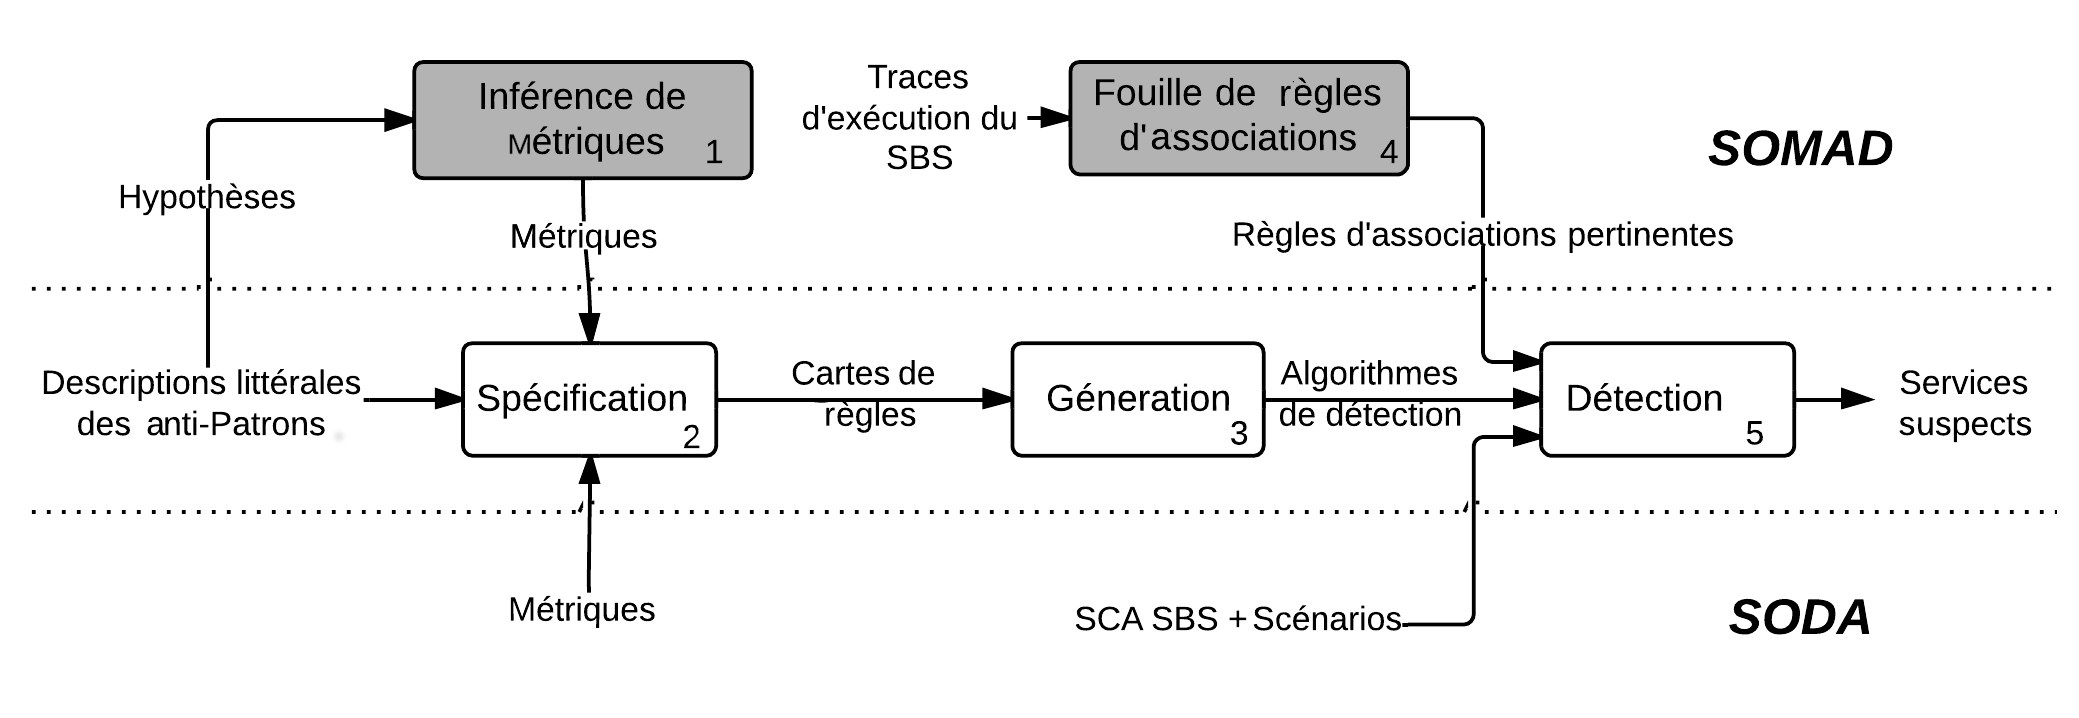
\includegraphics[scale=0.20]{media/SOMAD.png}%

\caption{\label{fig:The-SOMAD-approach}Les approches SODA et SOMAD.
Les cases grises correspondent aux nouvelles �tapes de SOMAD ajout�es aux �tapes de SODA en blanc.}
\end{figure*}


\section{\'M�thodologie de SOMAD}

Dans cette section nous pr�sentons toutes les �tapes SOMAD.

\subsection{\'Etape 1. Inf�rence de m�triques} Un ensemble de m�triques d�di�es � l'interpr�tation de r�gles s�quentielles d'association est inf�r� depuis trois hypoth�ses construites via la description textuelle des anti-patrons (tableau \ref{tab:List-of-SOA}).
\blue{Tel que pr�sent� par la figure \ref{infmetric}, cette �tape a comme entr�e des hypoth�ses bas�es sur les descriptions textuelles des anti-patrons et produit des m�triques.}

\begin{figure}[h]
\begin{center}
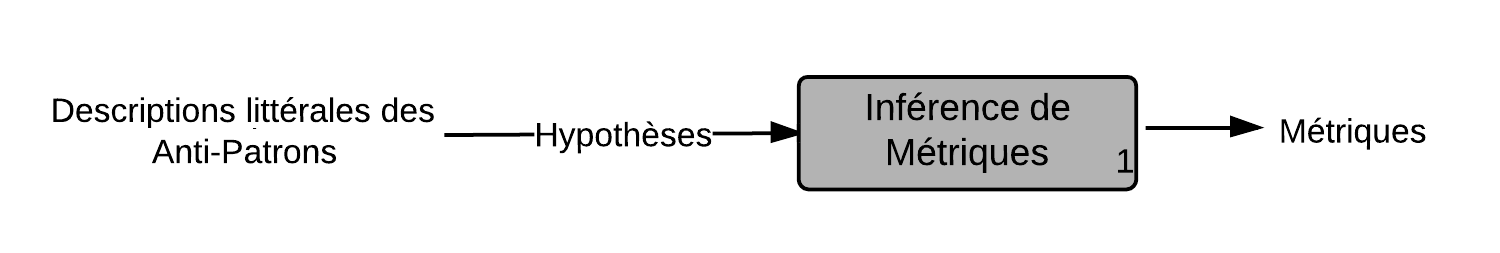
\includegraphics[scale=0.25]{media/step1.png}
\end{center}
\caption{\'Etape 1: Inf�rence de m�triques.\label{infmetric}}
\end{figure}


Ces hypoth�ses correspondent � des heuristiques qui permettent l'interpr�tation de r�gles d'association s�quentielles dans le but d'identifier les propri�t�s pertinentes des anti-patrons SOA.
Apr�s une �tude minutieuse des descriptions textuelles des anti-patrons, nous constatons que les anti-patrons SOA peuvent �tre sp�cifi�s en termes de couplage et de coh�sion.
Le couplage fait r�f�rence au degr� de d�pendance entre les services tandis que la coh�sion repr�sente la coh�rence des responsabilit�s pr�sent�es par un service \citep{Perepletchikov2007, Perepletchikov2010}.

\begin{hypothesis}
\label{cpl}
Si un service A implique un service B avec un fort support et une grande confiance, alors A et B sont fortement coupl�s.
\end{hypothesis}

\begin{hypothesis}
\label{ocpl}
Si un service apparait en tant que cons�quent (ant�c�dent) d'un grand nombre de r�gles d'association s�quentielles, alors il a un fort couplage entrant (sortant).
\end{hypothesis}

Les hypoth�ses \ref{cpl} et \ref{ocpl} qualifient le couplage entre deux services et le couplage g�n�ral en termes de couplage entrant et de couplage sortant.

La coh�sion est aussi largement utilis�e dans les descriptions textuelles des anti-patrons, de ce fait, nous l'avons prise en compte dans l'hypoth�se \ref{coh}.

\begin{hypothesis}
\label{coh}
Si le nombre de m�thodes d'un service donn� est similaire au nombre de ses diff�rents partenaires (Hypoth�se \ref{ocpl}, le nombre de services avec qui il communique), alors le service n'est pas coh�sif.
\end{hypothesis}

En se basant sur les trois hypoth�ses ci-dessus, nous avons cr�� des m�triques sp�cifiques au domaine afin d'explorer les manifestations d'anti-patrons SOA cach�es dans les r�gles d'association s�quentielles.
Afin de mieux comprendre comment nous passons des hypoth�ses aux m�triques, la figure \ref{tiny-sample} donne un exemple pour le \textit{Tiny Service}.
Nous pouvons voir que le Tiny Service est caract�ris� par deux de nos trois hypoth�ses (Hypoth�ses 3.1 et 3.3) et ces hypoth�ses ont �t�s traduites en deux m�triques distinctes nomm�es OC (\textit{Outgoing Coupling}) et NM (\textit{Number of Methods}).

\begin{figure}[h]
\begin{center}
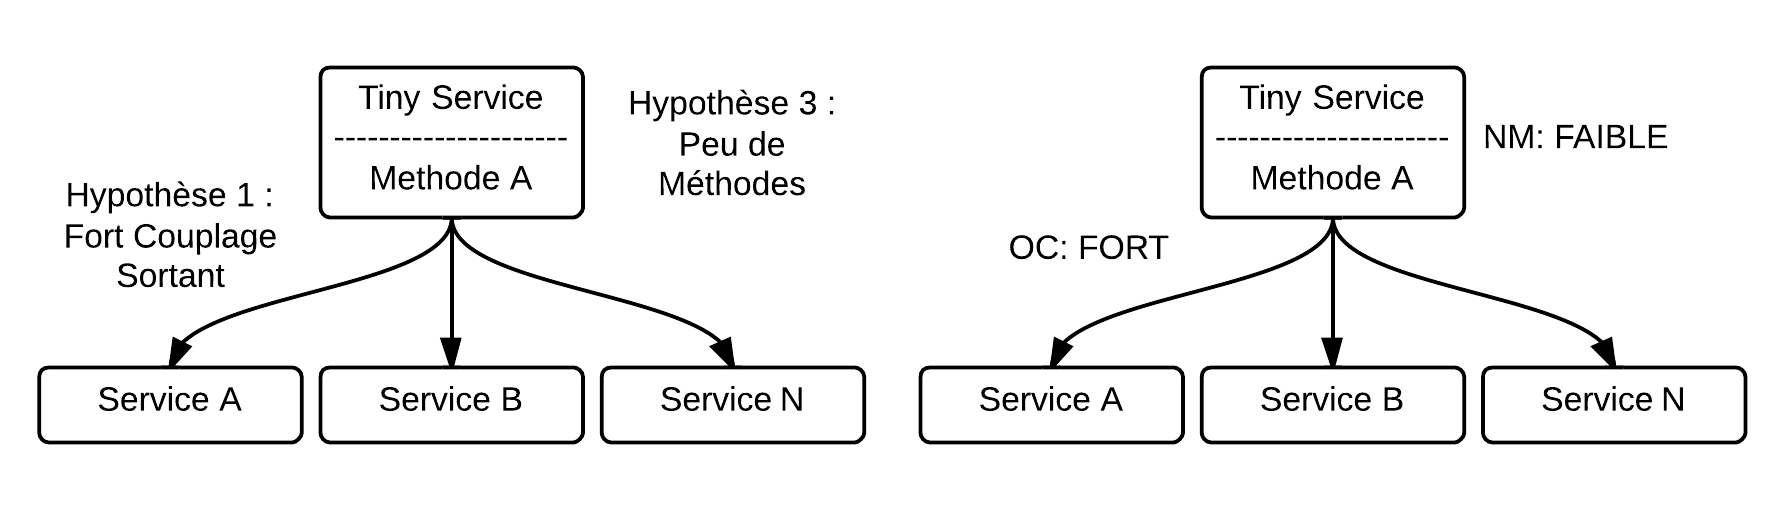
\includegraphics[scale=0.2]{media/Tiny-example.png}
\end{center}
\caption{Exemple de l'utilisation des hypoth�ses et m�triques: Le \textit{Tiny Service}\label{tiny-sample}.}
\end{figure}

Les m�triques que nous avons con�ues et impl�ment�es sp�cifiquement pour supporter SOMAD et qui seront utilis�es pour cr�er des cartes de r�gles gr�ce � un DSL (\textit{Domain Specific Language}) sont pr�sent�es par les tableaux \ref{MetricsS} et \ref{MetriquesC}.
Dans ces tableaux, des notations math�matiques standards ont �t� utilis�es lorsque possible et �tendues (ajout de symboles non standards) quand n�cessaire.
Les r�gles d'association peuvent �tre visualis�es par (X $\rightarrow$ Y) avec X et Y respectivement l'ant�c�dent et le cons�quent d'une r�gle.
\emph{K, L} sont les services partenaires.
$AR$ repr�sente l'ensemble complet des r�gles d'association, tandis que $AR_{s}$
et $AR_{m}$ repr�sente respectivement les sous-ensembles relatifs aux r�gles d'association au niveau service et au niveau m�thode.
\emph{$M_{S}$} d�note les m�thodes d'un service donn� $S$.
Finalement, nous utilisons des symboles non-standards pour les s�quences d'op�rations: $[ ]$ est le constructeur de s�quences, $\Cup$ signifie concat�n� (\textit{append} en anglais) dans la s�quence; $\Subset$ repr�sente les sous-s�quences d'une relation; et A $\lessdot$ B veut dire que le service A appara�t dans la s�quence B.


\begin{table}
\begin{tabular*}{14cm}
{@{\extracolsep{\fill}}p{14cm}}
\hline 
\textbf{\emph{Number of Matches (NMA(S))}}\textbf{ }: $\#\{X\rightarrow Y\in AR_{s}\mid S\lessdot(X\Cup Y)\}$
\} 
\tabularnewline
\hline 
Compte le nombre de r�gles dans lesquelles un service appara�t; que ce soit en tant qu'ant�c�dent ou cons�quent.
\tabularnewline
\hline 
\hline 
\textbf{\emph{Number of Diff.
Partners (NDP(S))}} :\\
$\#\{K\mid X\rightarrow Y\in AR_{s},S\lessdot X,K\lessdot Y\}$
$+\#\{K\mid X\rightarrow Y\in AR_{s},S\lessdot Y,K\lessdot X\}$
\tabularnewline
\hline 
Indique combien de partenaires a un service.
En d'autres mots, cette m�trique d�termine si le service communique avec beaucoup d'autres services ou non.
 \tabularnewline
\hline 
\hline 
\textbf{\emph{Incoming Coupling (IC(S)) }}: $\sum_{L\in\{K\mid X\rightarrow Y\in AR_{s},K\lessdot X,S\lessdot Y\}}\frac{CID(S,X)}{NDP(S)}$ \tabularnewline
\hline 
Compte le nombre de fois o� un service est utilis�.
Cependant, au lieu de compter de mani�re classique l'apparition du service, nous utilisons une valeur contextuelle: $\frac{CID(S,X)}{NDP(S)}$ o� X est le service partenaire.
Ainsi, le couplage est inversement proportionnel au nombre de partenaires diff�rents.
\tabularnewline
\hline 
\hline 
\textbf{\emph{Outgoing Coupling (OC(S)) }}: $\sum_{L\in\{K\mid X\rightarrow Y\in AR_{s},S\lessdot X,K\lessdot Y\}}\frac{CID(X,S)}{NDP(S)}$ \tabularnewline
\hline 
Les m�mes principes s'appliquent que ceux vus pour l'\textit{Incoming Coupling}.
Cette m�trique compte le nombre de fois o� le service vis� utilise d'autres services.
\tabularnewline
\hline 
\hline 
\textbf{\emph{Number of Methods (NM(S))}} : $\#\{K\mid X\rightarrow Y\in AR_{m},K\in M_{s},K\lessdot(X\Cup Y)\}$\tabularnewline
\hline 
Compte le nombre de m�thodes diff�rentes expos�es dans les r�gles d'association s�quentielles.
Cette m�trique porte uniquement sur le sous-ensemble $AR_{m}$.
\tabularnewline
\hline 
\hline 
\textbf{\emph{Cohesion (COH(S)) : }}$\frac{NDP(S)}{NM(S)}$ \tabularnewline
\hline 
Fournit un ratio comprenant le nombre de partenaires diff�rents et le nombre de m�thodes disponibles.\tabularnewline
\hline 
\end{tabular*}

\caption{M�triques simples\label{MetricsS}.}


\end{table}

\begin{table}
\begin{tabular*}{14cm}
{@{\extracolsep{\fill}}p{14cm}}
\hline 
\textbf{\emph{Cross Invocation Dependencies (CID($S_{a},S_{b}$))}}
: \\ $\#\{X\rightarrow Y\in AR_{s}\mid S_{a}\lessdot X,S_{b}\lessdot Y\}$
$+\#\{X\rightarrow Y\in AR_{s}\mid S_{a}\lessdot Y,S_{b}\lessdot X\}$ \tabularnewline
\hline 
Cette m�trique est cruciale pour la d�tection des manifestations enfouies dans les traces.
En effet, elle explore les interactions typiques entre les services tout en ignorant les interactions non fr�quentes (d� au seuil � atteindre, voir section \ref{ARM}).
Pour obtenir cette information, CID compte toutes les r�gles d'association o� un service $a$ ($S_a$) est pr�sent dans la partie des ant�c�dents et un service $b$ (S$_b$) dans la partie des cons�quents ou vice et versa.
\tabularnewline
\hline 
\hline 
\textbf{\emph{Transitive Coupling (TC$(S_{a},S_{b})$)}} : \\
$\#\{K\mid X\rightarrow Y\in AR_{s},S_{a}\lessdot X,S_{b}\lessdot Y,({[S_{a},K]\Subset X}\vee[K,S_{b}]\Subset Y)\}$\tabularnewline
\hline 
Transitive Coupling a �t� b�tie pour d�tecter un anti-patron SOA particulier, le \textit{Service Chain} (voir \ref{tab:List-of-SOA}).
Tout d'abord, nous avons observ� qu'une paire de services qui ne communiquent pas directement ne veut pas pour autant dire que les services ne sont pas coupl�s.
Ceci est l'id�e fondatrice du \textit{Service Chain} et de cette m�trique.
Afin d'identifier le couplage transitif dans les r�gles d'association, ce qui est beaucoup plus difficile que le couplage direct, nous avons besoin de repr�senter une cha�ne dans les r�gles d'association.
Un service $a$ ($S_a$) est dans l'ant�c�dent d'une r�gle et un service $b$ ($S_b$) est dans le cons�quent d'une autre r�gle.
Ces deux r�gles sont connect�es gr�ce � un service $k$ ($S_k$) qui apparait dans le cons�quent de la premi�re r�gle et dans l'ant�c�dent de la seconde r�gle.
Ainsi, dans un cas trivial, nous pourrions avoir :{[}a{]}$\rightarrow${[}b{]}
et {[}b{]}$\rightarrow${[}c{]}.
Dans cette configuration, a et c ne sont pas directement coupl�s mais si c est indisponible, il y a de bonnes chances pour que a et b le soient \'egalement.
Des chaines de distance sup�rieur � 3 sont �galement possibles.
\tabularnewline
\hline 
\end{tabular*}

\caption{M�triques complexes\label{MetriquesC}.}


\end{table}

\subsection{\'Etape 2. Sp�cification d'anti-patrons SOA} Les m�triques d�finies � l'�tape 1 nous permettent de sp�cifier des anti-patrons SOA sous la forme de carte de r�gles.
 Afin de combiner ces m�triques, nous avons utilis� un DSL d�fini par \citep{Moha} et qui a ensuite �t� perfectionn� par \citep{Demange2013} ainsi que \citep{Nayrolles}.
Ce DSL est pr�sent� dans la figure \ref{fig:BNF} sous la forme d'une grammaire Backus-Naur.
Une r�gle d�crit une m�trique, une relation, ou une combinaison d'autres r�gles (ligne 3) en utilisant un ensemble d'op�rateurs (ligne 6).
Les m�triques qui sont disponibles apparaissent ligne 11.
Une m�trique peut �tre d�finie comme une combinaison d'autres m�triques (lignes 9 et 10).
Chaque m�trique peut �tre compar�e � une ou plusieurs valeurs ordinales (ligne 7) -- un ensemble de cinq valeurs de l'�chelle de Likert \citep{MichaelS.1971} de tr�s faible (\textit{very low}) � tr�s fort (\textit{very high}) --  ou �tre compar�es � une valeur num�rique (ligne 8) en utilisant des comparateurs (ligne 13).

\begin{figure*}
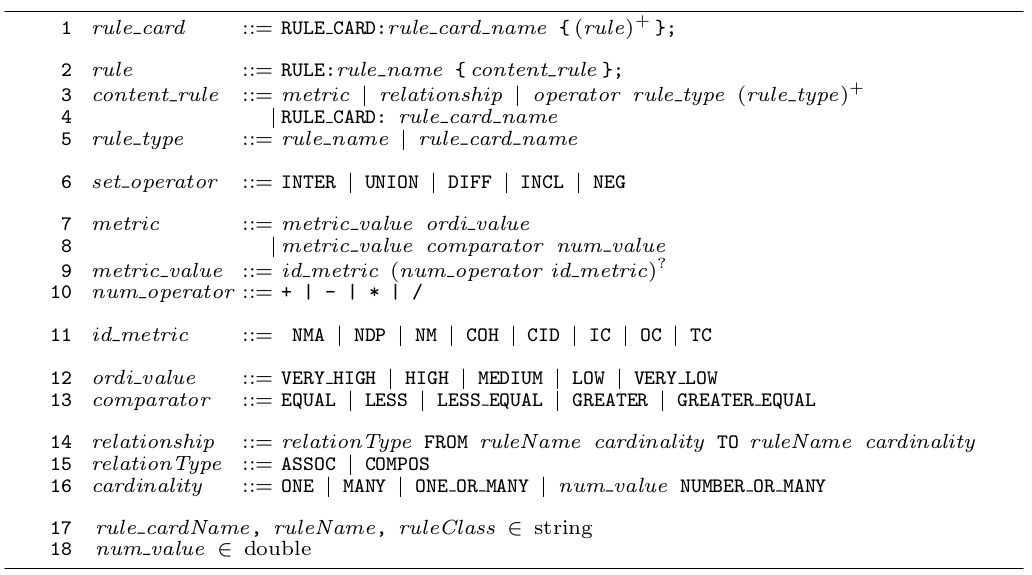
\includegraphics[scale=0.38]{media/BNF.png}%
\caption{\label{fig:BNF} Grammaire BNF utilis�e pour construire les cartes de r�gles.}
\end{figure*}

\blue{La figure \ref{specstep} pr�sente les entr�es de cette seconde �tape, � savoir les descriptions textuelles des anti-patrons ainsi que les m�triques issues de l'�tape 1.
Cette �tape de sp�cification produit des cartes de r�gles.}


\begin{figure}[h]
\begin{center}
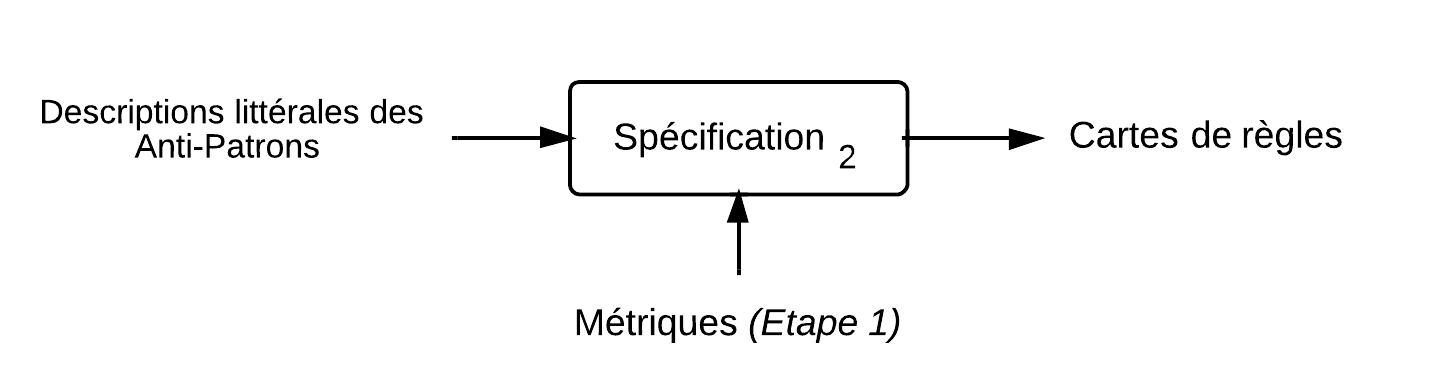
\includegraphics[scale=0.25]{media/step2.png}
\end{center}
\caption{\'Etape 2: Sp�cification d'anti-patrons SOA.\label{specstep}}
\end{figure}

Les cartes de r�gles utilis�es pour sp�cifier les anti-patrons SOA sont pr�sent�es par la figure \ref{fig:rules}.
A titre d'exemple, la carte de r�gles correspondant au \textit{Tiny Service} (figure \ref{fig:rules}-b) est compos�e de trois r�gles.
La premi�re (ligne 2) est une intersection de deux r�gles (lignes 3 et 4) qui d�finissent deux m�triques: un fort couplage sortant (\textit{Outgoing Coupling OC}) et un faible nombre de m�thodes (\textit{Number of Methods NM}).

\begin{figure}
\begin{small}
\scriptsize
1~RULE\_CARD:~\emph{\textbf{MultiService}}~\{\\
2~~RULE:~\emph{\textbf{MultiService}}\{INTER~\emph{\textbf{LowCohesion}}~\emph{\textbf{ManyMethods}}~\emph{\textbf{ManyMatches}}\};\\
3~~RULE:~\emph{\textbf{LowCohesion}}\{COH~LOW\};\\
4~~RULE:~\emph{\textbf{ManyMethods}}\{NM~HIGH\};\\
5~~RULE:~\emph{\textbf{ManyMatches}}\{NMA~HIGH\};\\
6~\};
\vspace{-0.2cm}
\begin{center}
(a) Multi Service
\end{center}
\vspace{-0.2cm}
1~RULE\_CARD:~\emph{\textbf{TinyService}}~\{\\
2~~RULE:~\emph{\textbf{TinyService}}\{INTER~\emph{\textbf{HighOutgoingCoupling}}~\emph{\textbf{FewMethods}}\};\\
3~~RULE:~\emph{\textbf{HighOutgoingCoupling}}\{OC~HIGH\};\\
4~~RULE:~\emph{\textbf{FewMethods}}\{NM~LOW\};\\
5~\};
\vspace{-0.2cm}
\begin{center}
(b) Tiny Service
\end{center}
\vspace{-0.2cm}
1~RULE\_CARD:~\emph{\textbf{ChattyService}}~\{\\
2~~RULE:~\emph{\textbf{ChattyService}}\{INTER~\emph{\textbf{ManyPartners}}~\emph{\textbf{ManyMatches}}\};\\
3~~RULE:~\emph{\textbf{ManyPartners}}\{NDP~VERY HIGH\};\\
4~~RULE:~\emph{\textbf{ManyMatches}}\{NMA~VERY HIGH\};\\
5~\};
\vspace{-0.2cm}
\begin{center}
(c) Chatty Service
\end{center}
\vspace{-0.2cm}
1~RULE\_CARD:~\emph{\textbf{BottleNeck}}~\{\\
2~~RULE:~\emph{\textbf{BottleNeck}}\{INTER~\emph{\textbf{HighOutgoingCoupling}}~\emph{\textbf{HighIncomingCoupling}}\};\\
3~~RULE:~\emph{\textbf{HighOutgoingCoupling}}\{OC~HIGH\};\\
4~~RULE:~\emph{\textbf{HighIncomingCoupling}}\{IC~HIGH\};\\
5~\};
\vspace{-0.2cm}
\begin{center}
(d) BottleNeck Service
\end{center}
\vspace{-0.2cm}
1~RULE\_CARD:~\emph{\textbf{KnotService}}~\{\\
2~~RULE:~\emph{\textbf{KnotService}}\{INTER~\emph{\textbf{LowCohesion}}~\emph{\textbf{HighCrossInvocation}}\};\\
3~~RULE:~\emph{\textbf{LowCohesion}}\{COH~LOW\};\\
4~~RULE:~\emph{\textbf{HighCrossInvocation}}\{CID~HIGH\};\\
5~\};
\vspace{-0.2cm}
\begin{center}
(e) Knot Service
\end{center}
\vspace{-0.2cm}
1~RULE\_CARD:~\emph{\textbf{ServiceChain}}~\{\\
2~~RULE:~\emph{\textbf{ServiceChain}}\{\emph{\textbf{HighTransitiveCoupling}}\};\\
3~~RULE:~\emph{\textbf{HighTransitiveCoupling}}\{TC~HIGH\};\\
4~\};
\vspace{-0.2cm}
\begin{center}
(f) Service Chain
\end{center}
\end{small}
\vspace{-0.2cm}
\caption{Cartes de r�gles\label{fig:rules} pour nos anti-patrons.}
\end{figure}

\subsection{\'Etape 3. G�n�ration des algorithmes de d�tection} 

Depuis les sp�cifications des anti-patrons SOA d�crites avec la DSL, nous g�n�rons automatiquement les algorithmes de d�tection.
Nous utilisons maintenant Ecore \citep{Sciamma2013} et Acceleo \citep{Obeo2005} pour automatiser la g�n�ration des algorithmes.
\blue{La figure \ref{gen} expose les entr�es de cette �tape: les cartes de r�gles g�n�r�es � l'�tape 2 ainsi qu'un gabarit \texttt{Java}.
Cette �tape produit des algorithmes de d�tection directement ex�cutables.}

\begin{figure}
\begin{center}
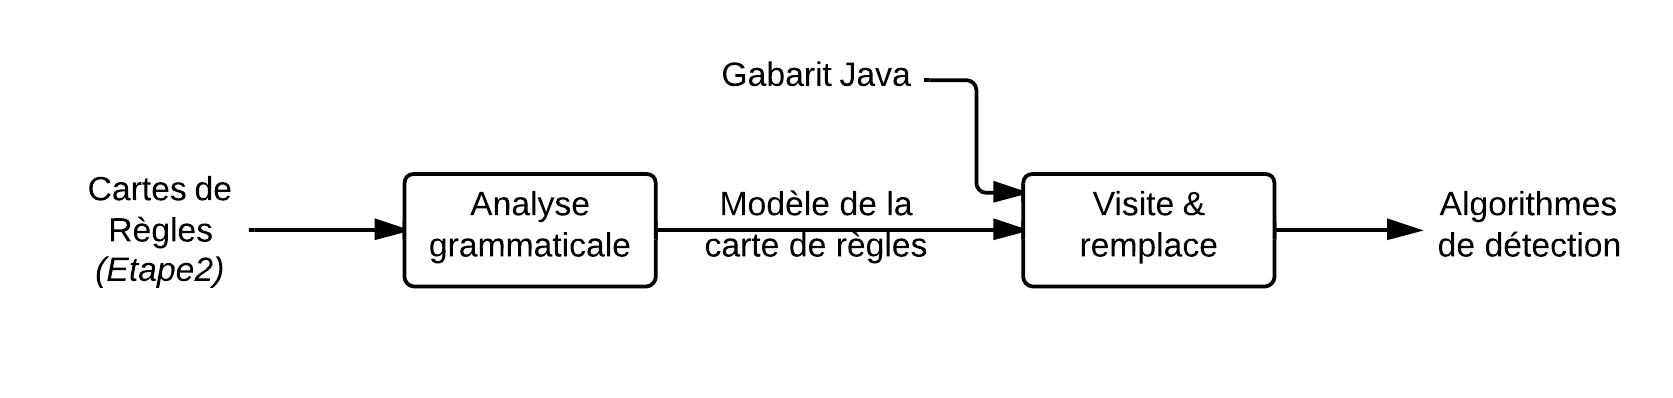
\includegraphics[scale=0.25]{media/step3.png}
\end{center}
\caption{\'Etape 3: G�n�ration d'algorithmes.\label{gen}}
\end{figure}

Pour la g�n�ration automatique des algorithmes de d�tection, nous commen�ons par analyser syntaxiquement (\textit{parser} en anglais) les \textit{cartes de r�gles} pour chaque anti-patron et nous les repr�sentons comme des mod�les.
Par la suite, nous utilisons Ecore pour les valider syntaxiquement par rapport au m�ta-mod�le de notre DSL.
Nous utilisons une g�n�ration de code automatique bas�e sur les mod�les et fournie par Acceleo \citep{Obeo2005}.
Pour ce faire, nous d�finissions un mod�le unique pour toutes les cartes de r�gles qui contient des \textit{�tiquettes}, qui seront par la suite, remplac�es par les m�triques d�finies dans la carte de r�gles.
Finalement, le mod�le unique est utilis� pour g�n�rer l'algorithme d'une carte de r�gles et produit une ou plusieurs classes Java, directement compilable et ex�cutable.


La figure \ref{template} montre le mod�le du \textit{Multi Service} que nous utilisons pour g�n�rer son algorithme de d�tection.
\`A la premi�re ligne de la figure \ref{template}, le mod�le importe le m�ta-mod�le de notre DSL.
Il contient aussi les \textit{tags}, qui sont identifiables par des crochets, et qui correspondent aux variables qui vont �tre remplac�es (\textit{rule card name}, \textit{rule names}, \textit{metrics}, \textit{values} et les diff�rents op�rateurs).
Un seul mod�le est requis pour toutes les cartes de r�gles.
Ainsi, il est ais� de les maintenir.

\begin{figure}
\begin{center}
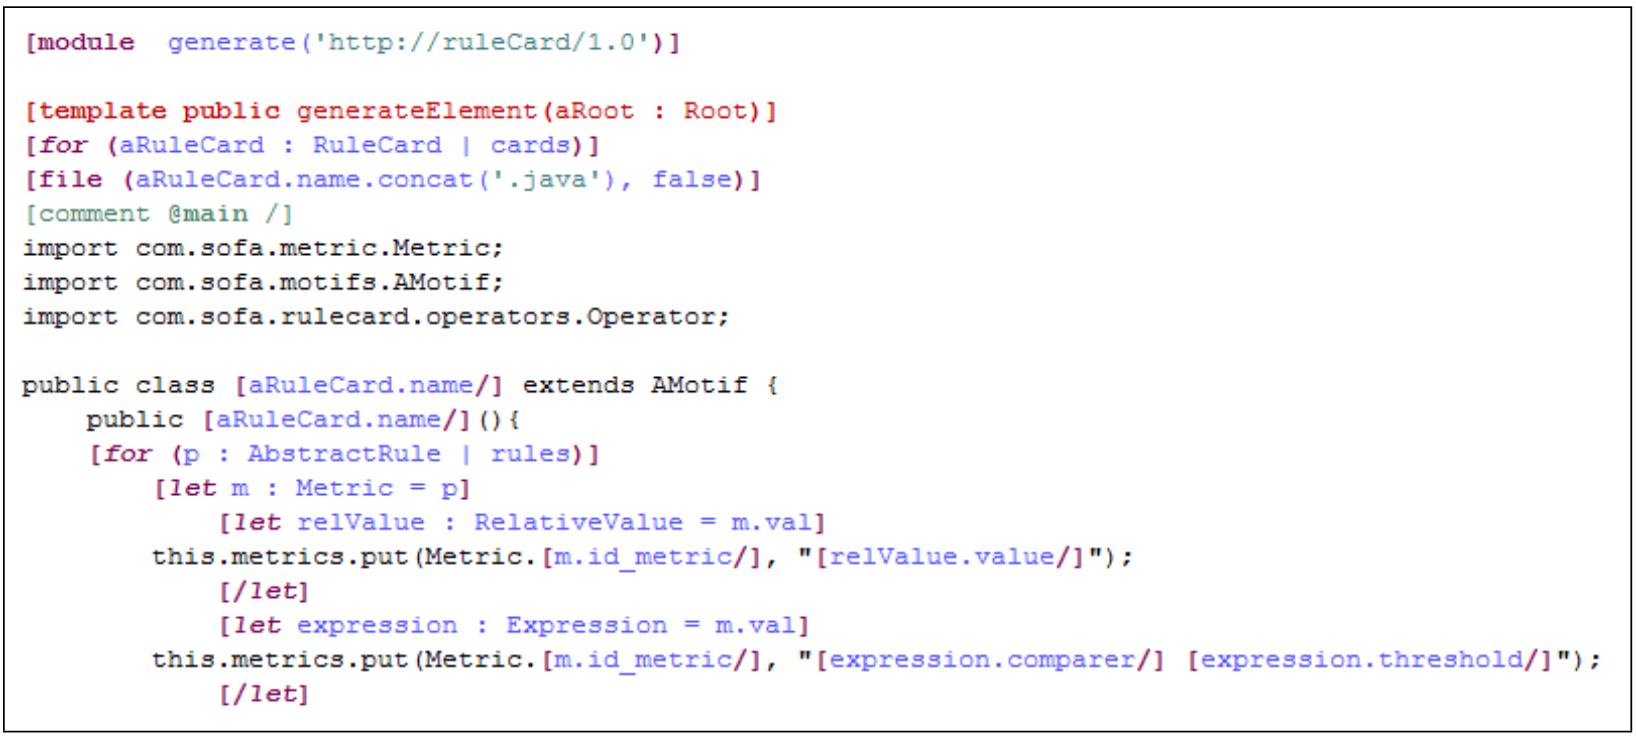
\includegraphics[scale=0.2]{media/template.png}
\end{center}
\caption{Gabarit pour la g�n�ration automatique\label{template}.}
\end{figure}

La figure \ref{code} montre le code g�n�r� par Acceleo.
Ce code est bas� sur la carte de r�gles de la figure \ref{template}.
Cette g�n�ration cr�e une classe Java avec les diff�rents op�rateurs et les diff�rentes m�triques.
La classe g�n�r�e est directement compilable et ex�cutable en utilisant un \textit{Java Class Loader}.
Les ing�nieurs n'ont plus qu'� fournir l'impl�mentation concr�te des m�triques qu'ils souhaitent utiliser.

\begin{figure}
\begin{center}
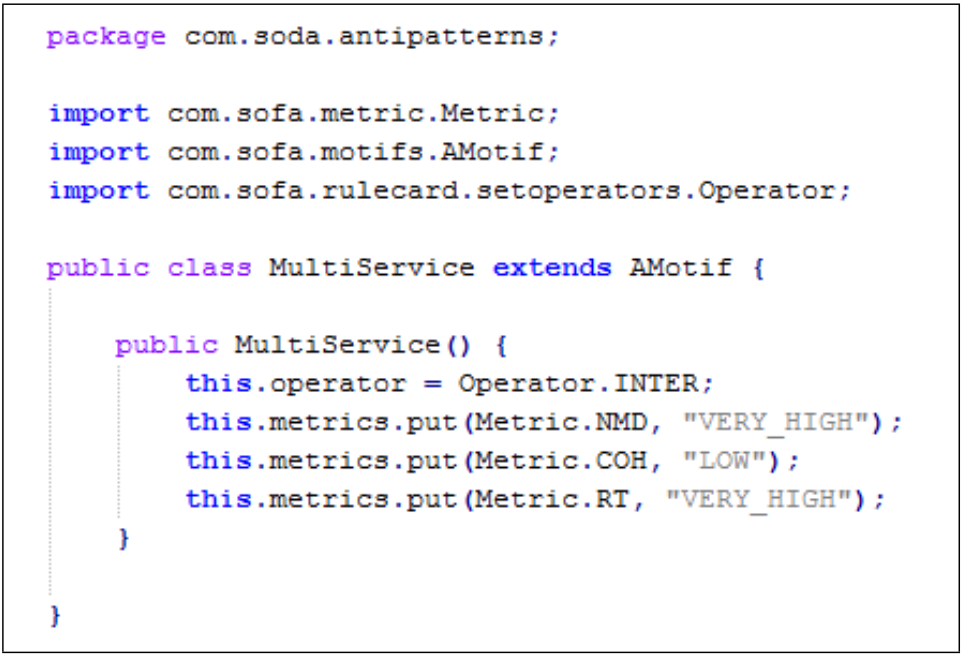
\includegraphics[scale=0.3]{media/multijava.png}
\end{center}
\caption{Capture d'�cran du code g�n�r�  pour le \textit{Multi-service.} \label{code}.}
\end{figure}

Ce processus est compl�tement automatis� pour �viter les t�ches manuelles qui sont source d'erreurs.
Ce processus garanti aussi la tra�abilit� entre la sp�cification des anti-patrons SOA faite avec la DSL et la d�tection qui sera effectu�e sur le syst�me � base de services.
De ce fait, les ing�nieurs logiciels peuvent se focaliser sur la sp�cification des anti-patrons, sans avoir � consid�rer les d�tails techniques de l'aggr�gation de r�gles et m�triques.

Nous pr�cisons aussi que, dans cette �tape, la g�n�ration automatique des algorithmes �tait d�j� pr�sente dans SODA et a �t� am�lior�e par Christopher Robert. 
Nous l'avons juste utilis�e afin de cr�er de nouveaux algorithmes compos�s de nos m�triques et capable de d�tecter des anti-patrons en interpr�tant les r�gles d'association s�quentielles.

\subsection{\green{\'Etape 4. Fouille des r�gles d'association}} Les traces d'ex�cution sont analys�es pour extraire les r�gles d'association s�quentielles.
\blue{Ce processus est illustr� par la figure \ref{fouille}.}

\begin{figure}
\begin{center}
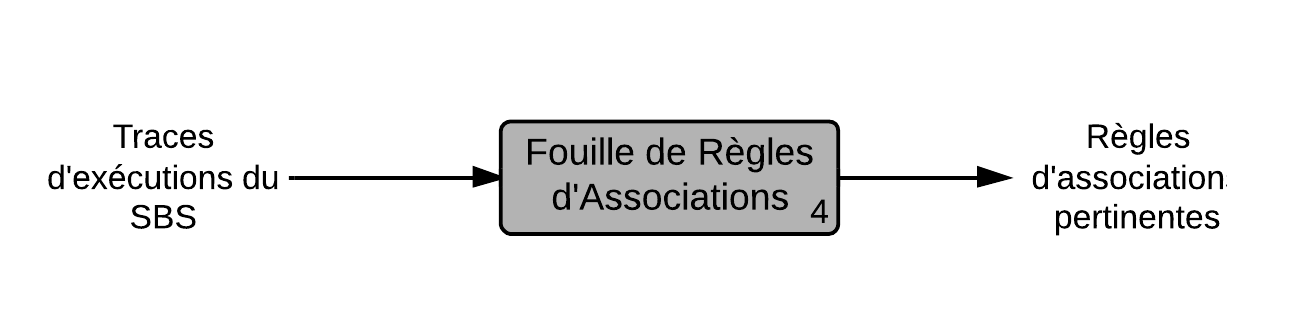
\includegraphics[scale=0.25]{media/step4.png}
\end{center}
\caption{\'Etape 4: Fouille de r�gles d'association.\label{fouille}}
\end{figure}


Les r�gles d'association s�quentielles sont fouill�es depuis une collection de traces d'ex�cution en utilisant un support et une confiance minimum.
Une transaction est un ensemble d'appels de services et de m�thodes ordonn�s dans le temps.
Nous rappelons que le support d'un patron\footnote{Dans le contexte des r�gles d'association; le mot \textit{patron} repr�sente un motif dans les traces d'ex�cution et non un patron de conception logiciel.}, c'est-\`a-dire, d'une s�quence d'items (appels de services ou m�thodes), est le pourcentage global de transactions qui contiennent ce patron. Quant � la confiance, elle mesure la vraisemblance que la partie cons�quente soit apr�s la partie ant�c�dente dans une m�me transaction.

Pour extraire les r�gles d'association s�quentielles, deux possibilit�s s'offraient � nous.
D'une part, la fouille de patron s�quentiel o� les algorithmes de fouille de r�gles ont �t� cr��s pour des structures l�g�rement plus g�n�rales que celles utilis�es ici.
Dans les faits, les patrons s�quentiels sont d�finis par des transactions qui repr�sentent des s�quences d'ensemble.
Des travaux int�ressants pour la d�couverte de patrons s�quentiels ont �t� publi�s, e.g, la m�thode PrefixSpan \citep{Mortazavi-Asl2004}.
D'autre part, les traces d'ex�cution ne contiennent pas r�ellement de pures transactions s�quentielles.
En effet, leur structure sous-jacente est compos�e d'�l�ments individuels.
De telles donn�es sont connues depuis le milieu des ann�es 90, cependant, elles ont re�u moins d'attention de la part de la communaut� de la fouille de donn�es; sans doute parcequ'elles sont moins int�r�ssantes � fouiller.
N�anmoins, de nombreuses applications pratiques ont �t� imagin�es dans des domaines o� ce genre de donn�es prolif�re, notamment dans la fouille de traces d'ex�cution de logiciel.
Dans la litt�rature g�n�rale de la fouille de donn�es, fouiller des s�quences pures, en opposition � la fouille de s�quence compos�es d'ensembles, a �t� trait�e par la fouille d'�pisodes \citep{Mannila1997}.
Les �pisodes sont compos�s d'�v�nements dans le sens o� un appel de service est un �v�nement.
Sans aucun doute, le domaine disposant de la plus grande base de connaissance sur le sujet est la fouille d'utilisation de site web.
Les donn�es d'entr�es sont � nouveau des traces d'ex�cution, n�anmoins cette fois les traces sont des requ�tes envoy�es � un serveur web \citep{Pei2000}.
Il est important de souligner que les patrons s�quentiels sont plus g�n�raux que ceux bas�s sur des s�quences pures.
En effet, les algorithmes de fouille qui ont �t� cr��s  pour les premiers peuvent �tre moins efficace que ceux cr��s pour les seconds car des �tapes suppl�mentaires peuvent �tre requises pour lister les ensembles significatifs.
N�anmoins, nous avons choisi d'utiliser un algorithme de fouille de patrons et r�gles s�quentielles qui, \green{malgr� les sp�cificit�s de nos donn�es --- compos�es d'�pisodes et non de s�quences --- f�t performant. Nous avons utilis� tout d'abord l'algorithme RuleGrowth \citep{Fournier-viger2011} qui semblait �tre le plus adapt� et a l'avantage d'�tre disponible gratuitement\footnote{\url{http://www.philippe-fournier-viger.com/spmf/}}}.
Bien que non optimis� pour les s�quences pures, ses performances sont plus que satisfaisantes.
Cependant, dans le prochain chapitre, nous pr�senterons une �volution de RuleGrowth nomm�e SOARuleGrowth qui est plus adapt�e � nos donn�es.
Pour r�sumer, � la fin de cette �tape, nous avons extrait les relations pertinentes entre les services.
Ces relations ont la forme de r�gles d'association s�quentielles.


La figure \ref{tinyR} pr�sente le processus de fouille de r�gles d'association s�quentielles dans les traces d'ex�cution appliqu� au \textit{Tiny Service}.
Dans les traces d'ex�cution, on constate que le Service A ne dispose que d'une seule m�thode, la m�thode A.
De plus cette m�thode fait appel aux services B, C ou D.
Ainsi, les r�gles d'association g�n�r�es pour cet ensemble de traces factices sont : A $\rightarrow$ B, A $\rightarrow$ C et A $\rightarrow$ D.

\begin{figure}
\begin{center}
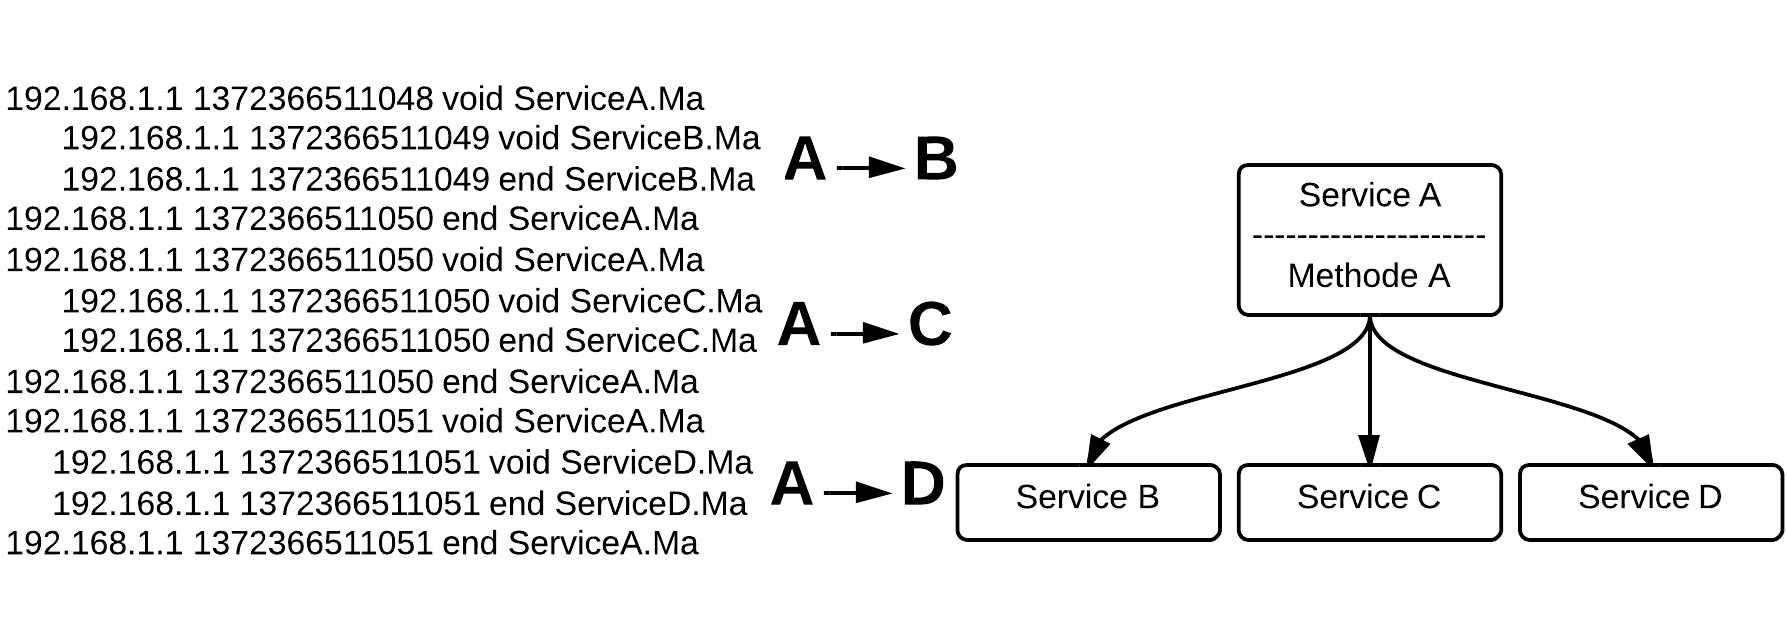
\includegraphics[scale=0.2]{media/Tiny-rules.png}
\end{center}
\caption{Fouille de r�gles d'association depuis les traces d'ex�cution: \textit{Le Tiny Service}.\label{tinyR}}
\end{figure}

\subsection{\'Etape 5. D�tection d'anti-patron SOA} 

Cette derni�re �tape consiste � appliquer les algorithmes de d�tection  g�n�r�s � l'�tape 3 sur les r�gles d'association s�quentielles fouill�es � l'�tape 4.
A la fin de cette �tape, les services du syst�me suspect�s d'�tre impliqu�s dans un anti-patron SOA sont identifi�s, \blue{comme pr�sent� � la figure \ref{detec}.}

\begin{figure}
\begin{center}
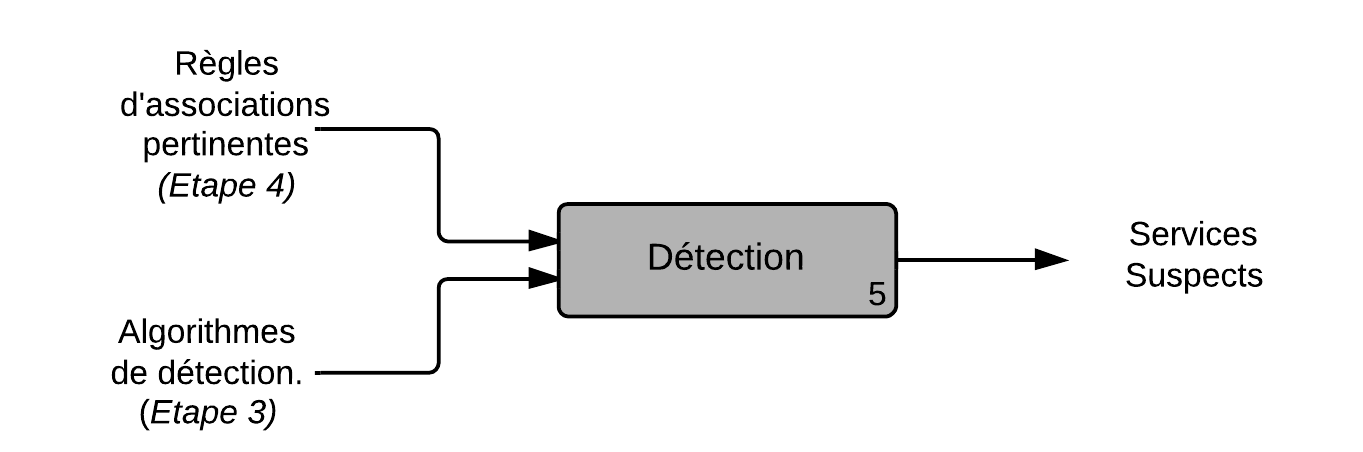
\includegraphics[scale=0.25]{media/step5.png}
\end{center}
\caption{\'Etape 5: D�tection d'anti-patrons SOA.\label{detec}}
\end{figure}

Le processus de d�tection est illustr� dans la figure \ref{TinyD}.
On s'aper�oit que toutes les r�gles d'association g�n�r�es depuis les traces d'ex�cution de la figure \ref{tinyR} impliquent une seule et m�me m�thode: \texttt{SA.mA}.
De plus, cette m�thode communique avec trois services distincts: B, C et D.
De ce fait, les resultats des m�triques NM (\textit{Number of Methods}) et OC (\textit{Outgoing Coupling}) seront respectivement 1 et 3.
Si ces valeurs sont jug�es statistiquement faibles et hautes sur l'�chelle de Likert respectivement, alors le service A sera identifi� comme un \textit{Tiny Service}, comme indiqu� dans la carte de r�gles pr�sent�e par la figure \ref{fig:rules}-b.

\begin{figure}
\begin{center}
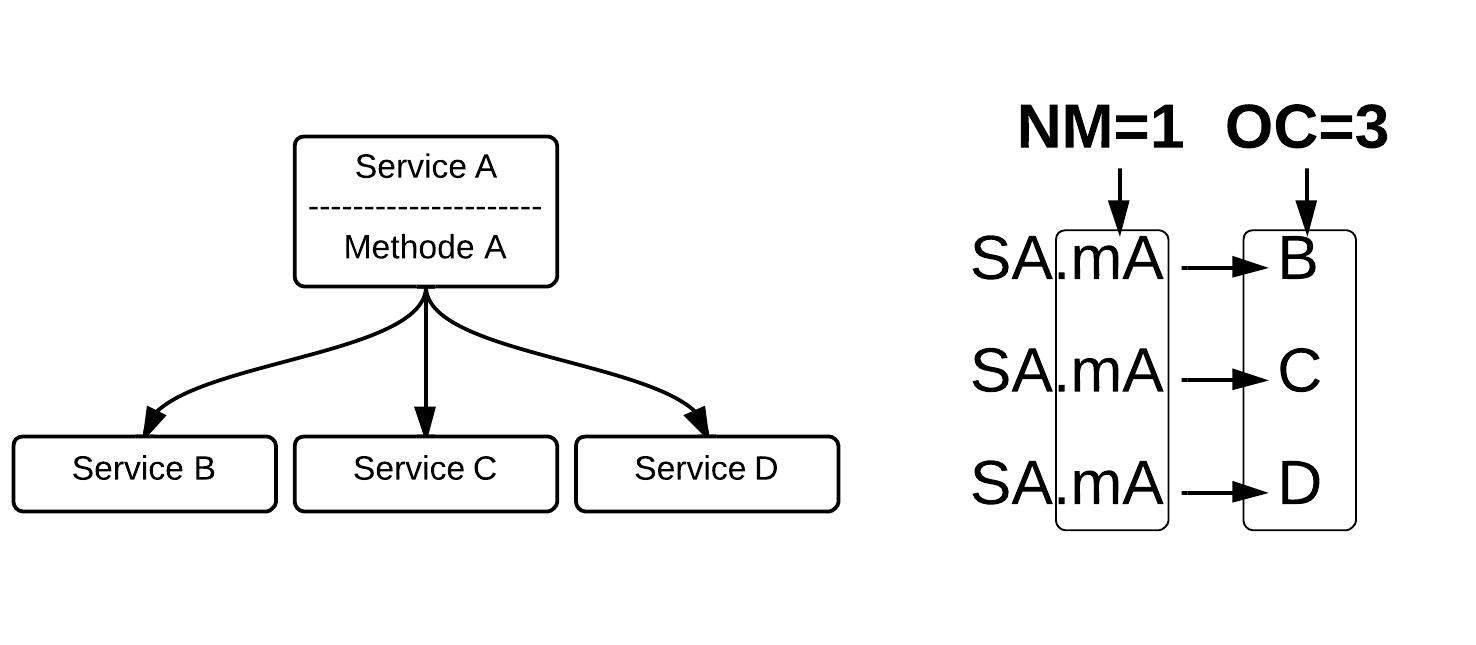
\includegraphics[scale=0.2]{media/Tiny-Detection.png}
\end{center}
\caption{D�tection d'un \textit{Tiny Service}.\label{TinyD}}
\end{figure}

Au cours de ce chapitre, nous avons pr�sent� en d�tail les cinq �tapes composant l'approche SOMAD pour la d�tection automatique d'antipatrons dans les applications � base de services.
Nous avons aussi pr�sent� les hypoth�ses, m�triques et processus de g�n�ration d'algorithme utilis�s pour cette d�tection.
Dans le prochain chapitre, nous pr�sentons l'impl�mentation qui supporte l'approche SOMAD.



\chapter{Impl�mentation de SOMAD}

Dans ce chapitre, nous pr�sentons l'impl�mentation qui supporte l'approche SOMAD.
Nous pr�sentons aussi les raisons techniques qui font en sorte que SOMAD a de meilleurs r�sultats que SODA, en termes de pr�cision et performances.
Nous allons tout d'abord �tudier la g�n�ration des traces d'ex�cution puis leur collecte et agr�gation.
Enfin, nous nous attarderons sur l'identification des transactions dans ces traces et la modification de l'algorithme RuleGrowth pour l'adapter � nos besoins.

\section{G�n�ration de traces d'ex�cution} 
Dans le cas o� les traces ne sont pas disponibles, cette �tape permet leur g�n�ration.
Si le syst�me � base de services cible ne produit pas de traces d'ex�cution qui contiennent toutes les informations requises, nous devons l'instrumentaliser dans ce but.
De telles traces permettent de d�boguer les applications quand des d�bogueurs ne sont pas disponibles ou applicables (souvent le cas dans les environnements SOA).
La production de traces d'ex�cution peut, cependant, introduire de l'obfuscation\footnote{Le code imp�n�trable ou offusqu� d'un programme informatique est un code dont la compr�hension est difficile pour un humain tout en restant parfaitement compilable par un ordinateur.} de code.
N�anmoins, elle peut aussi avoir des b�n�fices au niveau de la compr�hension de l'architecture car le code doit �tre parfaitement ma�tris� afin d'�tre instrumentalis� correctement.
Cette technique de production de traces d'ex�cution est la plus commune.
Cependant, si le code source n'est pas disponible, une autre technique consiste � instrumentaliser l'environnement d'ex�cution du syst�me � base de services cible.
Par exemple, LTTng \citep{Fournier2009} instrumentalise les syst�mes de type Linux afin qu'ils produisent des traces d'ex�cution avec un faible sur-co�t en termes de temps d'ex�cution.


Pour faciliter le traitement automatique des traces d'ex�cution, nous avons imagin� un mod�le (voir figure \ref{logs}) qui est un bon compromis entre simplicit� et quantit� d'informations.
Dans ce mod�le, une invocation de m�thode g�n�re deux lignes, une ligne d'ouverture et une ligne de fermeture avec l'identification d'un client correspondant � son @IP et un marqueur temporel (\textit{timestamp}).
La pr�sence de deux lignes est n�cessaire pour identifier des appels � d'autres services avant la fin de la m�thode.
En effet, les traces contiendront une nouvelle ligne d'entr�e dans une m�thode avant la ligne de fermeture de la m�thode initiatrice.

\begin{figure}[h]
\begin{center}
\framebox{\begin{minipage}[t]{10cm}%
IP timestamp void methodA.ServiceA();\\
~~~~IP~~~~timestamp void methodB.ServiceB();\\
~~~~IP~~~~timestamp end void methodB.ServiceB();\\
IP timestamp end void methodA.ServiceA();
\end{minipage}}
\caption{Mod�le de trace\label{logs}.}
\end{center}
\end{figure}

Les syst�mes � base de services contiennent souvent des sous-syst�mes de g�n�ration de traces d'ex�cution.
Cependant, ces syst�mes d�j� int�gr�s peuvent produire des traces tr�s diff�rentes de notre mod�le.
En cons�quence, nous avons rendu SOMAD adaptable par un simple DSL (\textit{Domain Specific Language}) bas� sur les expressions r�guli�res (voir figure \ref{dsl-}).
De ce fait, les informations peuvent �tre ordonn�es diff�remment.

\begin{figure}[h]
\begin{center}
\framebox{\begin{minipage}[t]{10cm}%
time\{\textasciicircum\textbackslash w+\textbackslash s\textbackslash d\textbackslash d\textbackslash s\textbackslash :\textbackslash d\textbackslash d:\textbackslash d\textbackslash d.\textbackslash d+\} end\{end\}\\
method\{\textasciicircum[\textasciicircum.]*.(.*)\$\}
service\{\$[\textasciicircum.]*.(*.)\}\\
customer\{\textbackslash b\textbackslash d\{1,3\}\textbackslash .\textbackslash d\{1,3\}\textbackslash .\textbackslash d\{1,3\}\textbackslash .\textbackslash d\{1, 3\}\textbackslash b\}\\
line\{ *customer *time *(end)? *method.service *\}
\end{minipage}}
\caption{DSL associ� au mod�le de la figure \ref{logs} \label{dsl-}.}
\end{center}
\end{figure}

\section{Collecte des traces d'ex�cution et agr�gation} Le but ici est de t�l�charger les fichiers de traces l� o� elles se trouvent puis de les agr�ger dans un seul et m�me fichier.

Les traces d'ex�cution sont g�n�r�es par les services composant le syst�me, puis elles sont collect�es et agr�g�es.
Cette �tape est importante -- elle construit les donn�es d'entr�e de SOMAD -- et non triviale \citep{Wilde2008}.
En effet, la nature hautement dynamique et distribu�e des syst�mes � base de services introduit deux d�fis distincts.
Le premier est li� � la distribution des syst�mes � base de services et, donc, des traces d'ex�cution.
En effet, chaque service g�n�re ses traces d'ex�cution dans son environnement propre.
De ce fait, nous devons conna�tre l'endroit o� s'ex�cutent les services et chaque environnement doit disposer d'un m�canisme pour t�l�charger les traces d'ex�cution.
Le second d�fi est li� au dynamisme; en effet, les services peuvent �tre consomm�s par de nombreux clients en m�me temps, et de ce fait, les traces d'ex�cution peuvent s'entrelacer.
Afin de r�soudre ces probl�mes, nous utilisons une approche bas�e sur celle de \citep{Yousefi2011} :

\begin{itemize}

\item Nous t�l�chargeons les traces d'ex�cution distribu�es dans l'architecture du syst�me � base de services en utilisant une base de connaissances pr�alable.
Cette base de connaissances contient les d�p�ts o� aller chercher les traces d'ex�cution, les protocoles, et toute autre information utile.

\item Nous rassemblons les diff�rents fichiers dans un fichier unique.

\item Nous trions les traces d'ex�cution en utilisant leurs marqueurs temps.
Cette �tape n�cessite que les diff�rents environnements d'ex�cution des diff�rents services soient synchronis�s sur la m�me horloge.
En r�gle g�n�rale, cette contrainte est facilement atteignable car les organisations peuvent se synchroniser avec des services d'horloge externe.

\item Nous exploitons les relations appelant-appel� entre services et m�thodes pour distinguer des blocs de transactions concurrentes.

\item Nous classons les transactions par client (IP).
\end{itemize}

\section{\green{Identification des transactions}}

Comme expos� dans les chapitres pr�c�dents, une transaction est une s�quence d'appels de services et de m�thodes.
Parmi les transactions identifi�es dans les traces d'ex�cution, nous nous focalisons uniquement sur les transactions contenant plus d'un service.
En effet, notre but �tant d'identifier des conceptions de faible qualit�, un appel unique ne peut que difficilement nous renseigner sur l'architecture sous-jacente.
\green{La figure \ref{traces} pr�sente des traces d'ex�cution indent�es\footnote{L'indentation ne fait pas partie du format. Elle a �t� introduite ici pour simplifier la lecture.} par transaction.} Une fois les transactions triviales --- contenant un appel --- retir�es de l'ensemble des transactions, deux tables de transactions --- et donc de r�gles d'association s�quentielles --- sont g�n�r�es.
La premi�re des deux tables est au niveau des services, tandis que la seconde est au niveau des m�thodes.
Ainsi, � chaque fois qu'une m�thode est invoqu�e, la premi�re table enregistre les services impliqu�s dans cet appel alors que la seconde enregistre les m�thodes impliqu�es.
G�n�rer deux tables � deux niveaux de granularit� diff�rent am�liore la performance de nos algorithmes.
En effet, la premi�re table � haute granularit� --- services --- est g�n�r�e en premier, et les algorithmes de d�tection sont appliqu�s � ce niveau.
Ensuite, l'investigation est pouss�e au second niveau de granularit� --- les services + les m�thodes --- uniquement pour les services d�sign�s comme suspects � la fin de la premi�re passe d'analyse.
Durant la premi�re phase, nous g�n�rons plus vite nos r�gles d'association s�quentielles car il y a moins d'objets, et durant la seconde, nous traitons moins de traces puisque les services non-suspects sont ignor�s.
Le cumul des deux traitements s'est r�v�l� plus performant qu'un traitement � granularit� fine -- m�thodes + services -- uniquement.

\begin{figure}
\framebox{\begin{minipage}[t]{\columnwidth}%
\begin{center}
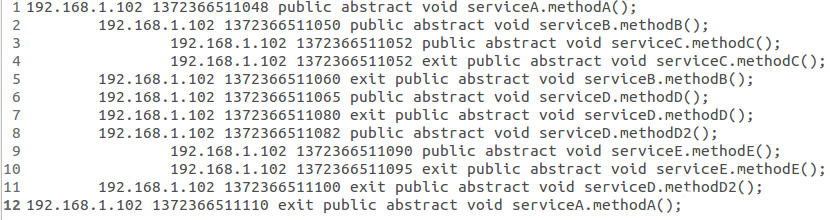
\includegraphics[scale=0.45]{media/traces.png}
\end{center}
\end{minipage}}
\caption{Traces d'ex�cution indent�es par transaction.\label{traces}}
\end{figure}

\begin{table}[h!]
\centering
\scriptsize
\begin{tabular}{|c|c|c|}
\hline
Transaction & Services participants & M�thodes participantes  \\
\hline
\hline
1 (Lignes 1 � 12) & (A, B, C, D, D, E) &  (A, B, C, D, D2, E) \\
2~~(Lignes 2 � 5) & (B, C) &  (B, C) \\
3 (Lignes 8 � 11) & (D, E) &  (D2, E) \\
\hline
\end{tabular}
\caption{Extraction d�sir�e.\label{tableTransaction}}
\end{table}

\green{Le tableau \ref{tableTransaction} pr�sente les transaction extraites par services et par m�thodes pour l'exemple de la figure \ref{traces}.
Nous y pr�sentons les deux tables de transactions.}

\green{Afin d'obtenir le r�sultat pr�sent� par le tableau \ref{tableTransaction}, nous avons con�u un algorithme d�di�.
Cet algorithme (Algorithme \ref{algoExtract}) a pour seul but de parcourir les traces d'ex�cution afin d'en extraire des s�quences qui seront par la suite utilisables par les algorithmes de fouille de r�gles d'association s�quentielles.
Cette algorithme vise l'extraction des diff�rentes transactions impliquant plus d'un service.}

L'intuition derri�re cet algorithme est plut�t simple.
En effet, pour chaque ligne dans les traces d'ex�cution, il d�termine si la ligne est un d�but ou une fin de transaction.
Si la ligne en cours est un d�but de transaction alors la position de l'algorithme dans les traces est sauvegard�e puis nous cherchons la fin de la transaction en cours.
Lorsque la fin est trouv�e, toutes les op�rations entre le d�but et la fin sont ajout�es � une nouvelle transaction.
Comme les transactions peuvent �tre imbriqu�es, l'algorithme retourne � la position qu'il avait sauvegard�e et cherche un nouveau d�but de transaction.
Ce processus est r�p�t� jusqu'� la fin des traces d'ex�cution.

Cet algorithme se compose de nombreuses boucles imbriqu�es.
La premi�re s'�tendant des lignes 2 � 20 permet simplement de d�rouler les traces d'ex�cution jusqu'� la fin.
A l'int�rieur de cette boucle, chaque trace $\kappa$ est analys�e (ligne 4) afin de d�terminer si c'est une trace de sortie (qui contient le mot clefs \texttt{exit}).
Si nous sommes en pr�sence d'une trace d'entr�e alors, cette trace est ajout�e � la transaction courante (ligne 6) et notre position dans l'ensemble des traces est sauvegard�e (ligne 5).
La prochaine op�ration consiste � trouver la fin de cette transaction.
Ceci est r�alis� par la boucle \texttt{tant que} s'�tendant des lignes 7 � 12.
A l'int�rieur de cette boucle, nous continuons � progresser dans l'ensemble des transactions et ajoutons les lignes ne contenant pas d'\texttt{end} � la transaction courante (ligne 10).
Nous progressons tant que la ligne courante ne correspond pas � la sortie de la transaction courante (ligne 7).
Lorsque les lignes $\kappa$ sont ajout�es � la transaction courante, en r�alit�, une ligne est ajout�e dans la transaction courante par service et une autre dans la transaction courante par m�thode.
La seule diff�rence entre ces lignes est leur formatage.
En effet, pour les m�thodes, la ligne est gard�e enti�re, tandis que pour les services, elle est tronqu�e pour ne conserver que le nom du service.
Finalement, si la transaction n'est pas triviale, c-�-d, qu'elle a une taille sup�rieure � 1 (sup�rieur � 1 service), nous l'ajoutons � l'ensemble des transactions (ligne 14).
Nous explorons ensuite la suite des transactions en repla�ant notre index � une ligne apr�s le d�but de la transaction que nous venons d'identifier � la ligne 16.


\begin{algorithm}[H]
\Indp
\Donnees{Traces d'ex�cution}
\Res{Transactions}
\BlankLine 
 \Pour{chaque ligne $\kappa$ dans les traces}{
  \eSi{$\kappa$ n'est pas une trace de sortie}{
  d�butDeTransaction $\leftarrow$ positionCourante\;
  $\kappa \leftarrow$ transactionCourante\;
  	\Tq{$\kappa_{positionCourante} \neq \kappa_{debutDeTransaction}$ }{positionCourante++\;
	\Si{$\kappa_{positionCourante}$ n'est pas une trace de sortie}{$\kappa_{positionCourante} \leftarrow$ transactionCourante\;}
  	} 
  	\Si{taille de transactionCourante $\neq$ 1}{transactionCourante  $\leftarrow$ Transactions\;}
  	positionCourante $\leftarrow$ d�butDeTransaction\;
   }{
   positionCourante++\;
  }
 }
 \caption{Extraction de transactions depuis des traces d'ex�cution format�es.\label{algoExtract}}
\end{algorithm}

\newpage

\section{\green{Adaptation de RuleGrowth pour la d�tection d'anti-patrons: SOARuleGrowth}}

L'algorithme RuleGrowth \citep{Fournier-viger2011} est un algorithme qui permet de fouiller des r�gles d'association s�quentielles dans de grand ensemble d'�v�nements qui peuvent �tre simultan�s.
Bien que performant en termes de temps d'ex�cution et de pr�cision, l'algorithme RuleGrowth n'est pas tout � fait adapt� � nos donn�es.
Dans les sous-sections suivantes, nous pr�sentons l'algorithme RuleGrowth et les am�liorations que nous lui avons apport�s afin qu'il soit mieux adapt� � nos donn�es et d'augmenter notre pr�cision.
 

\subsection{RuleGrowth}


L'algorithme \ref{RuleGrowth} expose les principes g�n�raux de l'algorithme de RuleGrowth.
Cet algorithme commence par diff�rencier les �l�ments fr�quents et les �l�ments non-fr�quents.
Ensuite, l'algorithme d�termine si deux �l�ments juxtapos�s poss�dent les valeurs n�cessaires, en termes de support et de confiance, pour la g�n�ration d'une r�gle.
Enfin, si une r�gle est g�n�r�e, elle peut �tre �tendue en y ajoutant de nouveaux candidats � droite ou � gauche.


Ces op�rations nomm�es \textit{Chercher de nouveaux �l�ments � gauche} et \textit{Chercher de nouveaux �l�ments � droite} sont des tentatives d'expansion de la r�gle d'association � gauche et � droite.
Dans les deux op�rations d'expansion, l'algorithme consid�re une r�gle ne poss�dant qu'un �l�ment de chaque cot� (A$\rightarrow$B) puis parcourt les �l�ments sur la gauche (droite) de l'�l�ment gauche (droit) des transactions dans lesquelles la r�gle (A$\rightarrow$B) appara�t.

Si la r�gle d'origine agr�ment�e d'un nouvel �l�ment � gauche (droite), est toujours sup�rieure aux minimums de confiance et de support requis, alors \textit{Chercher de nouveau �l�ments � gauche} (\textit{Chercher de nouveaux �l�ments � droite}) est rappel�e de mani�re r�cursive avec une r�gle de la forme KA$\rightarrow$B (A$\rightarrow$BK) afin de continuer l'expansion.


\green{Les �l�ments qui ne sont pas fr�quents --- qui n'apparaissent pas assez pour atteindre le seuil support fix� --- sont retir�s de l'ensemble des s�quences (ligne 1).
Ensuite, les �l�ments restants sont ajout�s � une liste d'�l�ments fr�quents lors d'une boucle s'�tendant des lignes 2 � 5.
\`A la fin de ces deux premi�res op�rations, nous avons une liste d'�l�ments sur lesquels travailler afin de g�n�rer des r�gles d'association s�quentielles.
Par la suite, nous trouvons une double boucle dans laquelle l'algorithme d�termine combien de partenaire communs ont deux �l�ments qui sont juxtapos�s (lignes 7 � 24).
Dans la seconde boucle --- celle qui est imbriqu�e --- si le nombre de partenaires identifi�s est sup�rieur au seuil, alors les r�gles sont g�n�r�es (IJ, ligne 15 et JI, ligne 20).
Finalement, l'algorithme tente d'�tendre la r�gle g�n�r�e en cherchant des �l�ments potentiels � droite et � gauche (lignes 16, 17, 21, 22).
}

\newpage

\begin{small}



%\linesnumbered
%\SetLine
\begin{algorithm}[H]
Retirer les �l�ments qui ne sont pas fr�quents\;

\Pour{tous les elements $\kappa$ restant dans Sequences}{
	\Si{Support de $\kappa$ $\succeq$ Support minimum}{
		$\kappa \leftarrow $ ElementsFrequents\;
	}
	}
	\Pour{tous les �l�ments $\kappa$I dans ElementsFrequents}{
		OccurrenceI  $\leftarrow$ compter nombre de $\kappa_I$\;
		PartenairesI  $\leftarrow$ Trouver partenaire dans OccurrenceI\;
		
			\Pour{tous les elements $\kappa$J dans 			ElementsFrequents � partir de position courante + 1}{
		OccurrenceJ $\leftarrow$ compter nombre de $\kappa$J\;
		PartenairesJ $\leftarrow$ Trouver partenaire dans OccurrenceJ\;
		
		Construire une liste de partenaires communs � I \& J\;
		
		\Si{le nombre de partenaires communs pour IJ est sup�rieur au support minimum}{
			G�n�rer la r�gle IJ\;
			Chercher de nouveaux �l�ments � gauche\;
			Chercher de nouveaux �l�ments � droite\;
		}
		
		\Si{le nombre de partenaires communs pour JI est sup�rieur au support minimum}{
			G�n�rer la r�gle JI\;
			Chercher de nouveaux �l�ments � droite\;
			Chercher de nouveaux �l�ments � gauche\;
		}
	}	
	}

 \caption{Algorithme RuleGrowth simplifi�\label{RuleGrowth}.}
\end{algorithm}

\end{small}

\subsection{Motivations et changements}

Malgr� les performances affich�es de \textit{RuleGrowth} et les excellents r�sultats que nous avons obtenus en l'utilisant --- 100\% rappel et une pr�cision sup�rieure � celle de SODA d'une marge allant de 2.6\% � 16.67\% --- cet algorithme poss�de des limitations --- li�es � nos donn�es --- qui doivent �tre combl�es afin d'extraire le maximum de connaissances des traces d'ex�cution.
Afin de combler ces limitations, nous avons effectu� trois changements majeurs sur l'algorithme originel d�crits ci-bas.

\begin{change}
\label{time} D�finir une fen�tre temporelle de travail
\end{change}

\green{\textit{RuleGrowth} ne poss�de pas de fen�tre temporelle d�finissable.
En effet, comme montr� par l'exemple d'introduction du Chapitre 2, les s�quences et leurs items ne sont pas horodat�s.
 De ce fait, si un utilisateur fait une pause significative dans son utilisation du SBS, les services invoqu�s avant cette pause pourront �tre associ�s avec les services invoqu�s apr�s cette pause et inversement.

Dans le but de ne pas biaiser les associations, il est imp�ratif de d�limiter une fen�tre temporelle dans laquelle diff�rents appels peuvent �tre associ�s.
Les s�quences accept�es devront donc avoir la forme suivante:  
\begin{center}
\texttt{timestamp\{a\}, timestamp\{b\}} 
\end{center}
o� \texttt{timestamp} sera remplac� par le temps Unix ou Posix.
Cette notation d�crit un instant dans le temps comme le nombre de seconde �coul�es depuis le 1 Janvier 1970 et \texttt{a} et \texttt{b} des items.
A titre d'exemple, \texttt{1386197722\{a\}} repr�sente l'invocation du service A le 5 d�cembre � 22H55 et 22 secondes.
\texttt{1386197723\{b\}} est l'invocation du service b une seconde plus tard.

Afin d'obtenir le comportement d�sir�, nous avons modifi� la seconde boucle \texttt{Pour} de l'algorithme \ref{RuleGrowth} par une boucle \texttt{Tant que} qui s'ach�ve lorsqu'il n'y a plus d'�l�ments � parcourir ou lorsque la fen�tre temporelle s�parant deux �l�ments devient sup�rieure � celle indiqu�e par l'utilisateur.
N�anmoins, comme pr�sent� � la figure \ref{timewindows}, il faut faire la diff�rence entre des traces qui sont temporellement distantes les unes des autres � cause d'une pause dans l'utilisation et celles qui sont distantes dans le temps � cause du temps d'ex�cution d'une m�thode.
Le cas particulier d'un arr�t impr�vu du syst�me en cours de transaction (\textit{crash}) est g�r� par l'algorithme d'extraction de transaction \ref{algoExtract}.
De la m�me mani�re, les fonctions \textit{Chercher de nouveaux �l�ments � gauche} et \textit{Chercher de nouveaux �l�ments � droite} pr�sentes dans l'algorithme \ref{RuleGrowth} aux lignes 16, 17 et 21, 22, respectivement, ont �t� modifi�es pour prendre en compte la fen�tre temporelle.}

\begin{figure}
\begin{center}
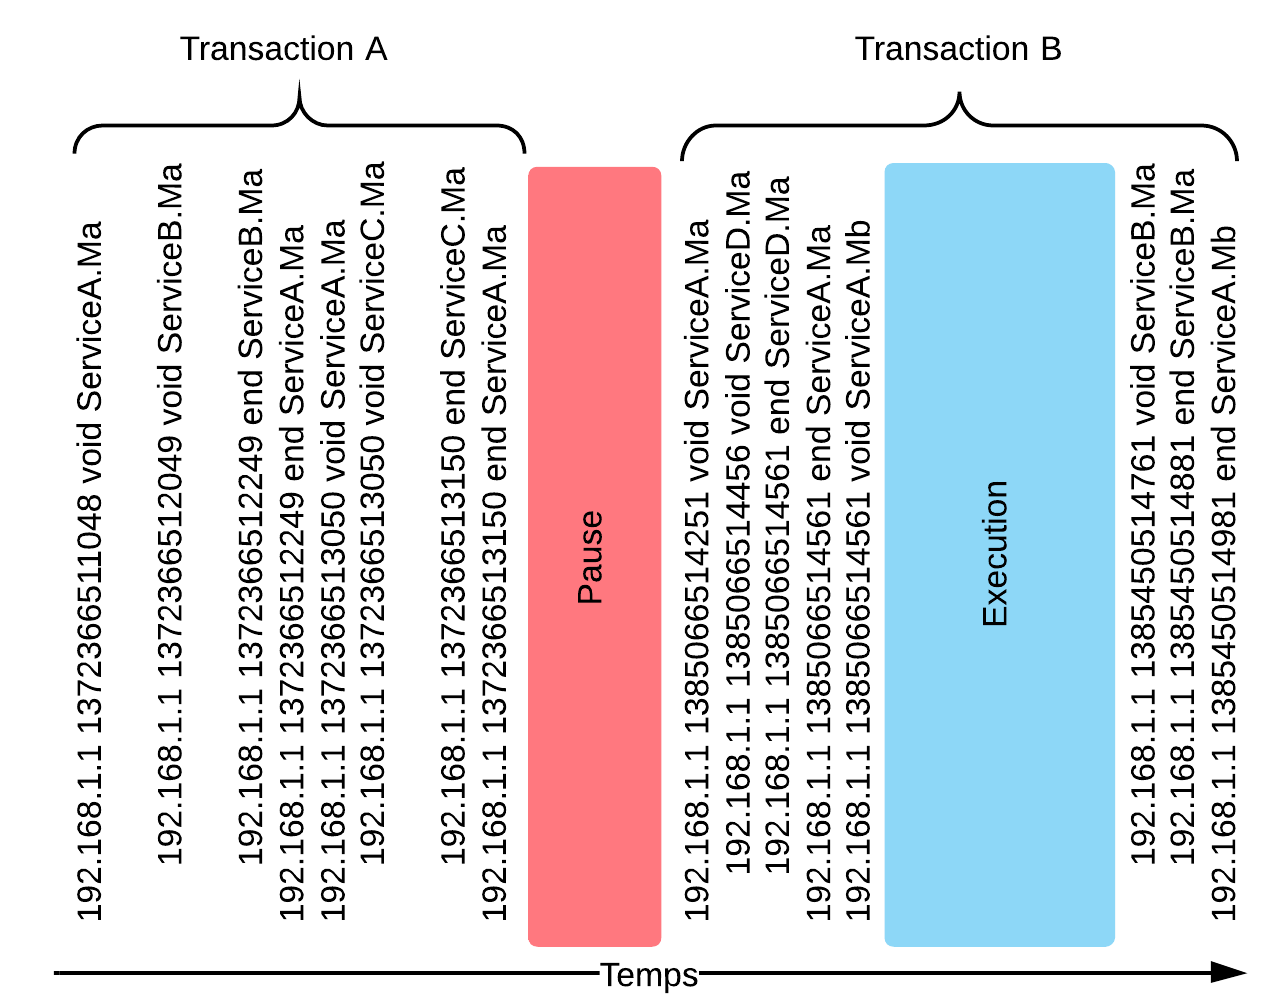
\includegraphics[scale=0.25]{media/timeWindows.png}
\end{center}
\caption{Exemple de fen\^etres de temps\label{timewindows}.}
\end{figure}

\begin{small}

\end{small}

%\linesnumbered
%\SetLine
\begin{algorithm}
	\Pour{tout $\kappa_I$ $\in$ $Elements_{Frequents}$}{
		Occurrence$_I$  $\leftarrow$ compter nombre de $\kappa_I$\;
		Partenaires$_I$  $\leftarrow$ Trouver partenaire dans Occurrence$_I$\;
		$\kappa_J$  $\leftarrow$ $Elements_{Frequents}$ � la position $\kappa_I$ + 1\;
			\Tq{ $\kappa_J$ $\neq$ $\emptyset$ \& (MarqueurTemps$_{\kappa_J}$ - MarqueurTemps$_{\kappa_I} \leq $ Fen�tre$_{max}$)}{
					OccurrenceI  $\leftarrow$ compter nombre de $\kappa$I\;
		PartenairesI  $\leftarrow$ Trouver partenaire dans OccurrenceI\;
		
			\Pour{tout $\kappa$J $\in$ $Elements_{Frequents}$ � partir de $position_{courante}$+1}{
		Occurrence$_J$  $\leftarrow$ compter nombre de $\kappa$J\;
		Partenaires$_J$  $\leftarrow$ Trouver partenaire dans OccurrenceJ\;
		
		Construire une liste de partenaires communs � I \& J\;
		
		\Si{le nombre de partenaires communs pour IJ est  $>$ � $supp_{min}$}{
			G�n�rer la r�gle IJ\;
			Chercher de nouveaux �l�ments � gauche et � droite\;
		}
		
		\Si{le nombre de partenaires communs pour JI $>$ � $supp_{min}$}{
			G�n�rer la r�gle JI\;
			Chercher de nouveaux �l�ments � gauche et � droite\;
		}
	}	
			
			$\kappa_J$  $\leftarrow$ ElementsFrequents a la position $\kappa_{J + 1}$\;
	}
	
}
 \caption{Modifications relatives au changement \ref{time}.\label{timealgo}}
\end{algorithm}

\begin{change}
\label{threads}
Regrouper des appels quasi-simultan�s
\end{change}

\green{Les transactions extraites par l'algorithme \ref{algoExtract} sont uniquement compos�es d'�l�ments --- invocations --- simples.
Du point de vue de RuleGrowth, cela signifie que les invocations ne sont pas simultan�es.
Bien que n'�tant pas exactement simultan�s, il peut �tre pertinent de regrouper des �v�nements \textit{presque} simultan�s en un unique �l�ment.
Gr�ce � ce regroupement nous pourrons, par exemple, identifier des m�thodes dont la premi�re action est d'en appeler une autre et augmenter le poids de la relation (couplage) entre ces m�thodes.}


\begin{figure}[h!]
\begin{center}
\framebox{\begin{minipage}[t]{10cm}%
IP timestamp void methodA.ServiceA();\\
~~~~IP~~~~timestamp void methodB.ServiceB();\\
~~~~IP~~~~timestamp end void methodB.ServiceB();\\
//~~~~Traiement de la m�thode A \\
//~~~~Invocation des m�thodes C, D et E entrecoup�es de traitements.\\
IP timestamp end void methodA.ServiceA();
\end{minipage}}
\end{center}
\caption{Appels quasi-simultan�s.}
\end{figure}

\green{ dispose d'une extraction identique �: \texttt{(A,B)(C)(D)\~(E)} plut�t que \texttt{(A)(B)(C)(D) (E)}.
De cette mani�re nous renfor�ons la relation entre A et B.
Une phase de pr�traitement doit �tre ajout�e afin que si \texttt{timestamp\{a\}, timestamp\{b\}} poss�dent un \texttt{timestamp} �gal ou tr�s proche, alors la s�quence soit transform�e en \texttt{timestamp\{a, b\}}.
Cet ensemble sera d�sormais consid�r� comme une suite de deux �v�nements simultan�s.
L'algorithme \ref{threadsalgo} pr�sente le pr�traitement n�cessaire sur les donn�es avant de lancer l'algorithme \textit{SOARuleGrowth}.
De la m�me mani�re que pr�sent� pr�c�demment par l'algorithme \ref{timealgo}, nous avons mis en place une boucle \texttt{Tant Que} qui prend fin lorsqu'il n'y a plus d'�l�ment ou lorsque la fen�tre temporelle relative au rassemblement d'�v�nements est d�pass�e (lignes 5 � 7).
N�anmoins, � l'int�rieur de cette boucle, les �l�ments satisfaisant les conditions sont ajout�s � une liste d'�l�ments nomm�e composition (ligne 6), puis les �l�ments ajout�s sont supprim�s de la liste principale d'�l�ments (ligne 8).
Si la composition ainsi cr��e dispose d'�l�ments (ligne 10), alors nous rajoutons l'�l�ment duquel nous �tions parti � la t�te de la composition et le supprimons de la liste principale (ligne 11 et 12).
Enfin, nous ajoutons la composition nouvellement cr��e � la liste principale � la position courante (ligne 13).}


%\linesnumbered
%\SetLine
\begin{algorithm}
	\Pour{tous les �l�ments}{
		$\kappa_J$ $\leftarrow$ �l�ment � la position $\kappa_I$ + 1\;
			\Tq{ $\kappa_J$ $\neq$ $\emptyset$ \& (MarqueurTemps$_{\kappa_J}$ - MarqueurTemps$_{\kappa_I} \leq $ Fen�tre$_{max}$)}{
			$\kappa_J$ $\leftarrow$ composition\;
			Supprimer $\kappa$J dans �l�ments\;
			$\kappa_J$ $\leftarrow$ �l�ment � la position $\kappa$J + 1\;
	}
	
	\Si{Taille de la composition\ $\succ$ 0}{
		Placer $\kappa_I$ � la t�te de la composition\;
		Supprimer $\kappa_I$ dans �l�ments\;
		composition $\leftarrow$ �l�ments � la position $\kappa_I$\;
	}
	
}
 \caption{Modifications relatives au changement \ref{threads}.\label{threadsalgo}}
\end{algorithm}

\newpage

\begin{change}
\label{chain}
\'Eliminer les appels redondants
\end{change}

\green{Lors de nos tests pr�liminaires o� nous avons utilis� la version originale de \textit{RuleGrowth}, une proportion significative de faux positifs provenaient des appels de services � leurs propres m�thodes.
Ainsi, si un \texttt{ServiceA} invoque sa propre m�thode B au cours de l'invocation --- par un client externe ou un autre service --- de sa m�thode A, alors des r�gles de type : \texttt{ServiceA.methodA $\rightarrow$ ServiceA.methodB} pouvaient �tre g�n�r�es et fausser les m�triques de couplage et de d�pendance.
En effet, l'algorithme ne doit pas consid�rer comme pertinent les sous-s�quences de type : \texttt{\{ServiceA.methodA, ServiceA.methodB, ServiceA.methodC\}} car elles augmentent artificiellement le couplage du service en introduisant A comme partenaire de lui-m�me.
Afin d'introduire ce comportement sp�cifique dans l'algorithme \textit{RuleGrowth}, nous avons imagin� l'algorithme \ref{chainalgo}.
A chaque fois qu'une r�gle est sauvegard�e, nous v�rifions si deux �l�ments juxtapos�s dans cette r�gle appartiennent au m�me service (ligne 3).
Si tel est le cas, le second �l�ment est supprim� de la r�gle (ligne 4).}


%\linesnumbered
%\SetLine
\begin{algorithm}
	\Pour{tous les �l�ments d'une r�gle d'association}{
	
	\Si{	($\kappa_J$ $\leftarrow$ $\kappa_I$ + 1)  $\neq$ $\emptyset$}{
	
		\Si{Service$_{\kappa_J}$ est egal � Service$_{\kappa_I}$}{
			Supprimer $\kappa_J$ de la r�gle d'association\;
			Calculer le support et la confiance de la r�gles sans  $\kappa_J$\;
			\Si{Support ou Confiance inf�rieurs aux seuils fix�s}{
				Supprimer la r�gle\;
			}
		}
	
	}
}
 \caption{Modifications relatives au changement \ref{chain}.\label{chainalgo}}
\end{algorithm}

\green{\subsection{Impacts des modifications}}

\green{Afin de mesurer l'impact de ces modifications, nous avons compar� les deux algorithmes en termes de nombres de r�gles g�n�r�es, de longueur moyenne des r�gles, le temps et de la m�moire n�cessaire � leur g�n�ration.
Nous avons test� les algorithmes en utilisant les donn�es utilis�es pour nos exp�rimentations du prochain chapitre.
Le figure \ref{nb-rules} expose le nombre de r�gles � des supports fix�s (60\%, 40\%, 20\% et 10\%).
Le nombre de r�gles g�n�r�es par \textit{SOARuleGrowth} est inf�rieur de 36\% pour un support �gal � 10\%.
Cette diff�rence significative est due aux changements interdisant de sauvegarder une r�gle compos�e d'�l�ments r�partis avant et apr�s une pause ainsi qu'au regroupement d'appels presque simultan�s --- r�duisant le nombre d'�l�ments, et donc, le nombre de possibilit�s pour cr�er des r�gles.}

\begin{figure}
\begin{center}
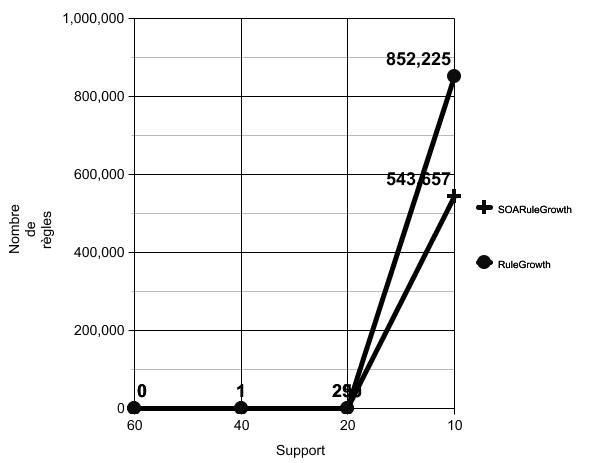
\includegraphics[scale=0.6]{media/graph.jpg}
\end{center}
\caption{Nombre de r�gles\label{nb-rules}.}
\end{figure}

\green{Notre seconde mesure concerne la longueur moyenne des r�gles g�n�r�es.
Le graphe \ref{taille-rules} expose les diff�rences entre \textit{SOARuleGrowth} et \textit{RuleGrowth}.
Le changement~\ref{chain} sp�cifie l'�limination des r�gles qui augmentaient artificiellement le couplage d'un service.
De plus, un patron \texttt{$ServiceA.methodA \Rightarrow Service.A.methodB$} sera aussi �limin�.
En cons�quence, la longueur moyenne des r�gles d'association diminue l�g�rement.}

\begin{figure}
\begin{center}
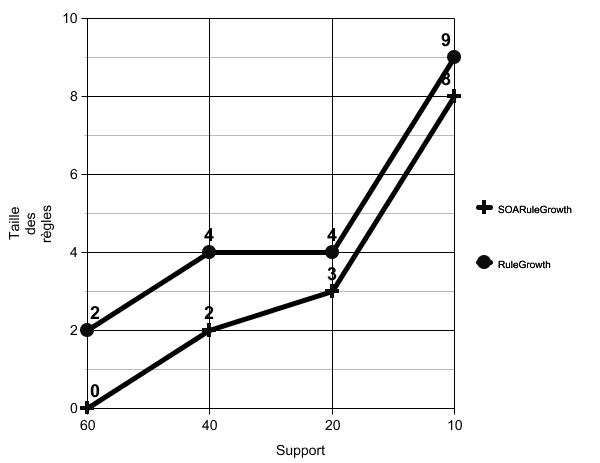
\includegraphics[scale=0.6]{media/graph(1).jpg}
\end{center}
\caption{Longueur moyenne des r�gles d'association\label{taille-rules}.}
\end{figure}

\green{Le graphique \ref{mo-rules} pr�sente l'impact de nos modifications en termes de m�moire n�cessaire.
On constate que \textit{SOARuleGrowth} est moins gourmand que son pr�d�cesseur lorsque le support minimum � atteindre est haut car il traite moins d'�l�ments et donc moins d'�l�ments fr�quents et de r�gles d'association.
Cependant, la sup�riorit� s'inverse pour un support � 10\%.
Ceci est principalement est li� au fait que (1) les �l�ments trait�s par SOARuleGrowth sont plus gros, ils contiennent l'horodatage et (2) le temps requis pour le pr�-traitement n�c�ssaire � \textit{SAORuleGrowth} est directement li� au nombre d'�l�ments � traiter. 
Avec un support si faible, un nombre tr�s cons�quent d'�l�ments est trait�, et donc la diff�rence entre les algorithmes se fait ressentir.}

\begin{figure}
\begin{center}
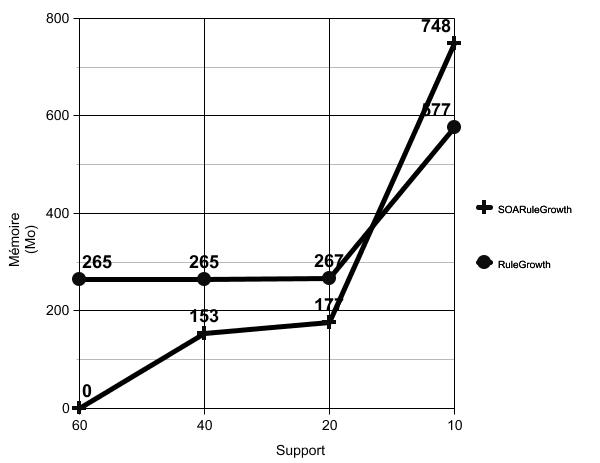
\includegraphics[scale=0.6]{media/graph(2).jpg}
\end{center}
\caption{M�moire requise\label{mo-rules}.}
\end{figure}

\green{La derni�re mesure que nous avons effectu�e est pr�sent�e par la figure \ref{time-rules}.
Cette derni�re mesure le temps d'ex�cution des deux algorithmes.
La diff�rence n'est pas significative; en effet, au maximum, \textit{SOARuleGrowth} est plus lent que son pr�d�cesseur de 7.8\%.
Cette diff�rence s'explique � cause du pr�-traitement suppl�mentaire requis par \textit{SOARuleGrowth} par rapport � \textit{RuleGrowth}.}

\begin{figure}
\begin{center}
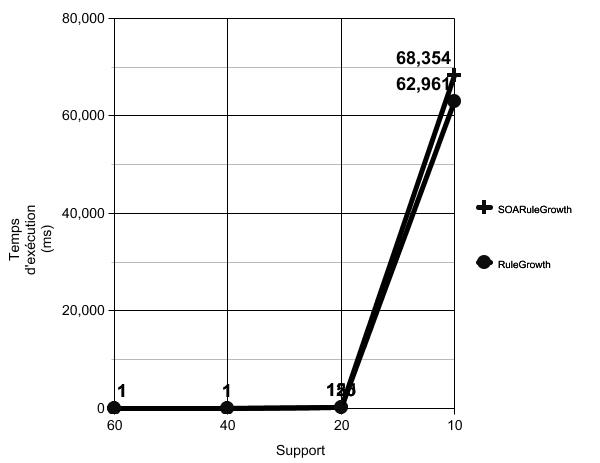
\includegraphics[scale=0.6]{media/graph(3).jpg}
\end{center}
\caption{Temps d'ex�cution\label{time-rules}.}
\end{figure}

\section{Changement d'objectif} Cette section explique pourquoi SOMAD obtient de meilleurs r�sultats que SODA pour identifier des anti-patrons qui sont plus � m�me d'endommager la qualit� de service d'un SBS.
En effet, la pr�sence d'un anti-patron dans une partie peu visit�e du syst�me fait courir des risques plus faibles aux cr�ateurs du syst�me.

Les hypoth�ses de SOMAD changent l'objectif de la recherche d'anti-patrons SOA d'une consid�ration de conception pure vers une consid�ration d'utilisation.
C'est � dire que nous cherchons � identifier les anti-patrons qui sont provoqu�s par la mani�re dont les utilisateurs consomment les services que le SBS offrent plut�t que par les collaborations statiques entre les services.
 De ce fait, SOMAD n�glige les valeurs de m�triques basiques.
 C'est un choix naturel, car SOMAD est une approche qui n'a pas acc�s aux valeurs exactes au travers des interfaces des services ou leurs impl�mentations.
De plus, analyser un syst�me � base de services via son utilisation plut�t que son architecture, comme l'indiquent les r�sultats exp�rimentaux d�crits dans le chapitre \ref{exp}, entra�ne une pr�cision bien sup�rieure.
Consid�rons un service nomm�e \texttt{Half-Deprecated Service} (figure \ref{Hds}) compos� de quatre m�thodes: A, B, C and D.
Les m�thodes C et D sont d�pr�ci�es\footnote{La d�pr�ciation est, dans le domaine du d�veloppement logiciel, la situation o� une ancienne fonctionnalit� est consid�r�e comme obsol�te au regard d'un nouveau standard, bien qu'elle soit conserv�e dans les versions plus r�centes pour des fins de compatibilit�.} mais sont tout de m�me expos�es pour assurer la r�tro-comptabilit� de ce service avec ces clients.


\begin{figure}
\begin{center}
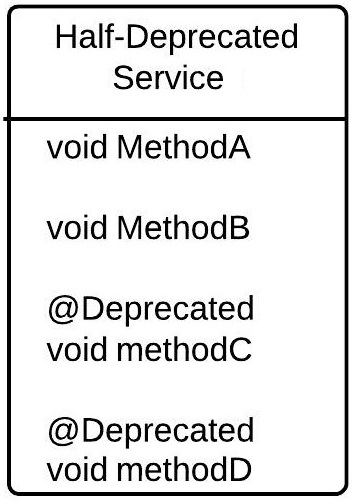
\includegraphics[scale=0.30]{media/half.jpeg}
\end{center}
\caption{Repr�sentation pseudo-UML du \texttt{Half-Deprecated Service}.\label{Hds}}
\end{figure}

Une m�thode pour calculer la coh�sion d'un service est de compter combien de m�thodes du service sont utilis�es durant une session unique d'un utilisateur unique.
Comme la moiti� des m�thodes sont d�pr�ci�es, il est fort probable que le client ne consomme que la moiti� des m�thodes.

\begin{itemize}
\item Soit le client est un ancien client et il utilisera les deux m�thodes d�pr�ci�es.
\item Soit le client est un nouveau client et il utilisera les deux m�thodes non d�pr�ci�es.
\end{itemize}

De ce fait, si la coh�sion est calcul�e de cette mani�re, le r�sultat sera 0.5 (2/4) et ce service sera consid�r� comme suspect pour les anti-patrons SOA qui sont identifiables par une faible coh�sion.
Au contraire, si la coh�sion est calcul�e en utilisant une m�thode bas�e sur les traces d'ex�cution, le r�sultat aura plus de chance d'�tre pr�s de 1.
En effet, les appels aux m�thodes d�pr�ci�es ne devraient pas appara�tre dans les r�gles d'association s�quentielles, car ils ne devraient pas atteindre le seuil minimum de confiance et de support.

\section{Conclusion}

Dans ce chapitre, nous avons pr�sent� l'impl�mentation qui supporte l'approche SOMAD ainsi qu'une am�lioration de \textit{RuleGrowth} nomm�e \textit{SOARuleGrowth} et des consid�rations sur le changement d'objectif dans la d�tection  d'anti-patrons.
Toutes ces modifications ont fait progresser notre pr�cision de 3\% par rapport � l'algorithme classique. De plus, le temps d'ex�cution de \textsc{SOMAD} (\textit{SOARuleGrowth} + calcul des m�triques et r�gles) est directement impact� par:
\begin{itemize}
\item \emph{La taille des traces d'ex�cution}. En effet, plus le nombre de traces augmente, plus les algorithmes de pr�-traitement et de g�n�ration de r�gles d'association vont avoir besoin de temps.
\item \emph{La complexit� de connexion inter-services} (profondeur maximale des transactions). Ceci est d� au fait que le temps n�cessaire au d�coupage des traces d'ex�cution en transaction est impact� par la profondeur de la pile. 
\item \emph{Le nombre de m�triques � calculer}. Une fois les r�gles d'association calcul�es il faut calculer les m�triques des tableaux \ref{MetricsS} et \ref{MetriquesC} afin de d�tecter les anti-patrons. 
\item \emph{La complexit� des r�gles de d�tection des anti-patrons} (nombres d'intersections, exclusions,...).
\item \emph{Le nombre de services}. En effet, les m�triques doivent �tre calcul�es pour chaque service; ainsi le nombre de services est un facteur important.
\end{itemize}


Dans le prochain chapitre, nous aurons un aper�u de la r�action de \textit{SOARuleGrowth} face � la mise � l'�chelle (\textit{scalability}). En effet, nous avons men� nos exp�riences sur deux syst�mes diff�rents qui ont la particularit� d'�tre compos�s de 13 et 130 services. Les traces d'ex�cutions produites par ces syst�mes, quant � elles, passent de $\sim$1500 � $\sim$10 000 lignes. Malgr� l'augmentation de la taille du syst�me (x10) et celle des traces (x6.6), le temps d'ex�cution moyen par anti-patron n'est multipli� que par $\sim$4 passant de 0.068s � 0.280s. Nous pouvons donc dire que SOMAD supporte bien la mise � l'�chelle; d'autant plus qu'un syst�me � base de services compos� de 130 services peut �tre consid�r� comme un syst�me de taille industrielle. Le chapitre \ref{exp} pr�sentera aussi la validation empirique de notre approche et de nos algorithmes.


\chapter{Exp�rimentations et validation}
\label{exp}
Afin de valider notre approche, nous avons appliqu� SOMAD sur deux syst�mes � base de services d�velopp�s ind�pendamment, \textit{HomeAutomation} et \textit{FraSCAti} \citep{Seinturier2012}.
\textit{HomeAutomation} est compos� de 13 services tandis que FraSCAti est 10 fois plus important: 91 composants et 130 services.
Nous avons choisi d'exp�rimenter notre approche sur ces syst�mes car ce sont ceux qui ont permis de valider SODA --- l'approche pr�liminaire --- et nous allons de ce fait, pouvoir comparer les deux approches en termes de pr�cision et de rappel d'un cot�, et d'efficacit� de l'autre.

Dans ce chapitre nous pr�senterons les hypoth�ses qui nous ont servi � valider nos exp�rimentations, puis nous pr�senterons en d�tail nos sujets d'exp�rimentation.
Enfin, nous pr�senterons notre mode op�ratoire ainsi que nos r�sultats.

\section{Hypoth�ses}

Les exp�rimentations visent � valider les trois hypoth�ses suivantes:

\begin{hypothesis}
\textbf{Pr�cision.} Les algorithmes de d�tection doivent avoir un rappel de 100\%, c'est-\`a-dire, que tous les anti-patrons pr�sents sont d�tect�s, et une pr�cision sup�rieure � 75\%, c'est-\`a-dire, que parmi les anti-patrons d�tect�s, plus des trois-quarts sont de vrais positifs.
\end{hypothesis}

Cette premi�re hypoth�se supporte l'exactitude des r�gles d'association s�quentielles g�n�r�es ainsi que leur interpr�tation via nos m�triques.
De plus, cette hypoth�se est similaire � celle qui ont permis de valider SODA car nous souhaitons que SOMAD soit, au minimum, aussi pr�cis que SODA.

\begin{hypothesis}
\textbf{Performance.} Le temps d'ex�cution requis par les algorithmes de d�tection sont aussi bas que ceux de SODA, c'est-\`a-dire, en dessous d'une seconde.

\end{hypothesis}

Cette deuxi�me hypoth�se supporte la performance de SOMAD par rapport � SODA en termes de temps d'ex�cution. 
Ce choix d'une seconde est une approximation grossi�re de ce qui peut �tre consid�r� comme non-intrusif en termes de temps d'attente pour un utilisateur souhaitant am�liorer la qualit� de son syst�me � base de services via la d�tection d'anti-patrons. 
Dans un futur proche, nous souhaiterions pouvoir int�grer la d�tection d'anti-patrons pendant le d�veloppement des applications en analysant les traces produites � chaque compilation \& lancement. 
De ce fait, 1 seconde nous para�t �tre acceptable.

\begin{hypothesis}
\textbf{Extensibilit�.} SOMAD est extensible dans le sens o� on peut lui ajouter de nouveaux anti-patrons et les d�tecter.
\end{hypothesis}

Avec cette derni�re hypoth�se � valider par nos exp�rimentations, nous voulons montrer combien il est ais� d'ajouter ou de combiner des m�triques afin de d�tecter de nouveaux anti-patrons.

\section{Sujets}
Nous avons appliqu� SOMAD pour d�tecter six anti-patrons SOA d�crits dans le tableau \ref{tab:List-of-SOA}.
Dans la description de chaque anti-patron, nous avons mis en gras les caract�ristiques importantes pour leurs d�tections via nos m�triques des tableaux~\ref{MetricsS} et \ref{MetriquesC}.

\section{Objets}
Une premi�re passe d'exp�rimentation a �t� r�alis�e sur \textit{HomeAutomation}.
\textit{HomeAutomation} est une application de type SCA d�velopp�e ind�pendamment pour le contr�le domotique de maisons de personnes �g�es (temp�rature, instruments �lectriques, urgences m�dicales).
Cette application inclut 7 sc�narios pr�d�finis � des fins de tests et de d�monstration.
Deux versions diff�rentes du syst�me ont �t� utilis�es: la version originale avec 13 services et une version d�grad�e intentionnellement dans laquelle des services ont �t� modifi�s et d'autres ajout�s afin d'injecter de  nouveaux anti-patrons SOA.
Ces changements ont �t� r�alis�s par une tierce partie afin d'�viter de biaiser les r�sultats.
La figure \ref{fig:HA} pr�sente l'architecture d'\textit{HomeAutomation} tandis que la figure \ref{fig:HMA} pr�sente son interface graphique.

\begin{figure*}

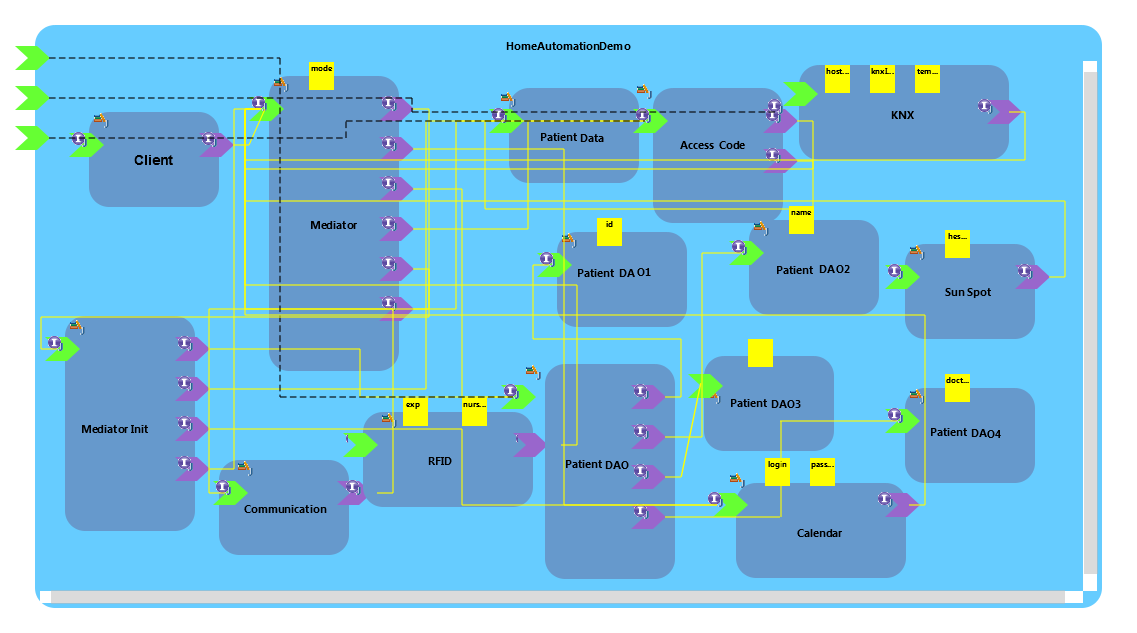
\includegraphics[scale=0.35]{media/Home-Automation.png}%

\caption{\label{fig:HA}Diagramme SCA d'\textit{HomeAutomation}.}
\end{figure*}

\begin{figure*}
\begin{center}
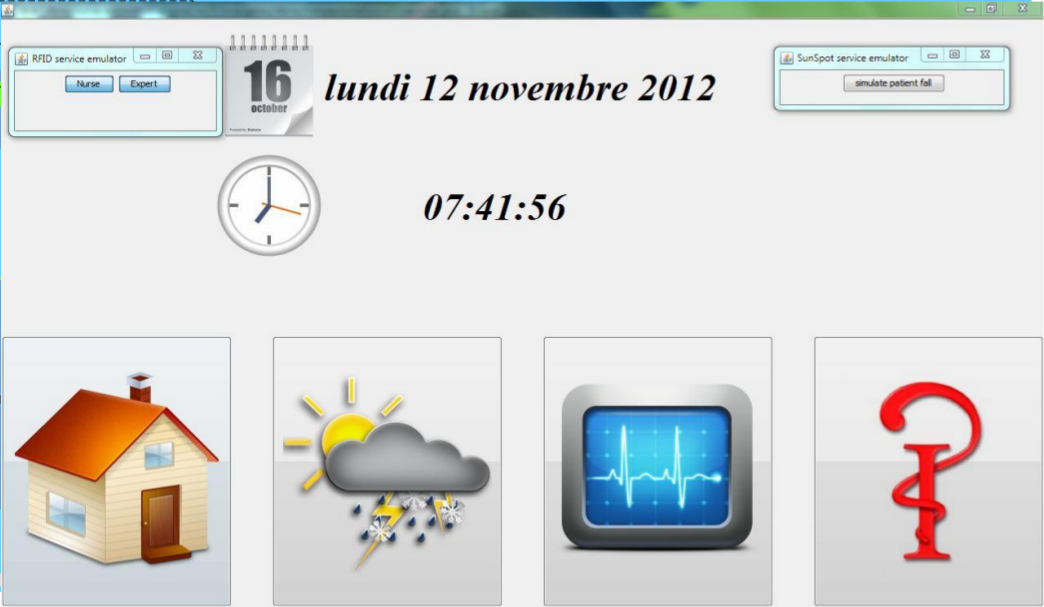
\includegraphics[scale=0.35]{media/HMA.png}%
\end{center}
\caption{\label{fig:HMA}Interface graphique d'\textit{HomeAutomation}.}
\end{figure*}

\'Etant donn� le manque de syst�mes � base de services disponibles gratuitement, la seconde passe d'exp�rimentation a �t� r�alis�e sur le support d'ex�cution d'\textit{Home\-Automation}: \textit{FraSCAti} \citep{Seinturier2012}.
\textit{FraSCAti} est aussi un syst�me de type SCA compos� de 91 composants et 130 services.
Les services sont distribu�s dans les composants et un composant expose au moins un service.
Contrairement � \textit{HomeAutomation}, \textit{FraSCAti} ne poss�de pas de sc�narios pr�d�finis --- en r�alit�, il comporte quelques tests unitaires, mais pas de couverture compl�te des fonctionnalit�s.
La d�tection a �t� effectu�e en instrumentalisant \textit{FraSCAti} afin qu'il produise des traces d'ex�cution tel que d�crit dans le chapitre pr�cedent.
Comme \textit{FraSCAti} est un environnement d'ex�cution pour les syst�mes SOA, nous avons charg� et lanc� des syst�mes de diverses technologies (SCA, REST, Web-Service, RMI) dans \textit{FraSCAti}; puis nous avons utilis� ces syst�mes dans le but de couvrir un maximum de fonctionnalit�s de \textit{FraSCAti}.


La figure \ref{fig:FRA} pr�sente l'architecture de FraSCAti tandis que la figure \ref{fig:FSCRIPT} pr�sente l'interface graphique de l'explorateur de service.

\begin{figure*}

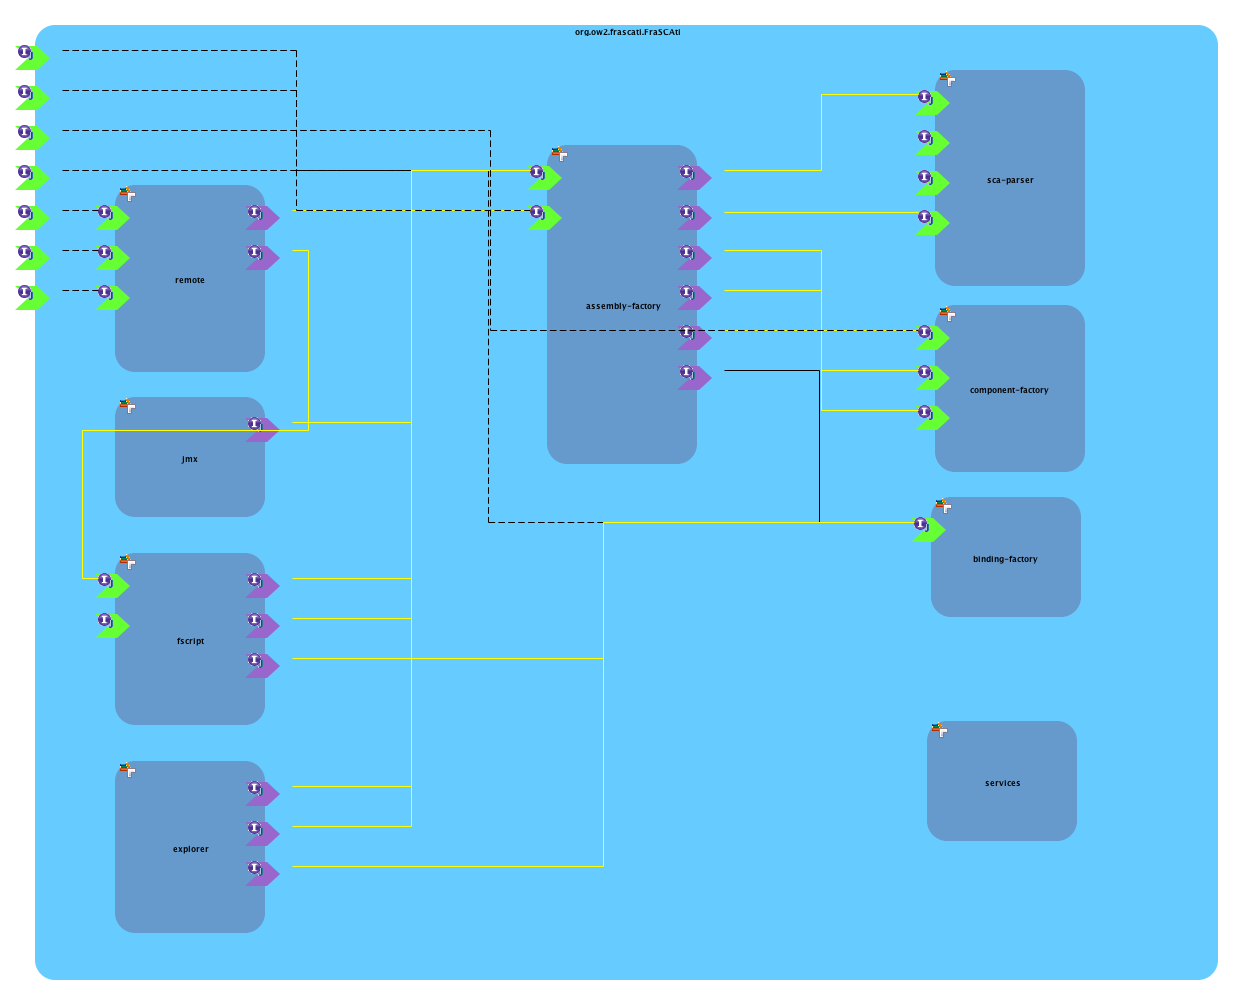
\includegraphics[scale=0.45]{media/FraSCAti.png}%

\caption{\label{fig:FRA}Diagramme SCA principal de \textit{FraSCAti}.}
\end{figure*}

\begin{figure*}
\begin{center}
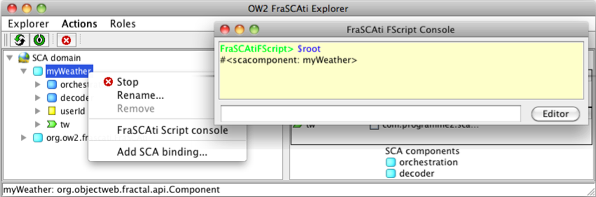
\includegraphics[scale=0.45]{media/fscript-console.png}%
\end{center}
\caption{\label{fig:FSCRIPT}Interface graphique de l'explorer \textit{FraSCAti}.}
\end{figure*}

La d�tection d'anti-patrons SOA sur \textit{FraSCAti} a �t� effectu�e au niveau des composants plut�t qu'� celui des services � cause de sa documentation.
En effet, \textit{FraSCAti} est document� au niveau des composants et c'est cette documentation qui sera utilis�e pour la validation des r�sultats.
De plus, nous avons empiriquement prouv� que les syst�mes SCA souffrent des m�mes maux architecturaux que les syst�mes SOA purs.


D'autres d�tails sur les syst�mes analys�s peuvent �tre trouv�s en ligne: 

\begin{itemize}
\item \url{http://sofa.uqam.ca/somad}
\item \url{http://frascati.ow2.org/doc/1.4/ch12s04.html}
\end{itemize}

Le tableau \ref{Objects: Two Versions of Home-Automation} pr�sente un comparatif entre \textit{HomeAutomation} et \textit{FraSCAti} en termes de taille, nombre de services, nombre de m�thodes et nombre de classes.

\begin{table}[h!]
\centering
\scriptsize
\begin{tabular}{|l|c|c|c|c|c|}
\hline
Application & Version & Taille & NDS & NDM & NDC \\
\hline
\hline
Home Automation & original & 3.2 MLDC & 13 & 226 & 48 \\
Home Automation & d�grad�e & 3.4 MLDC & 16 & 243 & 52 \\
FraSCAti & original & 26.75 MLDC & 130 & 1882 & 403 \\
\hline
\end{tabular}
\caption{Propri�t�s d' \textit{Home-Automation} et \textit{FraSCAti} (NDS: Nombre De Services, NDM: Nombre de M�thodes, NDC: Nombre de classe, MLDC: Milliers de lignes de code).}
\scriptsize{\label{Objects: Two Versions of Home-Automation} }
\end{table}

\section{\green{Mat�riel et langage}}

Les exp�rimentations ont �t� men�es sur un poste avec les caract�ristiques suivantes:

\begin{itemize}
\item Ubuntu Release 12.04 (precise) 64-bit
\item Kernel Linux 3.5.0-36-generic
\item M�moire vive: 5.8 GB
\item Processeur : 2x Intel Xeon(R) CPU E5345 @ 2.33GHz x 4
\end{itemize}

Le langage de programmation choisi pour l'impl�mentation de SOMAD est Java :

\begin{itemize}
\item Version: 1.6.0\_27.
\item Machine Virtuelle: OpenJDK 64-Bit Server VM (build 20.0-b12, mixed mode).
\end{itemize}



\section{\green{L'outil \textsc{Somad}}}

\green{Nous avons d�velopp� l'outil \textsc{Somad} en ad�quation avec l'approche du m�me nom.
\textsc{Somad} a quatre fonctionnalit�s principales:}

\begin{itemize}
\item La sp�cification d'anti-patrons SOA en utilisant les m�triques de notre catalogue
\item La d�tection automatique d'antipatrons dans les SOAs
\item La visualisation du syst�me cible
\end{itemize}

\green{La figure \ref{guiSomad} pr�sente l'interface graphique de \textsc{Somad}.
On y constate une visualisation des services pr�sents sous forme de noeuds ainsi que les communications entre les services sous forme d'ar�tes.
Les services (noeuds) color�s en rouge signifient que le service est impliqu� dans un anti-patron.
L'outil affiche aussi la pile d'appel sur le panneau de gauche.}

\begin{figure}
\begin{center}
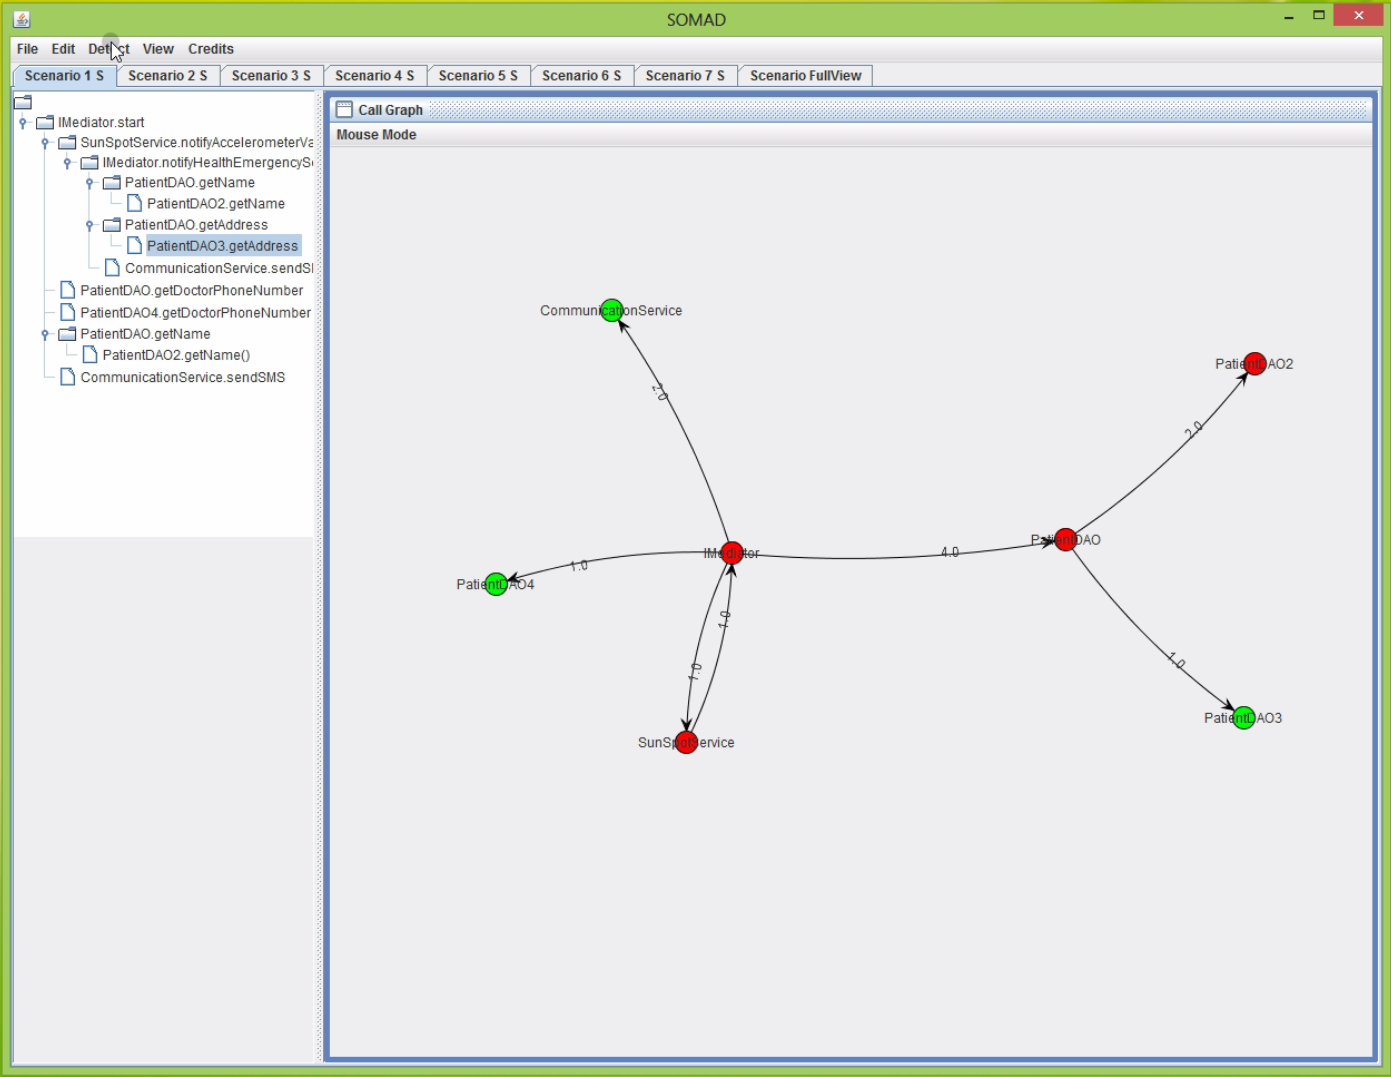
\includegraphics[scale=0.39]{media/GUI-SOMAD.png}
\caption{Interface de l'outil \textsc{Somad}.\label{guiSomad}}
\end{center}
\end{figure}

\green{De plus une autre fonctionnalit� prometteuse est actuellement en cours de d�veloppement.
Cette fonctionnalit� consiste � ajouter de nouveaux services en utilisant leur d�finition (comme, par exemple, un WSDL), puis nous recalculons la d�tection des anti-patrons SOA en consid�rant ces ajouts.
Une vid�o de l'outil \textsc{Somad} (en anglais) est disponible sur notre site institutionnel: \url{http://sofa.uqam.ca/somad/}.}

\section{\green{Processus}}



Nous avons appliqu� SOMAD pour la d�tection de six anti-patrons SOA sur deux syst�mes distincts.
Tout d'abord, nous avons lanc� les sept sc�narios d'\textit{Home\-Automation}:

\begin{itemize}
\item D�tection de la chute d'un patient et envoi d'un message d'urgence au m�decin contenant l'adresse du patient (Services impliqu�s: \texttt{SunSpot Service}, \texttt{Communication Service}, \texttt{Mediator}).

\item Identique au sc�nario 1 mais planifie aussi un rendez-vous entre le patient et le m�decin � une date ult�rieure (Services impliqu�s: \texttt{SunSpot Service}, \texttt{Communication Service},\texttt{ Calendar Service}, \texttt{Mediator}).

\item Ajout d'un rendez-vous dans l'agenda du docteur (Services impliqu�s: \texttt{Communication Service}, \texttt{Calendar Service}, \texttt{Mediator}).

\item Contr�le des fen�tres et transfert de la responsabilit� du patient � une infirmi�re ou un technicien (Services impliqu�s: \texttt{RFID Service}, \texttt{Mediator}).

\item Contr�le des lumi�res dans la maison (Services impliqu�s: \texttt{RFID Service}, \texttt{Mediator}, \texttt{Communication Service}).

\item Contr�le des lumi�res et des fen�tres (Services impliqu�s: \texttt{KNX Service}, \texttt{Mediator}).

\end{itemize}

Ensuite, nous avons charg�, lanc� et utilis� cinq syst�mes diff�rents dans \textit{FraSCAti}:

\begin{itemize}
\item Une calculatrice bas�e sur des services web.
\item Un chat utilisant le Java RMI\footnote{\textit{Remote Method Invocation}, plus connu sous l'acronyme RMI est une interface de programmation (API) pour le langage Java qui permet d'appeler des m�thodes distantes}.
\item Une impl�mentation de la suite de Fibonacci bas�e sur des services REST
\item Une application de vente utilisant trois composants SCA dont un �crit en BPEL\footnote{En informatique, Business Process Execution Language, est un langage de programmation destin� � l'ex�cution des processus d'affaires.}
\item Une application de m�t�o consommant des services web distants
\end{itemize}

Une fois les traces g�n�r�es, nous les avons r�unies au sein d'un fichier distinct par application et extrait les transactions.
Sur ces transactions, nous avons appliqu� les algorithmes de fouille de r�gles d'association s�quentielles avec un support minimum de 40\% et une confiance minimum de 60\%.
 Ces choix ne suivent pas d'indications sp�cifiques li�es � l'ARM (\textit{Association Rule Mining}) ou intuitions particuli�res sur nos sujets d'exp�rimentations.
 En effet, nous �tions seulement guid�s par le besoin de filtrer toutes les r�gles non pertinentes tout en gardant assez de r�gles pour repr�senter la majorit� des appels.
De plus, nous avions besoin d'un minimum de confiance �lev�e pour faire appara�tre les alternatives les plus probables (cons�quent) pour chaque conclusion de transaction (ant�c�dent) tout en supprimant les moins significatives.
De ce fait, nous avons r�alis� plusieurs essais pour les deux seuils et observ� la taille de l'ensemble de r�gles.
\green{Afin de d�terminer quels �taient les meilleurs seuils, nous avons r�alis� des essais incr�mentaux en partant de 10\% et 40\%, respectivement pour le support et la confiance.
Pour chaque essai, nous avons augment� la valeur d'une des variables de 5\% et observ� la taille du r�sultat.
Les valeurs actuelles semblent apporter le meilleur compromis entre la taille de l'ensemble de r�gles et la pertinence des r�gles.
} 

L'�tape suivante consiste en l'interpr�tation des r�gles d'association s�quentielles g�n�r�es.
Dans ce but, nous avons appliqu� nos m�triques qui correspondent aux hypoth�ses bas�es sur les descriptions textuelles  des anti-patrons.
Enfin, nous avons valid� les r�sultats en termes de pr�cision et de rappel en analysant manuellement les syst�mes.
La pr�cision (Equation \ref{precision}) estime le ratio de vrais positifs dans les services suspects.
Le rappel (Equation \ref{recall}), quant � lui, estime le ratio d'anti-patrons d�tect�s sur le total d'anti-patrons pr�sents dans l'application.

\begin{equation}\label{precision}
\textit{pr�cision} = \frac{|\{\textit{anti-patrons}\;\textit{existants}\} \cap \{\textit{anti-patrons}\;\textit{d�tect�s}\}|}{|\{\textit{anti-patrons}\;\textit{d�tect�s}\}|}
\end{equation}

\begin{equation}\label{recall}
\textit{rappel} = \frac{|\{\textit{anti-patrons}\;\textit{existants}\} \cap \{\textit{anti-patrons}\;\textit{d�tect�s}\}|}{|\{\textit{anti-patrons}\;\textit{existants}\}|}
\end{equation}

Nous avons aussi �valu� nos performances gr�ce � la mesure $F_{1}$ (Equation \ref{measure}), qui est une moyenne pond�r�e de la pr�cision et du rappel pour mesurer l'exactitude de nos algorithmes de d�tection.

\begin{equation}\label{measure}
\textit{Mesure F$_{1}$} = 2 \times \frac{\textit{pr�cision} \times \textit{rappel}}{\textit{pr�cision} + \textit{rappel}}
\end{equation}

Cette validation a �t� r�alis�e manuellement par deux ing�nieurs logiciels ind�pendants, � qui nous avons fourni les descriptions des anti-patrons, les deux versions d'\textit{HomeAutomation} et le d�tail des composants de \textit{FraSCAti}.
Pour les deux syst�mes, les r�sultats ont �t� compar�s � ceux de SODA.
Pour \textit{FraSCAti}, nous avons rapport� notre d�tection � l'�quipe en charge de son d�veloppement et obtenu une validation objective de leur part.


\section{R�sultats}

Le tableau \ref{tab:Results-comparison-between} pr�sente les r�sultats de la d�tection des six anti-patrons SOA sur \textit{HomeAutomation}.
Pour chaque anti-patron, le tableau contient les services d�tect�s  automatiquement par SOMAD, les services identifi�s manuellement, les valeurs des m�triques, le rappel et la pr�cision, le temps de d�tection, et finalement  la mesure $F_{1}$.
De la m�me mani�re, le tableau \ref{tab:Results-comparison-between-1} rapporte les r�sultats de la d�tection sur \textit{FraSCAti}.
Nous rappelons que les valeurs des m�triques ne refl�tent pas les valeurs r�elles des services (par exemple, le nombre de m�thodes), mais une repr�sentation de la fa�on dont le syst�me est utilis� (via les traces d'ex�cution).
De plus, les valeurs des m�triques sont pond�r�es par la fraction $\frac{support}{confiance}$ dans le but d'accentuer le poids des r�gles d'association s�quentielles qui disposent de la plus grande confiance.
De ce fait, un nombre de m�thodes �gal � 2 veut dire que parmi les r�gles d'association s�quentielles g�n�r�es, il y a 2 m�thodes qui appara\^issent dans des r�gles disposant d'un fort support et d'une forte confiance.

\green{Le temps requis moyen est de 174ms pour SOMAD et de 469ms pour SODA.
Ceci est d� principalement au fait que SODA utilise la programmation orient�e aspects (AOP, Aspect Oriented Programming) pour attacher le code des m�triques sur chaque m�thode de chaque service d�couvert.
De plus, les m�triques sont attach�es une par une, par cons�quent, l'ex�cution du SOA sous analyse est interrompue autant de fois qu'il y a de m�triques � calculer, et ce � chaque invocation de m�thodes.
Au contraire, SOMAD n'interrompt pas l'application et n'est pas bas� sur l'AOP, ainsi il offre de bien meilleures performances.}

\begin{table*}
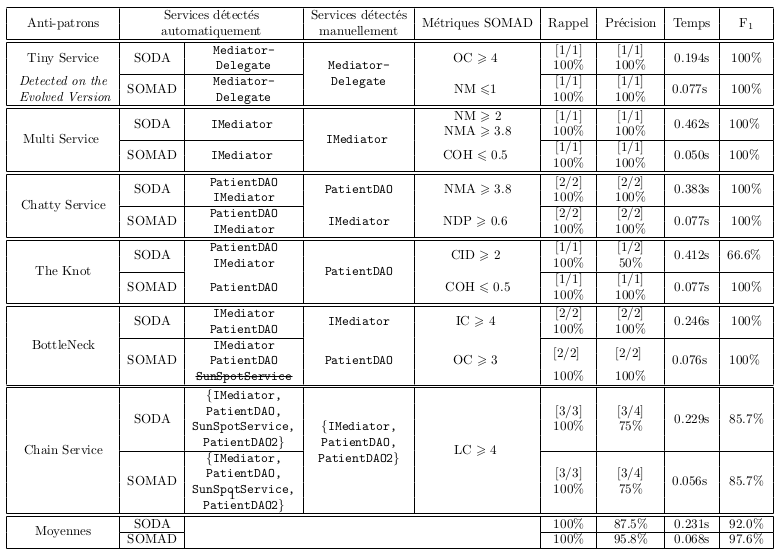
\includegraphics[scale=0.51]{media/HomeAutomationResults.png}%
 \caption{Comparaison des r�sultats de SOMAD et SODA sur \textit{HomeAutomation}\label{tab:Results-comparison-between}. Les services barr�s indiquent des faux-positifs d�tect�s par \textit{RuleGrowth} et pas par \textit{SOARuleGrowth}.}
\end{table*}


\begin{table*}
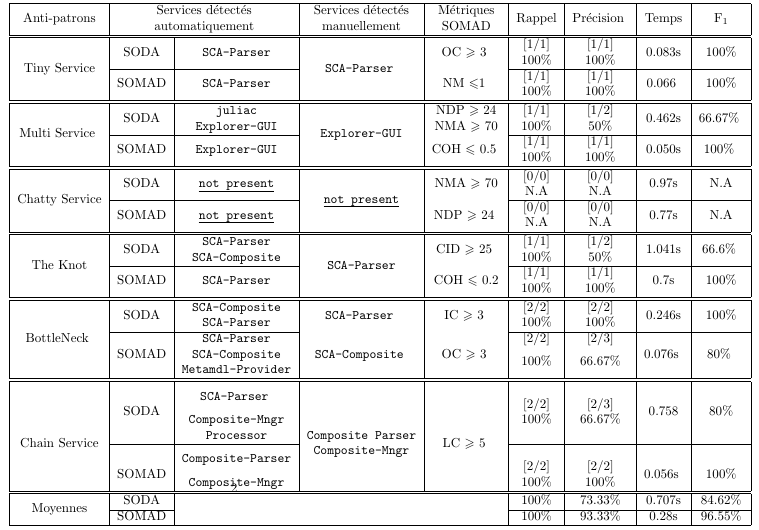
\includegraphics[scale=0.51]{media/FraSCAtiResults.png}%
\caption{Comparaison des r�sultats de SOMAD et SODA sur \textit{FraSCAti}.\label{tab:Results-comparison-between-1}}
\end{table*}

\section{D�tails des r�sultats}

Nous pr�sentons les r�sultats de d�tection de SOMAD tout en les comparants � SODA, sur \textit{HomeAutomation} et \textit{FraSCAti}.
Les r�sultats sont similaires, mis � part pour le \textit{Knot} et le \textit{BottleNeck}.


\subsection{\textit{HomeAutomation}}

\texttt{IMediator} a �t� d�tect� et identifi� comme un \textit{Multi Service} par SODA et SOMAD, � cause de son grand nombre de m�thodes (\textit{\textbf{N}umber of \textbf{M}ethods} $\geq$ 2), son grand nombre d'apparitions dans les r�gles (\textit{\textbf{N}umber of \textbf{MA}tches} $\geq$ 3.8) et sa faible coh�sion (\textit{\textbf{COH}} $\leq$ 0.5).
Les valeurs de ces m�triques on �t� �valu�es hautes et faibles en comparaison avec les scores obtenus par les autres services d'\textit{HomeAutomation}.
En effet, la technique de la boite � moustache (Boxplot en anglais) estime qu'un score $\geq$ 2 pour la m�trique \textbf{NM} est fort dans la distribution statistique des valeurs obtenues par les autres services.
De la m�me mani�re, les services d�tect�s comme \textit{Tiny Service} ont un petit nombre de m�thodes (\textbf{NM} $\leq$ 2) et un fort couplage sortant (\textit{\textbf{O}utgoing \textbf{C}oupling} $\geq$ 4), � nouveau en accord avec la boite � moustache.
Dans la version originale d'\textit{HomeAutmation}, nous n'avons pas d�tect� de \textit{Tiny Service}.
Dans le but d'�prouver nos algorithmes de detection, un ing�nieur ind�pendant a injecter cet anti-patrons.
En effet, il a extrait une m�thode du service \texttt{IMediator} et l'a d�plac�e dans un service nomm� \texttt{MediatorDelegate}; ce nouveau service a �t� d�tect� comme \textit{Tiny Service}.
Deux occurrences  du \textit{Chatty Service} ont �t� d�couvertes dans \textit{HomeAutomation} par SODA et SOMAD.
\texttt{PatienDAO} et \texttt{IMediator} apparaissent un grand nombre de fois dans les r�gles (\textbf{NMA} $\geq$ 3.8) --- ce qui signifie qu'ils communiquent avec beaucoup d'autres services --- et ils ont un grand nombre de partenaires diff�rents (\textbf{N}umber of \textbf{D}ifferent \textbf{P}artners $\geq$ 0.6).

\texttt{PatientDAO} a �t� d�tect� comme un \textit{Knot} car il une forte d�pendance cyclique d'invocation (\textit{\textbf{C}ross \textbf{I}nvocation \textbf{D}ependencies} $\geq$ 2).
Dans \textit{HomeAutomation}, un ensemble de services \texttt{PatientDAO1}, \texttt{PatientDAO2}, \texttt{PatientDAO3} et \texttt{PatientDAO4} sont fortement coupl�s car chacun d'entre eux repr�sente une partie des informations d'un patient (nom, adresse, num�ro de t�l�phone, num�ro de t�l�phone du docteur).
De ce fait, des invocations cycliques syst�matiques entre ces services apparaissent quand le syst�me souhaite acc�der aux informations compl�tes du patient.
SOMAD n'a pas d�tect� le faux positif \texttt{IMediator} d�tect� par SODA, et de ce fait, obtient une meilleure pr�cision pour cet anti-patron.

Deux services ont �t� d�tect�s comme �tant des \textit{BottleNeck}: \texttt{IMediator} et \texttt{Patient\-DAO} � cause de leur fort couplage entrant (\textbf{OC} $\geq$ 3) et sortant (\textit{\textbf{I}ncoming \- \textbf{C}oupling}~$\geq$~4).


Finalement, SODA et SOMAD ont d�tect� une cha�ne  d'invocations transitives ou \textit{Service Chain}: \texttt{IMediator} $\rightarrow$ \texttt{PatientDAO} $\rightarrow$ \texttt{PatientDAO2} $\rightarrow$ \texttt{SunSpotService} (\textbf{TC} $\geq$ 4).
Les deux approches rapportent le faux positif \texttt{SunSpotService}.

\subsection{\textit{FraSCAti}}

Nous pr�sentons maintenant les r�sultats des d�tections effectu�es sur \textit{FraSCAti}.

\texttt{SCA-Parser} est suspect� d'�tre un \textit{Tiny Service} car il a un faible nombre de m�thodes (\textbf{NM} $\leq$ 1) et un fort couplage sortant (\textbf{OC} $\geq$ 3).
Une inspection manuelle du code de \textit{FraSCAti} a r�v�l� que le service \texttt{SCA-Parser} ne contient qu'une seule m�thode nomm�e \texttt{parse}.
L'�quipe de d�veloppement de \textit{FraSCAti} a valid� cette d�tection.
Ils ont indiqu� que ce service peut �tre utilis� seul uniquement quand la lecture d'un fichier SCA est demand�e.
Cependant, \textit{FraSCAti} permet d'effectuer un grand nombre de t�ches qui auront besoin  de \texttt{SCA-Parser}.
Ces autres t�ches sont d�l�gu�es � d'autres services tels que \texttt{AssemblyFactory}.
Ceci explique le fort couplage sortant.
 

SOMAD n'a pas d�tect� de \textit{Multi Service} dans \textit{FraSCAti}.
Cependant, l'inspection manuelle a r�v�l� que le composant \texttt{Explorer-GUI} en est une occurence.
L'�quipe de d�veloppement de \textit{FraSCAti} a valid� que ce composant utilise un grand nombre d'autres services fournis par d'autres composants.
En effet, ce composant encapsule l'interface graphique de l'explorateur \textit{FraSCAti} qui fournit une interface exhaustive de toutes les fonctionnalit�s offertes par \textit{FraSCAti}.
SOMAD n'a pas �t� capable de le d�tecter car le processus d'exp�rimentation n'implique, � aucun moment, l'interface graphique.

SOMAD n'a pas d�tect� de \textit{Chatty Service}.
En effet, aucun service ne dispose de nombreuses apparitions dans les r�gles (\textbf{NMA}) et d'un grand nombre de partenaires diff�rents (\textbf{NDP}), respectivement sup�rieurs � 70 et 24 qui repr�sentent les seuils minimaux pour �tre consid�r� comme haut par la boite � moustache.
Cela signifie qu'aucun service n'apparait plus de 70 fois dans les r�gles et ne communique avec plus de 24 autres services.
L'inspection manuelle de \textit{FraSCAti} n'a pas permis d'identifier un tel anti-patron.
Nous avons exclus les r�sultats pour le \textit{chatty service} du calcul des moyennes. En effet, nous savons que SOMAD ne d�tecte pas de faux positifs sur cet anti-patron, mais nous ne pouvons pas �tre s�r que SOMAD d�tecterai un vrai positif s'il en rencontrai un dans \textit{FraSCAti}.

Le composant \texttt{Metamodel-Provider} est suspect� de faire partie d'un \textit{Knot} car il a une faible coh�sion (\textbf{COH} $\leq$ 0.2) et un nombre important de d�pendances cycliques (\textbf{CID} $\geq$ 25).
La validation par l'�quipe de d�veloppement de \textit{FraSCAti} confirme que ce composant est au centre de large flux de communications multidirectionnelles, mais ils ne sont pas d'accord sur la sp�cification de cet anti-patron particulier.

SOMAD a aussi d�tect� trois occurrences de \textit{BottleNeck}: \texttt{SCA-Parser}, \texttt{Composite\-Parser} et \texttt{Metamodel-provider}.
Toutefois, le dernier des trois est un faux positif.
Ces services ont �t� identifi�s comme \textit{BottleNeck} car ils disposent d'un fort couplage sortant et entrant, tous deux sup�rieur ou �gal � 3.


Finalement, le \texttt{Composite-Parser} (\textbf{TC} $\geq$ 4) a �t� d�tect� et identifi� comme partie d'un \textit{Service Chain}, tandis que le \texttt{Composite\~-Manager} est un faux positif.
L'�quipe de d�veloppement de \textit{FraSCAti} a confirm� que le \texttt{Composite-Parser} utilisait une cha�ne de d�l�gation pour compl�ter son abstraction.


Nous pouvons observer que le \texttt{Composite-Parser} et \texttt{SCA-Parser} sont des services suspects.
Ces services sont tr�s coupl�s avec d'autres services et, en particulier, ils font partie de longues cha�nes d'invocations.
La pr�sence de tels anti-patrons dans ce syst�me s'explique car il n'existe pas de mani�re de d�velopper de parseur sans introduire un fort couplage et une forte transitivit�.

En conclusion, \textit{FraSCAti} obtient de bons r�sultats quant � la d�tection d'anti-patrons.
Peu de services ont �t� d�tect�s comme tels en comparaison du grand nombre de services/composants pr�sents dans le syst�me.

\subsection{\green{Etude des faux positifs}}

\green{Nous �tudions maintenant les raisons qui ont men�s � la d�tection de faux positifs dans \textit{HomeAutomation} et \textit{FraSCAti}}.

\subsubsection{\green{\textbf{HomeAutomation}}}

\green{Le seul faux positif dans \textit{HomeAutomation} concerne le \texttt{SunSpotService} en tant que \textit{Chain Service}.
�tant donn� que SODA d�tecte aussi ce faux positif, et apr�s v�rification des analyses manuelles, il semblerait que \texttt{SunSpotService} ne soit pas un faux positif, mais une erreur apport�e par l'analyse manuelle.}


\subsubsection{\green{\textbf{FraSCAti}}}

\green{Le seul faux positif d�tect� par SOMAD sur \textit{FraSCAti} est le \texttt{Metamodel-Provider} en tant que \textit{BottleNeck}.
Une caract�ristique non n�gligeable pour identifier un \textit{BottlNeck} est son fort temps de r�ponse d� au fait qu'il est un goulot d'�tranglement dans le syst�me.
N�anmoins, nous avons d�ploy� tous les services de \textit{FraSCAti} en local lors de nos exp�rimentations et n'avions donc aucune information pertinente � tirer des temps de r�ponses des services --- compris entre 0.1s et 0.5s.
Afin d'augmenter notre pr�cision sur cet anti-patron, nous devrions consid�rer l'ajout d'une nouvelle m�trique \textbf{RT} (\textit{Repsonse Time}) qui mesurerait le temps de r�ponse des services en utilisant les marqueurs temps des traces d'ex�cution.
Cependant, cette m�trique s'appliquerait directement sur les traces, et non sur les r�gles d'association, ce qui pose un probl�me de compatibilit� d'informations.
En effet, nous ne pourrions que difficilement associer un temps d'ex�cution pr�cis � une partie de r�gle: il nous faudrait utiliser des moyennes, ce qui est sans aucun doute discutable.}


\section{Discussion sur les hypoth�ses}

Nous allons maintenant v�rifier chacune de nos trois hypoth�ses pos�es pr�c�demment en utilisant les r�sultats de la d�tection.


\begin{hypothesis}
\textbf{Pr�cision.} Les algorithmes de d�tection doivent avoir un rappel de 100\%, c'est-\`a-dire, que tous les anti-patrons pr�sents sont d�tect�s, et une pr�cision sup�rieure � 75\%, c'est-\`a-dire, que parmi les anti-patrons d�tect�s, plus des trois-quarts sont de vrai positifs.
\end{hypothesis}

Comme indiqu� dans les tableaux \ref{tab:Results-comparison-between} et \ref{tab:Results-comparison-between-1}, nous avons obtenu un rappel de 100\%, ce qui veut dire que tous les anti-patrons existants ont �t� d�tect�s.
La pr�cision, quant � elle, est de 90.1\% pour \textit{Home-Automation} et de 93.3\% pour \textit{FraSCAti}.
La pr�cision est sup�rieure de 8.3\% � 20\% par rapport � SODA.
Des �carts importants en faveur de SOMAD sont aussi � signaler au niveau de la mesure $F_{1}$.
En effet, SOMAD a obtenu des valeurs de 97.6\% et 96.6\% pour \textit{Home-Automation} et \textit{FraSCAti}, respectivement.
Ces valeurs sont sup�rieures � celle obtenues par SODA, d'une marge allant de 5.6\% � 11.9\%.


Nous validons donc notre premi�re hypoth�se.
De plus, SODA n'est capable d'analyser que des syst�mes  SCA alors que SOMAD peut �tre utilis� sur des traces d'ex�cution provenant de toutes les technologies d'impl�mentation SOA.

\begin{hypothesis}
\textbf{Performance.} Le temps d'ex�cution requis par les algorithmes de d�tection sont aussi bas que ceux de SODA, c'est-\`a-dire, en dessous d'une seconde.

\end{hypothesis}

Les exp�rimentations ont �t� men�es 10 fois, et nous avons report� la moyenne des temps d'ex�cution pour chaque anti-patron.
Pour tous les anti-patrons, les temps de d�tection sont largement en dessous de la seconde, et ce, quel que soit le syst�me.
En effet, ils sont compris entre 0.05s et 0.70s.
La moyenne des temps d'ex�cution est de 0.17s pour SOMAD soit, 2.5 fois plus rapide que SODA.
Cependant, dans SOMAD, les temps d'ex�cution comprennent l'analyse des traces d'ex�cution.
De ce fait, le temps requis augmentera consid�rablement avec l'augmentation du nombre de traces d'ex�cution � analyser.
En effet, plus de 80\% du temps actuel est d�di� � la reconstruction des transactions et � la g�n�ration des r�gles d'association s�quentielles.
De plus, l'augmentation du temps d'ex�cution n'est pas lin�aire: le facteur entre \textit{Home-Automation} et \textit{FraSCAti} est de 10, n�anmoins, le temps d'ex�cution requis pour \textit{FraSCAti} est 12 fois sup�rieur � celui requis pour \textit{HomeAutomation}.
Cependant, un syst�me � base de services compos� de 91 composants et 130 services est un syst�me de grande ampleur, et les temps de d�tection sont inf�rieurs � 1s.
Nous validons donc notre seconde hypoth�se.

\begin{hypothesis}
\textbf{Extensibilit�.} SOMAD est extensible dans le sens o� on peut lui ajouter de nouveaux anti-patrons et les d�tecter.
\end{hypothesis}

La preuve de concept de SOMAD n'�tait constitu�e que de quatre m�triques, bas�es sur deux hypoth�ses et visant la d�tection de trois anti-patrons.
Cela nous a pris moins d'une demi-journ�e de travail pour ajouter chaque nouvelle m�trique.
Ainsi, nous validons notre troisi�me et derni�re hypoth�se.
 

\section{Obstacles possibles � la validit�}

Le principal obstacle � la validation de nos r�sultats est la \textit{validation externe}, c'est-\`a-dire, la possibilit� de g�n�raliser nos r�sultats actuels � toutes les autres technologies SOA.
\'Etant donn� le manque de syst�mes disponibles (gratuitement), nous avons fait de notre mieux pour obtenir des syst�mes de taille r�elle tels que \textit{FraSCAti} et nous avons men� nos exp�riences sur deux versions d'\textit{HomeAutomation}.
Cependant, nous pr�voyons d'effectuer des exp�rimentations sur des traces provenant d'autres syst�mes tels que REST ou services web.

Pour la \textit{validation interne}, les r�sultats de nos d�tections d�pendent de nos hypoth�ses.
Celles-ci semblent �tres pertinentes et valid�es car nous obtenons des r�sultats similaires et meilleurs � ceux de SODA.
La \textit{validation interne} est donc maitris�e.

La nature subjective de l'interpr�tation des r�gles d'association s�quentielles et de la validation des anti-patrons est une menace � la \textit{validit� de construction}.
Nous avons contr�l� cette menace car nous avons sp�cifi� nos hypoth�ses en nous aidant de la litt�rature des anti-patrons et en impliquant deux ing�nieurs ind�pendants ainsi que l'�quipe de d�veloppement de \textit{FraSCAti} dans notre �tude.

Finalement, nous avons minimis� la menace de \textit{fiabilit�} en automatisant la g�n�ration des r�gles d'association s�quentielles et les algorithmes de d�tection.
\begin{conclusion}
\label{concl}

La d�tection d'anti-patrons SOA est une activit� cruciale pour assurer la qualit� de conception des syst�mes � base de services.
Dans ce m�moire, nous avons pr�sent� une approche innovatrice  nomm�e SOMAD pour la d�tection de tels anti-patrons.
Cette approche repose sur deux techniques  compl�mentaires, venant de deux champs de recherche tr�s actifs dans l'ing�nierie des logiciels: la fouille dans les traces d'ex�cution et la surveillance informatique de syst�mes, tous deux appliqu�s dans un environnement SOA.
Plus pr�cis�ment, SOMAD d�tecte les anti-patrons SOA en fouillant des r�gles d'association s�quentielles en utilisant une adaptation de \textit{RuleGrowth} nomm�e \textit{SOARuleGrowth}.
Ensuite, SOMAD filtre la connaissance que les r�gles d'association s�quentielles contiennent � propos des relations entre les services en utilisant une suite de m�triques d�di�es.
L'utilit� de SOMAD a �t� d�montr�e en l'appliquant � deux syst�mes � base de services d�velopp�s ind�pendamment.
Les r�sultats de cette approche incr�ment�e depuis SODA -- l'unique et par cons�quent outil de l'�tat de l'art, afin de combler ses limitations -- ont �t� compar�s � ceux de SODA et montrent que SOMAD obtient de meilleurs r�sultats.
Sa pr�cision est meilleure par une marge allant de 8.3\% � 20\% tout en gardant le rappel � 100\% et �tant, au minimum, 2.5 fois plus rapide.
De plus, SOMAD utilise les traces d'ex�cution comme donn�es d'entr�es, traces d'ex�cution qui peuvent provenir de n'importe quelles impl�mentations SOA.
Au contraire, SODA �tait focalis� sur les syst�mes � base de composants.

Pour l'avenir, nous imaginons SOMAD dans le contexte d'un centre de donn�es o� son but serait d'optimiser les communications de ce dernier.
Nous devrions aussi investiguer des techniques alternatives de g�n�ration de r�gles d'association s�quentielles afin de raffiner notre approche avec de nouvelles informations, comme par exemple, la fouilles de graphe \citep{Chakrabarti2006} ou la d�tection de patrons r�currents d'anomalies comportementales en utilisant la fouille de patrons rares \citep{Szathmary2007}.
Finalement, nous pourrions combiner des repr�sentations s�mantiques, c'est-�-dire, des ontologies OWL\footnote{\textit{Web Ontology Language} (OWL) est un langage de repr�sentation des connaissances construit sur le mod�le de donn�es de RDF.
Il fournit les moyens pour d�finir des ontologies web structur�es.}, et des m�thodes de fouille applicables aux graphes libell�s h�t�rog�nement \citep{Adda2010}.
En effet, ce domaine semble particuli�rement pertinent et prometteur pour nos recherches.

\end{conclusion}


% Utilisez l'environnement  conclusion pour rédiger votre conclusion

%%%%%%%%%%%%%%%%%%%%
% Page liminaires
%%%%%%%%%%%%%%%%%%%%

\begin{appendices} 
\chapter{Improving SOA Antipatterns Detection in Service Based Systems by Mining Execution Traces} 

Publi\'e dans les actes de la WCRE'13 (Working Conference on Reverse Engineering 2013) par \textbf{Mathieu Nayrolles}, Naouel Moha et Petko Valtchev.
\newpage
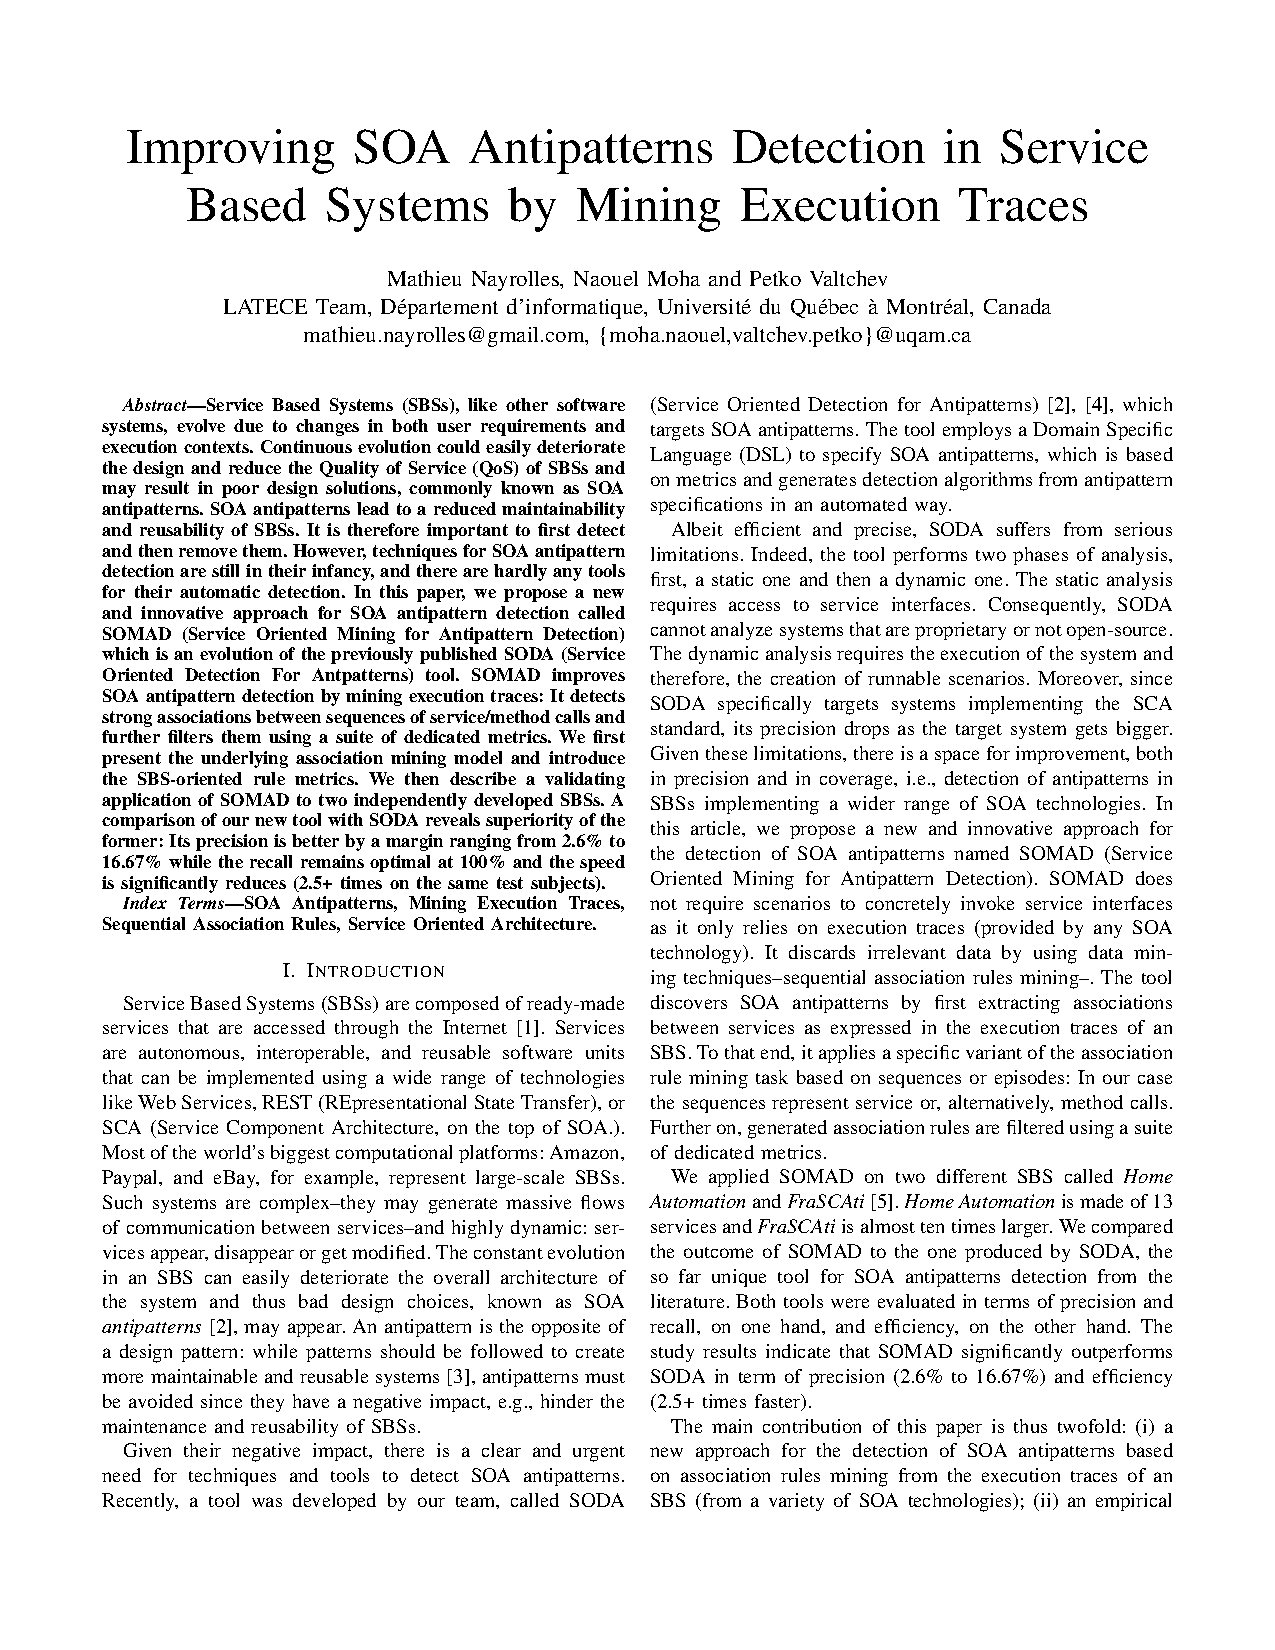
\includepdf[pages=-,pagecommand=\thispagestyle{plain}]{media/WCRE.pdf}

\end{appendices}

\bibliographystyle{apalike-uqam}
\bibliography{my_papers}
\end{document}
